\chapter{Oil Contamination and Cross-species Adulteration}
\label{chapter:oil-contamination-and-cross-species-adulteration}

Continuing the exploration of REIMS data applications, \Cref{chapter:oil-contamination-and-cross-species-adulteration} shifts focus to the critical area of food safety and fraud detection by investigating more nuanced analytical challenges. This chapter details the methodologies developed for detecting oil contamination at various concentration levels and identifying cross-species adulteration in fish samples. It extends the use of the advanced machine learning models from the previous chapter, including Mixture of Experts and Ensemble Transformers, and introduces new strategies such as unsupervised pre-training and a systematic investigation of transfer learning. This investigation is bolstered by detailed ablation studies on both the MoE architecture and the transfer learning process itself. Furthermore, the chapter includes a comparative analysis of ordinal classification techniques to determine the most effective methods for handling graded contamination data. The chapter presents the experimental design, results, computational cost, and a discussion on the models' abilities to discern subtle chemical signatures indicative of contamination or mixing. Similarly to the previous chapter, a strong emphasis is placed on explainability, using LIME to elucidate the specific spectral features that the models associate with different types and levels of contamination, further validating their analytical relevance.

\section{Chapter Overview}

% TODO [x] Bing - Need to include motivations for why doing this research.

Traditional approaches to food safety have struggled to keep pace with the complexities of modern supply chains, where issues like cross-species adulteration and chemical contamination pose significant risks to economic integrity and public health. Adulteration, where high-value products are fraudulently mixed with cheaper species, not only deceives consumers but can also introduce health hazards, an issue brought to the forefront by incidents like the 2013 European Horse Meat Scandal \citep{Premanandh2013} that eroded consumer trust in food supply chains. Similarly, oil contamination from sources like boat engines or factory equipment \citep{Moens2003} can render seafood unsafe for consumption, necessitating effective detection systems to catch contaminants early. While Rapid Evaporative Ionization Mass Spectrometry (REIMS) \citep{Schaefer2009} has been applied to foundational tasks like species identification, its potential for addressing these more nuanced food safety challenges has been largely unexplored. The existing analytical methods are often not equipped to detect the subtle chemical signatures of graded contamination levels or complex mixtures, necessitating the formalization of new analytical tasks and the development of more powerful, data-informed models.

This chapter addresses this gap by formalizing and solving two novel food safety problems for REIMS analysis: oil contamination detection and cross-species adulteration identification. The emerging field of deep learning provides a powerful framework for these new challenges, capable of learning complex feature representations directly from raw data \citep{Goodfellow2016}. However, applying these models presents its own difficulties. The chemical signals for these tasks can be subtle and overlapping, and the models must perform well despite the inherent scarcity of labeled training samples. Furthermore, for any model to be adopted in a food safety context, its decisions must be transparent and verifiable by domain experts in chemistry and fish processing.

This chapter aims to resolve these issues by proposing a novel application of deep learning methods to these newly formalized tasks. The solution is built on a framework of advanced Transformer-based models, which are adept at capturing the complex, non-linear relationships in the REIMS spectra \citep{Vaswani2017}. To learn the sequential patterns of REIMS at multiple scales, we utilize stacked voting ensemble classifiers with multi-scale transformers \citep{Wolpert1992}. To scale to larger models while keeping the cost of inference down, we implement Mixture of Expert Transformers \citep{Jacobs1991,Kaiser2017}. To mitigate small sample sizes and leverage knowledge across different but related tasks, the framework employs transfer learning, allowing a model pre-trained on a source task to be fine-tuned on a target task, proving especially effective for more difficult analyses \citep{Bozinovski1976,Tan2018}. This approach includes implementing unsupervised pretraining to learn robust feature representations from unlabeled data before fine-tuning on a specific task \citep{Devlin2018}, and Transfer Learning (supervised pretraining on other labeled datasets with fine-tuning on another task-specific dataset\citep{Tan2018}). Crucially, this chapter finds that the difficult task of oil contamination detection consistently benefits from knowledge transfer, regardless of the source task. Furthermore, the chapter includes a detailed analysis of ordinal classification techniques, evaluating how different methods handle the graded nature of contamination data and highlighting the trade-offs between classification accuracy and error distance.

This contribution innovates existing work by being the first to apply REIMS-based analysis to oil contamination detection and the first to use it for cross-species adulteration in marine biomass. By successfully adapting and applying a suite of advanced deep learning models to these problems, this chapter establishes a new, high-performance benchmark for food safety analysis. To ensure transparency, the framework employs Local Interpretable Model-agnostic Explanations (LIME) \citep{Ribeiro2016} and Gradient-weighted Class Activation Mapping (Grad-CAM) \citep{Selvaraju2017}, allowing domain experts to understand and validate the molecular features driving model decisions. This work provides a new and powerful capability for REIMS analysis, directly enhancing food safety and fraud prevention in the seafood industry.

\subsection{Contributions}

The main contributions of the chapter are:

\begin{enumerate}
    \item This chapter proposes a novel unsupervised pretraining technique suited toward REIMS mass spectral data. The proposed method is called ``Masked Spectra Modelling" or MSM for short. Experimental results show that unsupervised pretraining increases the balanced accuracy score across four classification tasks. As far as the authors are aware, this is the first application of unsupervised pretraining and Transformers to REIMS-based marine biomass analysis.
    \item This chapter proposes the novel application of transfer learning to a MoE Transformer for REIMS-based marine biomass analysis. The method is called ``A Fish Out of Data", a pun on ``A fish out of water", highlighting the lack of training data available, which motivates the use of transfer learning. Transfer learning is applied to mutually exclusive tasks with mixed results, finding that more difficult tasks benefit from transfer learning. As far as the authors are aware, this is the first application of transfer learning to REIMS-based marine biomass analysis.
    \item This chapter provides a comparative analysis of four approaches to ordinal classification. The analysis demonstrates that methods explicitly designed for ordinal data, such as CORAL and CLM, provide a superior balance between classification accuracy and error distance (MAE), underscoring the importance of selecting a model that aligns with the data's inherent structure.
\end{enumerate}

\section{Transformed-based Pretraining and Transfer Learning}

This chapter introduces the Masked Spectra Modeling pre-training technique and Transfer Learning for transformer models. The core machine learning models and analytical framework used in this chapter are consistent with those detailed in Chapter 4. Specifically, the Transformer architecture (Section 4.2.1), the MoE Transformer (Section 4.2.2), the Ensemble Transformer (Section 4.2.3), and the benchmark methods (Section 4.4) are employed without modification unless otherwise stated. The purpose of this section is to outline the experimental parameters and any task-specific considerations for oil contamination and cross-species adulteration.

For this chapter, there are two ordinal classification datasets, e.g., oil contamination and cross-species adulteration detection. The oil contamination dataset has seven different concentrations of oil, e.g., 50\%, 25\%, 10\%, 5\%, 1\%, 0.1\%, and 0\%. The various concentrations of oil are designed to simulate oil contamination and to detect how fine-grained the REIMS analysis is at picking it up. The cross-species adulteration dataset has three classes, e.g., pure hoki, pure mackerel, and mixed-hoki-mackerel. The mixed samples are designed to simulate cross-species adulteration in seafood products.

To ensure a fair comparison, the model hyperparameters, detailed in \Cref{tab:transformer-parameters-chp-5}, were kept consistent with the previous chapter.
As OPLS-DA \citep{Bylesjoe2006} is the standard technique for biomass analysis in the literature, it continues to serve as the primary benchmark against which our deep learning models are evaluated.

\subsection{Pre-training with Masked Spectra Modelling}

Unsupervised pre-training is utilized to improve Transformer performance, a crucial strategy when dealing with the often-limited availability of labeled mass spectrometry data. This approach allows the model to first learn general underlying patterns and relationships from large-scale, unlabeled datasets. By doing so, the model creates robust, domain-specific feature representations, or embeddings, that can serve as a powerful starting point for subsequent fine-tuning on specific downstream classification tasks, enhancing overall model efficacy.

The primary pre-training technique employed is Masked Spectra Modeling (MSM), which is inspired by the Masked Language Modeling (MLM) concept from BERT. In this approach, instead of masking tokens within a sentence, a portion of the $m/z$ ratios in a given spectrum is masked out. The model is then trained on the objective of predicting these masked values. This is framed as a regression task, where the model is optimized to minimize the mean squared error (MSE) between its predictions and the true $m/z$ values.

To implement MSM for spectral data, a left-to-right progressive masking technique is applied, as illustrated in \Cref{fig:masking-spectra-modelling}. This method generates a multitude of training examples from a single spectrum by creating versions with progressively more of the sequence revealed, which significantly amortizes the limited number of available samples. For instance, a dataset of just 72 samples with 2,080 features each can yield nearly 150,000 unique training instances. By learning to predict these missing values, the model develops a nuanced understanding of the intricate feature relationships within the spectra.

To adapt this pre-trained model for a downstream classification task, the regression head used for MSM is discarded and replaced with a new, task-specific classification head. The core of the model, the pre-trained stack of Transformer encoders, is preserved, and its learned weights provide a strong initialization for the next stage. The entire network---the pre-trained base and the new head---is then trained end-to-end on the labeled dataset. This process only slightly adjusts, or ``fine-tunes,'' the existing weights, adapting the model's general knowledge to the specifics of the new task. Consequently, this foundation leads to improved accuracy, faster convergence, and better generalization when the model is later fine-tuned on labelled datasets.

\begin{figure}[t]
    \centering
    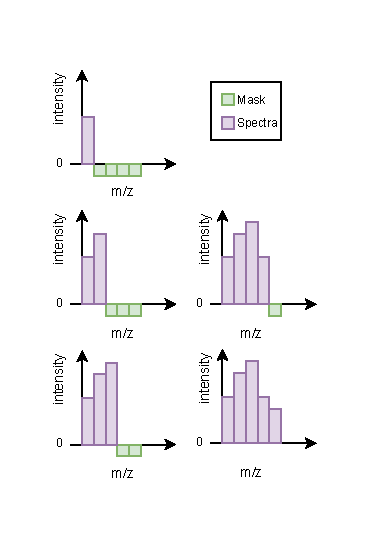
\includegraphics[width=0.4\linewidth]{assets/masked-language-modelling.pdf}
    \caption{Masked Spectra Modelling is a variation of Masked Language Modeling from BERT \cite{Devlin2018}. But unlike BERT, which uses a bidirectional/non-causal approach to predict masked tokens, we use a progressive left-to-right (causal) masking technique, similar to large language models like GPT \citep{Radford2018}. This progressively unmasks spectra, e.g., starting from all spectra masked except one (top left), then unmasking spectra from left to right one by one, until the entire spectra are shown (bottom right). During this unsupervised pre-training task, the model is expected to predict the masked spectra.}    \label{fig:masking-spectra-modelling}
    \end{figure}

\subsection{Transfer Learning Protocol}

Transfer learning \citep{Bozinovski1976,Tan2018} is employed to leverage knowledge from a pre-trained model for new, related tasks, a strategy that can significantly enhance performance and training efficiency. The core principle involves transferring the learned weights and biases from a model that has been pre-trained on a source domain to a new model intended for a target task. As illustrated in the workflow in \Cref{fig:transfer-learning-overview}, an identical model architecture, such as the Mixture of Experts (MoE) Transformer, is first trained on a source dataset. Instead of using random initialization, the weights from this pre-trained model are then used to initialize the new model. This model is subsequently fine-tuned on the target task's training data, a process that typically involves continued training for fewer epochs and with a smaller learning rate to carefully adapt the learned features to the new domain.

To rigorously assess the efficacy of this approach, a controlled experimental procedure is followed. First, a baseline performance is established by training a model with the same architecture directly on the target task's training data, starting from randomly initialized weights. Second, the transfer learning approach is applied: an identical model architecture has its weights initialized from the pre-trained source model and is then fine-tuned on the same target training data. Finally, the performance of both the baseline and the transfer learning models is evaluated, and their balanced classification accuracies are compared. This direct comparison quantifies the impact of the knowledge transfer, demonstrating whether a positive, negative, or neutral transfer effect occurred for the given task.

\begin{figure}
    \centering
    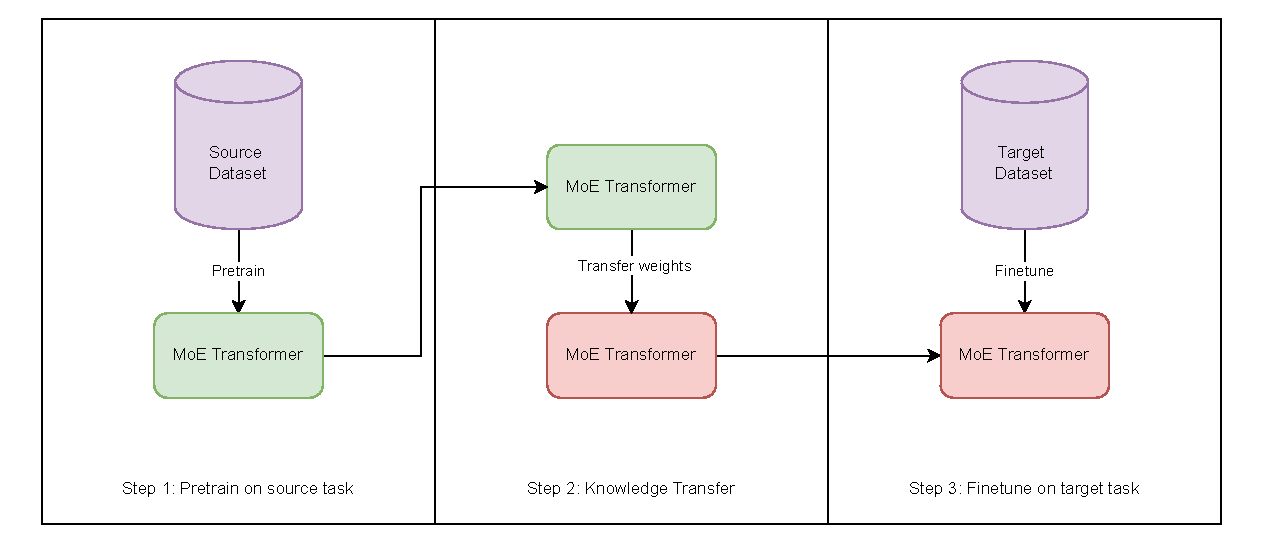
\includegraphics[width=\linewidth]{assets/transfer-learning-overview.pdf}
    \caption{Transfer Learning Overview: The image outlines the transfer learning workflow with MoE Transformers. Step 1 involves pretraining an MoE Transformer on a source dataset. Step 2 shows the knowledge transfer by transferring weights to a new MoE Transformer. Finally, Step 3 depicts finetuning this transformer on a target dataset for the specific target task. }
    \label{fig:transfer-learning-overview}
\end{figure}


\section{Experimental Setup}

Having detailed our methodology, we now describe the experimental framework used to evaluate these approaches. We compare a comprehensive range of machine learning techniques, from traditional methods, advanced deep learning architectures, and evolutionary computation methods, assessing their ability to analyze REIMS data.

\subsection{Benchmark Techniques}

To comprehensively evaluate the performance of the deep learning models proposed in this thesis, we benchmark them against a historical and contemporary suite of analytical methods used for REIMS data. This suite is divided into traditional multivariate (chemometric) techniques and conventional machine learning models.

The analysis of REIMS data has a clear historical progression. The earliest foundational studies relied on simpler methods, such as Principal Component Analysis (PCA) for initial data exploration and dimensionality reduction \citep{Schaefer2009}. This was quickly followed by the use of PCA-Linear Discriminant Analysis (PCA-LDA), which combined dimensionality reduction with a supervised linear classifier, becoming the standard in pioneering medical and food science applications \citep{Balog2010, Balog2013, Balog2016}.

More recently, Orthogonal Partial Least Squares Discriminant Analysis (OPLS-DA) \citep{Bylesjoe2006} became the dominant chemometric method. OPLS-DA improves upon PCA-LDA by explicitly separating the variation in the data into a predictive component (correlated to class labels) and an orthogonal component (uncorrelated). This ability to filter out non-predictive variation makes it highly effective for biomarker discovery and classification in complex datasets. Its strong performance in key food science studies \citep{Verplanken2016, Black2017, Black2019} and its continued use in high-accuracy fish speciation \citep{Shen2020, Shen2022} and traceability \citep{Gkarane2025, Gao2025} establish it as the primary traditional benchmark.

As highlighted in the literature review \citep{Xue2025}, there is a recent trend of applying conventional (non-deep-learning) machine learning models to REIMS data. These models are theoretically better at capturing non-linear relationships than linear methods like OPLS-DA. Therefore, we also include the following as benchmarks:

\begin{itemize}
    \item \textbf{Support Vector Machines (SVM)}
    \item \textbf{Random Forest (RF)}
    \item \textbf{K-Nearest Neighbors (KNN)}
\end{itemize}

The inclusion of these models is critical, as their performance relative to chemometrics is a current topic of discussion. For instance, \citet{De2023} found OPLS-DA to be more robust than RF and SVM for large-scale industrial fish speciation. In contrast, \citet{Lu2024} identified KNN as the superior classifier for geographical authentication of fish. Other studies use them in parallel, for example, applying SVM and RF alongside OPLS-DA for lamb traceability \citep{Gao2025}.

By benchmarking against this entire suite—from foundational PCA and PCA-LDA to the dominant OPLS-DA and the more recent SVM, RF, and KNN—this thesis provides a robust evaluation, comparing the proposed deep learning architectures against the full spectrum of established and contemporary alternatives.

\subsection{Experimental Settings}

To ensure a rigorous and fair comparison, the experimental setup was standardized. Orthogonal Partial Least Squares Discriminant Analysis (OPLS-DA), the standard technique for REIMS analysis in the literature, serves as the primary benchmark against which our models are evaluated.

Model performance was evaluated over 30 independent runs using stratified 5-fold cross-validation to ensure robust results, which is particularly suitable for the limited and imbalanced datasets in this study, because stratification ensures the proportion of classes in each fold is equal to that of the original dataset. To allow for direct comparison with the results from Chapter 4, all deep learning model hyperparameters were kept consistent. The specific parameters for the Transformer architecture are detailed in \Cref{tab:transformer-parameters}.

% TODO [ ] Bing - Why these settings? 

\begin{table}
    \caption{Transformer parameter settings}
    \centering
    \begin{tabular}{ l l }
        \hline
        Learning rate & 1E-5 \\ 
        Epochs & 100 \\
        Dropout & 0.2 \\
        Label smoothing & 0.1 \\
        Early stopping patience & 5 \\
        Optimiser & AdamW \\
        Loss: MSM & MSE \\
        Loss: Cross-species \& Oil & CCE \\
        Input dimensions & 2080 \\ 
        Hidden dimensions & 128 \\
        Output dimensions: MSM & 2080 \\
        Output dimensions: Cross-species & 3 \\
        Output dimensions: Oil & 7 \\
        Number of layers & 4 \\
        Number of heads  & 4 \\
        \hline
    \end{tabular}
    \label{tab:transformer-parameters-chp-5}
\end{table}

We use the parameter settings described in the original paper \citep{Tran2019} for Multiple Class-Independent Feature Construction. A construction ratio of 1 with one tree per class was chosen, in combination with a winner-takes-all strategy to adapt the method for classification. 

\section{Results and Analysis}
\label{sec:results-and-discusssion}

After implementing our classification strategies, we now present and analyze how these various machine learning techniques performed on the REIMS datasets.

\Cref{tab:results_oil} and \Cref{tab:results_cross_species} give the results of the classifiers on the training and test set, 
with the best-performing model on the test set given in \textbf{bold}, and the second-best are given in \textit{italics}. Note that the method \textit{pre-trained} indicates the transformer with progressive left-to-right masked pre-training.

% Table for Oil contamination
\begin{table}[t]
    \centering
    \caption{Classification results for oil contamination detection}
    \label{tab:results_oil}
    \rowcolors{2}{gray!25}{white}
    \begin{tabular}{l|l|l}
        \hline
        Method & Train & Test \\
        \hline
        OPLS-DA & 86.48\% $\pm$ 6.31\% & 26.43\% $\pm$ 6.00\% \\
        KNN & 55.30\% $\pm$ 0.00\% & 25.00\% $\pm$ 0.00\% \\
        DT & 100.00\% $\pm$ 0.00\% & 23.40\% $\pm$ 2.06\% \\
        LR & 100.00\% $\pm$ 0.00\% & 20.89\% $\pm$ 0.00\% \\
        LDA & 70.07\% $\pm$ 0.00\% & 22.86\% $\pm$ 0.00\% \\
        NB & 65.48\% $\pm$ 0.00\% & 25.54\% $\pm$ 0.00\% \\
        RF & 100.00\% $\pm$ 0.00\% & 32.45\% $\pm$ 2.32\% \\
        SVM & 100.00\% $\pm$ 0.00\% & 20.54\% $\pm$ 0.00\% \\
        Ensemble & 100.00\% $\pm$ 0.00\% & 28.13\% $\pm$ 1.00\% \\
        LSTM & 100.00\% $\pm$ 0.00\% & 46.90\% $\pm$ 4.74\% \\
        % 32.28 $\pm$ 4.22
        VAE & 100.00\% $\pm$ 0.00\% & \textit{47.86\% $\pm$ 5.07\%} \\
        % 39.12 $\pm$ 4.75
        KAN & 100.00\% $\pm$ 0.00\% & 44.29\% $\pm$ 3.64\% \\
        CNN & 100.00\% $\pm$ 0.00\% & 41.43\% $\pm$ 8.63\% \\
        Mamba & 100.00\% $\pm$ 0.00\% & 45.95\% $\pm$ 3.42\% \\
        MCIFC & 64.46\% $\pm$ 3.95\% & 38.32\% $\pm$ 8.72\% \\
        Transformer & 100.00\% $\pm$ 0.00\% & 45.19\% $\pm$ 5.73\% \\
        \textit{Pre-trained} & \textit{100.00\% $\pm$ 0.00\%} & \textit{48.57\% $\pm$ 5.07\%} \\
        MoE Transformer & 100.00\% $\pm$ 0.00\% & 45.51\% $\pm$ 5.60\% \\
        \textbf{TL MoE Transformer} & 100.00\% $\pm$ 0.00\% & \textbf{49.10\% $\pm$ 5.85\%} \\
        Ensemble Transformer & 100.00\% $\pm$ 0.00\% & 44.46\% $\pm$ 6.83\% \\ 
        \hline
    \end{tabular}
\end{table}

% Table for Cross-species classification
\begin{table}[t]
    \centering
    \caption{Classification results for cross-species identification.}
    \label{tab:results_cross_species}
    \rowcolors{2}{gray!25}{white}
    \begin{tabular}{l|l|l}
        \hline
        Method & Train & Test \\
        \hline
        OPLS-DA & 100.00\% $\pm$ 0.00\% & 79.96\% $\pm$ 7.50\% \\
        KNN & 81.50\% $\pm$ 0.00\% & 59.38\% $\pm$ 0.00\% \\
        DT & 100.00\% $\pm$ 0.00\% & 63.51\% $\pm$ 1.72\% \\
        LR & 100.00\% $\pm$ 0.00\% & 70.82\% $\pm$ 0.00\% \\
        LDA & 100.00\% $\pm$ 0.00\% & 70.82\% $\pm$ 0.00\% \\
        NB & 72.12\% $\pm$ 0.00\% & 50.35\% $\pm$ 0.00\% \\
        RF & 100.00\% $\pm$ 0.00\% & 63.97\% $\pm$ 2.13\% \\
        SVM & 100.00\% $\pm$ 0.00\% & 69.51\% $\pm$ 0.00\% \\
        Ensemble & 100.00\% $\pm$ 0.00\% & 68.76\% $\pm$ 1.24\% \\
        LSTM & 100.00\% $\pm$ 0.00\% & \textit{91.62\% $\pm$ 5.74\%} \\
        % 64.62 $\pm$ 2.24
        VAE & 93.31\% $\pm$ 7.92\% & 89.84\% $\pm$ 4.98\% \\
        % 79.62 $\pm$ 5.76
        KAN & 100.00\% $\pm$ 0.00\% & 90.92\% $\pm$ 6.62\% \\
        % 75.78 $\pm$ 10.46
        CNN & 100.00\% $\pm$ 0.00\% & 83.03\% $\pm$ 5.48\% \\
        Mamba & 100.00\% $\pm$ 0.00\% & 90.38\% $\pm$ 6.92\% \\
        MCIFC & 82.92\% $\pm$ 4.45\% & 65.85\% $\pm$ 13.66\% \\
        Transformer & 100.00\% $\pm$ 0.00\% & 87.25\% $\pm$ 5.09\% \\
        \textbf{Pre-trained} & 100.00\% $\pm$ 0.00\% & \textbf{91.97\% $\pm$ 4.55\%} \\
        MoE Transformer & 100.00\% $\pm$ 0.00\% & 88.04\% $\pm$ 4.84\%  \\
        TL MoE Transformer & 100.00\% $\pm$ 0.00\% & 83.44\% $\pm$ 6.91\% \\
        \textit{Ensemble Transformer} & 100.00\% $\pm$ 0.00\% & \textit{91.68\% $\pm$ 4.20\%} \\ 
        \hline
    \end{tabular}
\end{table}

We applied multiple machine learning approaches to classify REIMS spectra in marine biomass analysis tasks. The comparative analysis of these models reveals distinct performance patterns, highlighting which techniques excel in specific scenarios while exposing their relative limitations.

\subsection{Overall Performance}

\subsubsection{Oil Contamination}

The low classification accuracy for the oil contamination task, as visualized in the prediction error histogram in \Cref{fig:oil-prediction-error}, is a direct result of the task's inherent difficulty. The thesis describes this as a challenging ordinal multi-class classification problem with seven closely related classes representing different oil concentrations. The histogram shows that while correct predictions (error of 0) are the most common single outcome, there is a wide distribution of errors. This spread is caused by significant 
inter-class similarity, where the chemical signatures of adjacent concentration levels overlap, making the boundaries between them ambiguous. Consequently, the model frequently misclassifies a sample into a neighboring category (errors of -1 or +1), and these frequent, small errors, combined with occasional larger ones, collectively drive down the overall accuracy score.

The confusion matrix in \Cref{fig:oil-confusion-matrix} provides a more granular view of why the accuracy is low, visually confirming the model's struggle with the seven ordinal classes. A high-accuracy model would feature a strong, dark diagonal line, but here the predictions are scattered across multiple cells. This illustrates the model's difficulty in learning the 
fine-grained distinctions between the different oil concentration levels. For example, the model confuses adjacent classes like `2' and `3', and `3' and `4'. Being a 
multi-class problem increases the chance of misclassification, and the ordinal nature means there are subtle, overlapping signals rather than distinct fingerprints for each class. The thesis concludes that these factors make oil contamination detection a fundamentally hard problem, which is clearly reflected in the numerous off-diagonal predictions shown in this matrix.

\begin{figure}
    \centering
    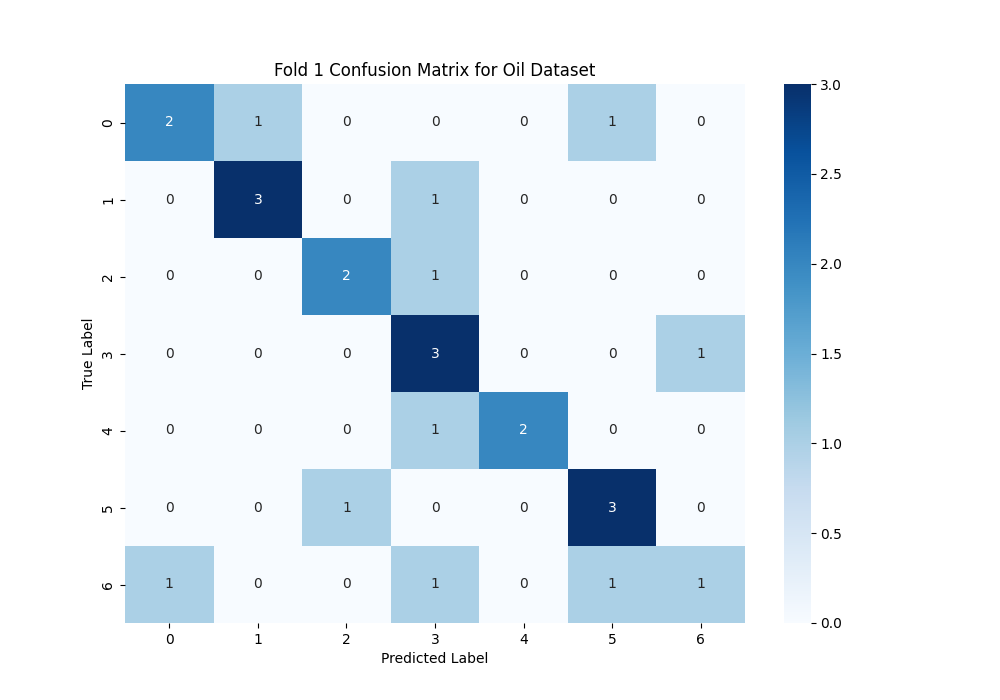
\includegraphics[width=0.7\linewidth]{assets/oil_confusion_matrix_fold_0_1.png}
    \caption{The confusion matrix on the test dataset for one of the folds of cross-validation. The diagonal of the matrix denotes correct class predictions, and all other positions mark incorrect predictions. This is a multi-class classification task with 7 different classes.}
    \label{fig:oil-confusion-matrix}
\end{figure}

\begin{figure}
    \centering
    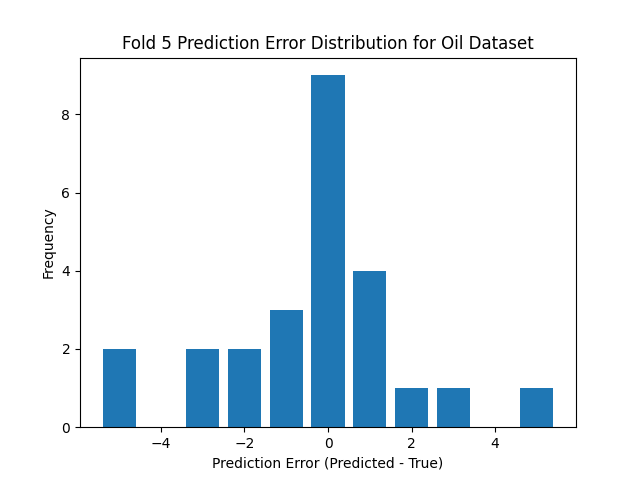
\includegraphics[width=0.7\linewidth]{assets/oil_prediction_error_fold_0_5.png}
    \caption{The prediction error histogram denotes how far off each of the predictions was. Since this is an ordinal classification task, there is overlap between the class labels. Here we see that the plurality of the predictions are the correct class, followed by predictions that are off by one in either direction, then a roughly equal distribution of predictions off by more than 1. The trend is toward correct, or very close to correct, predictions for this ordinal classification task.}
    \label{fig:oil-prediction-error}
\end{figure}

Here we analyze the results listed in \Cref{tab:results_oil}.
While the pre-trained transformer achieved near-perfect accuracy on the simpler species identification task in Chapter 4 (99.62\%), its performance on oil contamination detection (48.57\%) underscores the significant increase in task difficulty.

The MoE model with Transfer Learning achieves the best performance (49.10\%) on the oil contamination dataset, followed in close second by the Pre-trained Transformer (48.57\%).
These models likely excel at this task because oil contamination introduces subtle and nuanced changes in the ionization patterns that require models capable of detecting minor anomalies or deviations in the data. 
By leveraging the generalized representation gained from pre-training and transfer learning, these transformers have learned efficient representations to then be further fine-tuned for the downstream tasks like oil contamination detection. 

Traditional machine learning models struggle with this task, with accuracies ranging from 20.89\% for Logistic Regression to 32.45\% for Random Forest. This poor performance indicates that the signal variations introduced by oil contamination are not easily captured using simple, linear decision boundaries or tree-based splits. The complexity of the task requires more sophisticated feature extraction, something deep learning models like pre-trained Transformers are better equipped to handle.

The pre-trained transformer model (48.57\%) outperforms the OPLS-DA method (26.43\%) by a significant margin for oil contamination multi-class classification. Notably, deep learning methods have bested the traditional approach in the field of REIMS analysis. 

\subsubsection{Cross-species Contamination}

Here we analyze the results listed in \Cref{tab:results_cross_species}.
The pre-trained transformer achieves the highest test accuracy (91.97\%) on the cross-species contamination dataset. The self-attention mechanism in transformers allows each data point (or peak) in the mass spectrum to attend to all other points. This global context awareness is particularly useful in mass spectrometry, where relationships between peaks across the entire spectrum can be important for identification and quantification.
The Ensemble Transformer is the second-best performing model (91.68\%). Mass spectrometry data is inherently sequential, with peaks occurring at different mass-to-charge ratios (m/z). Analyzing these peaks at 3 different resolutions, from low to high, with the stacked voting ensemble classifier of multi-scale transformers, captures the patterns from fine-grain to coarse inherent to the data.

The lower accuracy of this task compared to fish species classification alone \citep{Wood2022} suggests that mixed-species samples introduce additional complexity, making it harder to classify. Cross-species contamination likely involves overlapping patterns from multiple species, which traditional machine learning models find difficult to distinguish, requiring advanced models that can disentangle complex, multi-source signals.

The pre-trained transformer (91.97\%) outperforms the OPLS-DA method (79.96\%) for the task of cross-species contamination. For this second task, deep learning methods exceed the traditional approach of REIMS analysis used in the literature.

\subsubsection{Summary:}

Our experiments reveal three significant findings about machine learning approaches for REIMS data analysis. First, deep learning methods consistently outperform the traditional OPLS-DA method \citep{Verplanken2016,Black2017,Black2019}, with the pre-trained transformer achieving 91.97\% test accuracy in cross-species adulteration detection and the MoE with Transfer Learning reaching 49.10\% test accuracy in oil contamination detection. This represents a substantial improvement over OPLS-DA's 79.96\% and 26.43\%, respectively, suggesting that deep learning should be considered the new standard for REIMS analysis.
Second, different architectures show task-specific strengths. The transformer architecture excels at both cross-species and oil contamination detection, likely due to its ability to capture long-range dependencies in mass spectra.
Third, our results highlight areas requiring further development. While cross-species adulteration detection achieves high accuracy, oil contamination detection remains challenging. This performance gap suggests that detecting subtle chemical changes from oil contamination requires more sophisticated approaches than identifying distinct species-specific molecular signatures.

\subsection{Visualization} 

While our deep learning models achieve high accuracy, their practical adoption in fish processing facilities requires interpretability. Domain experts in chemistry and fish processing need to understand and validate model decisions based on known molecular markers. To achieve this transparency, we employ Local Interpretable Model-agnostic Explanations (LIME) \citep{Ribeiro2016}.
LIME reveals how our models use specific mass spectrometry features (mass-to-charge ratios) to make classifications. For each prediction, LIME creates multiple variations of the input by perturbing feature values and observes how these changes affect the model's output. This sampling process helps construct a simpler, interpretable model that approximates our complex model's behaviour in the local region around the prediction of interest.
We visualize these LIME explanations as bar charts showing the five most influential mass-to-charge ratios for each classification:

\begin{itemize}
    \item Green bars indicate features whose presence supports the predicted class.
    \item Red bars show features whose presence contradicts the predicted class.
    \item Bar length represents the strength of each feature's influence.
    \item The y-axis specifies the mass-to-charge ratio (m/z) and intensity threshold values.
\end{itemize}

This approach lets chemists verify if the model bases its decisions on chemically meaningful markers. For example, when detecting oil contamination, they can confirm if the model identifies mass-to-charge ratios associated with known oil compounds.

\subsubsection{Oil Contamination}
\label{sec:mamba-on-oil-contamination}

The pre-trained transformer model achieves one of the best classification accuracies ($48.57\%$) for the difficult oil contamination task. The following LIME explanations illustrate the distinct shifts in the molecular fingerprint as oil concentration changes, offering chemically relevant insights across the seven ordinal levels.

\Cref{fig:line-pt-transformer-50} reveals the key feature driving the $50\%$ contamination prediction. The strongest indicator (green bar) is the molecular ion $m/z~299.2513$ when its normalized intensity is greater than $0.36$. This high abundance strongly correlates with maximum oil contamination, suggesting this ion is directly associated with the oil profile.

\begin{figure}
    \centering
    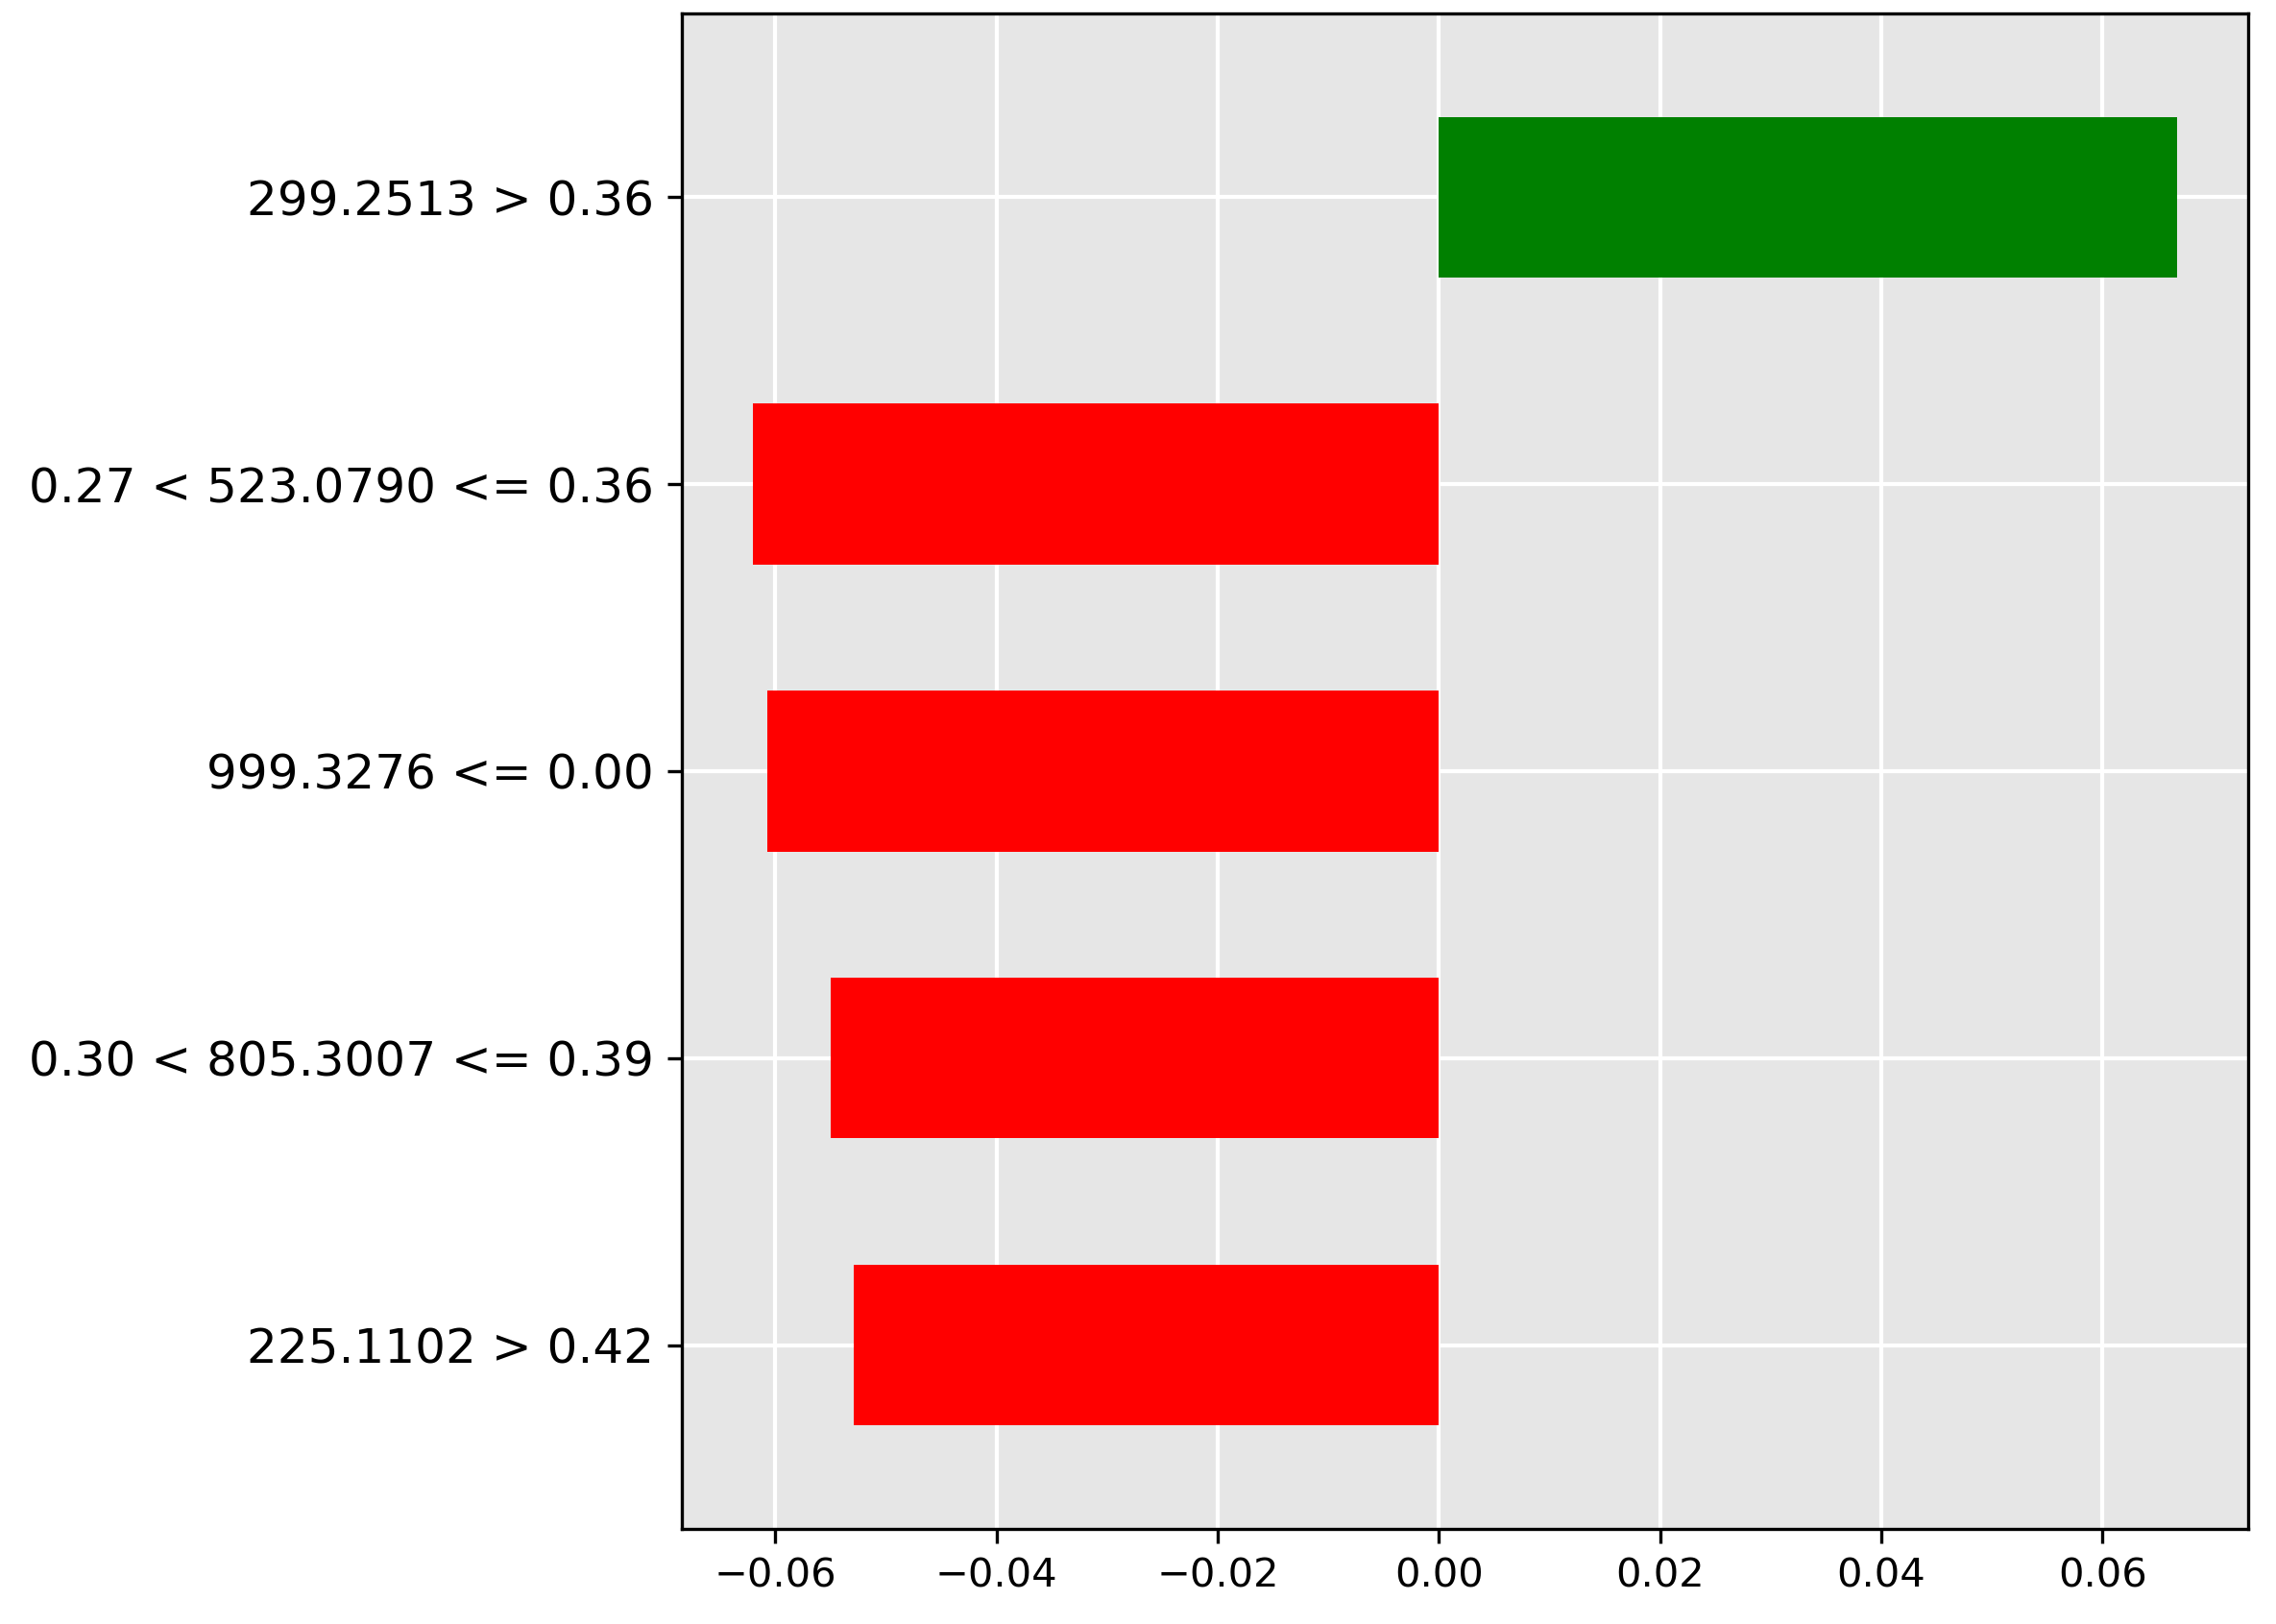
\includegraphics[width=0.7\linewidth]{assets/lime_transformer_oil_50.png}
    \caption{LIME explanation for \textbf{pre-trained transformer} for classification of oil contamination in \textbf{50\%} concentration.}
    \label{fig:line-pt-transformer-50}
\end{figure}

The model’s explanation for $25\%$ contamination (\Cref{fig:line-pt-transformer-25}) shows the most important feature (green bar) is the molecular ion $m/z~592.1977$ when its intensity is $\le 0.28$. This suggests that a low abundance of this ion is characteristic of moderate oil contamination, implying it might be a fish-native metabolite whose concentration is diluted or suppressed by the oil.

\begin{figure}
    \centering
    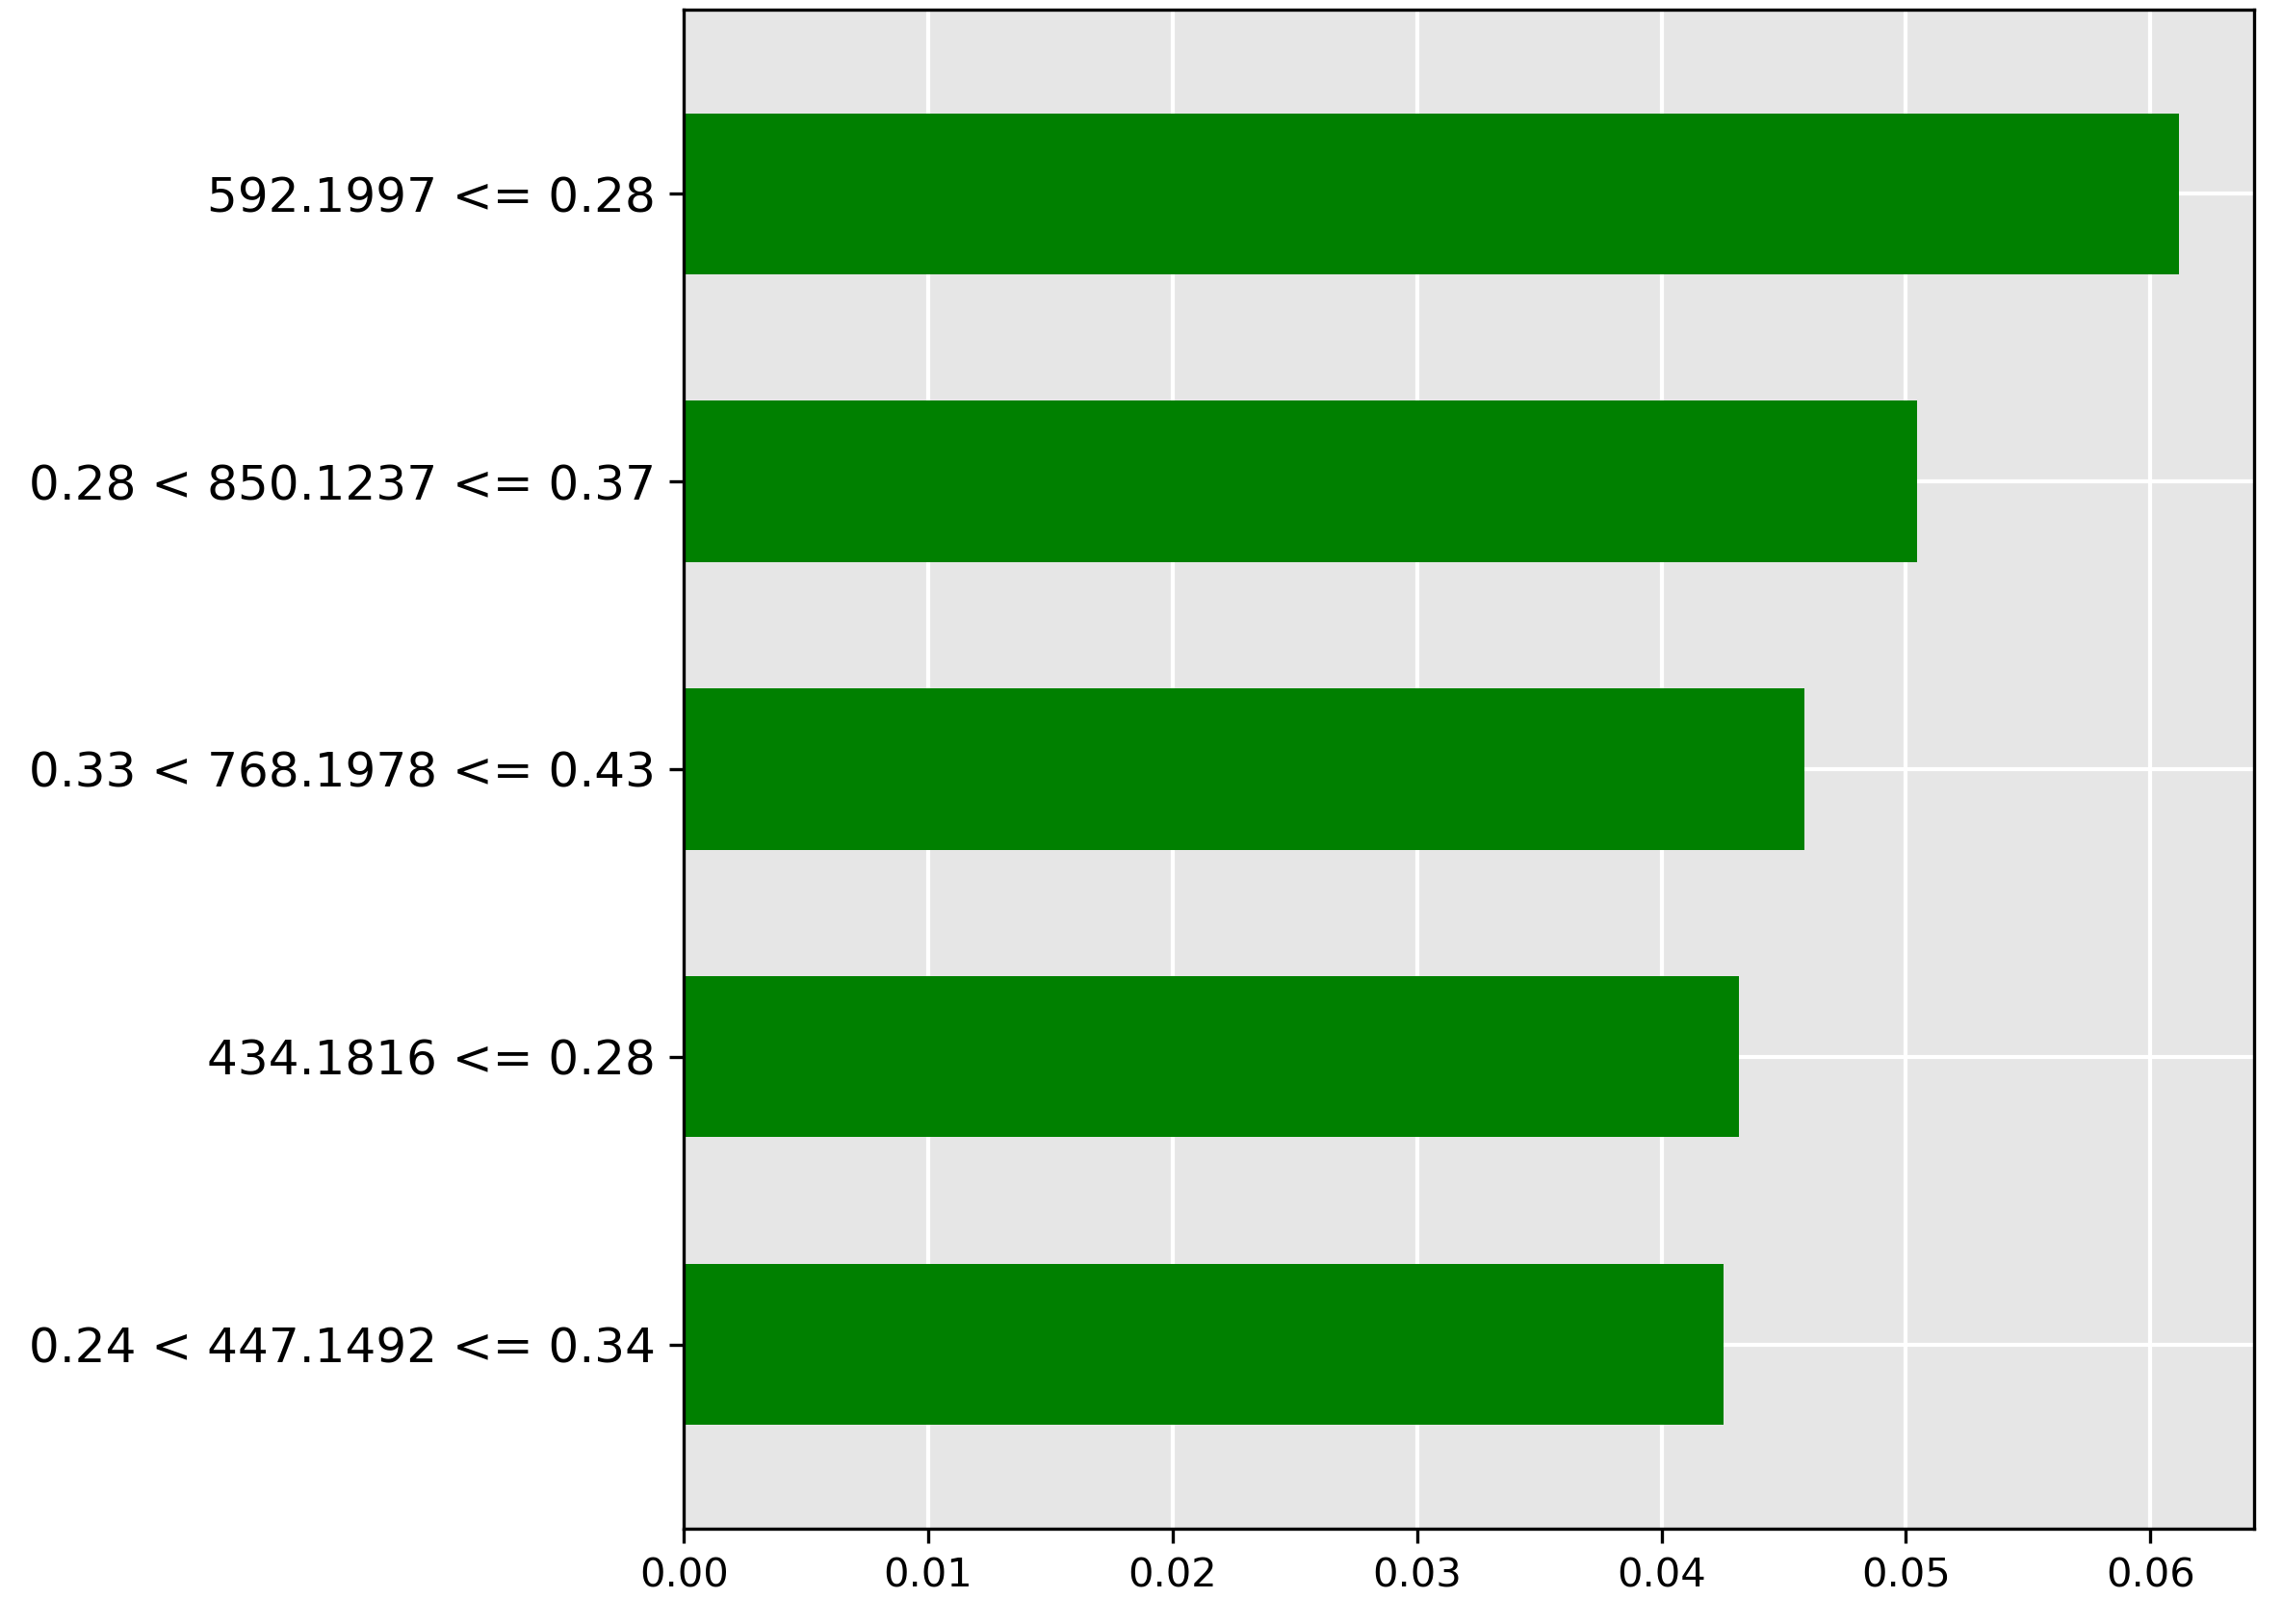
\includegraphics[width=0.7\linewidth]{assets/lime_transformer_oil_25.png}
    \caption{LIME explanation for \textbf{pre-trained transformer} for classification of oil contamination in \textbf{25\%} concentration.}
    \label{fig:line-pt-transformer-25}
\end{figure}

Moving to $10\%$ contamination, \Cref{fig:line-pt-transformer-10} shows the strongest predictive feature (red bar) is the molecular ion $m/z~606.1037$ when its intensity exceeds $0.45$. Since this feature \textbf{negatively} correlates with $10\%$ contamination, its high abundance suggests the sample is either heavily contaminated or completely pure, but \textbf{not} at the $10\%$ threshold.

\begin{figure}
    \centering
    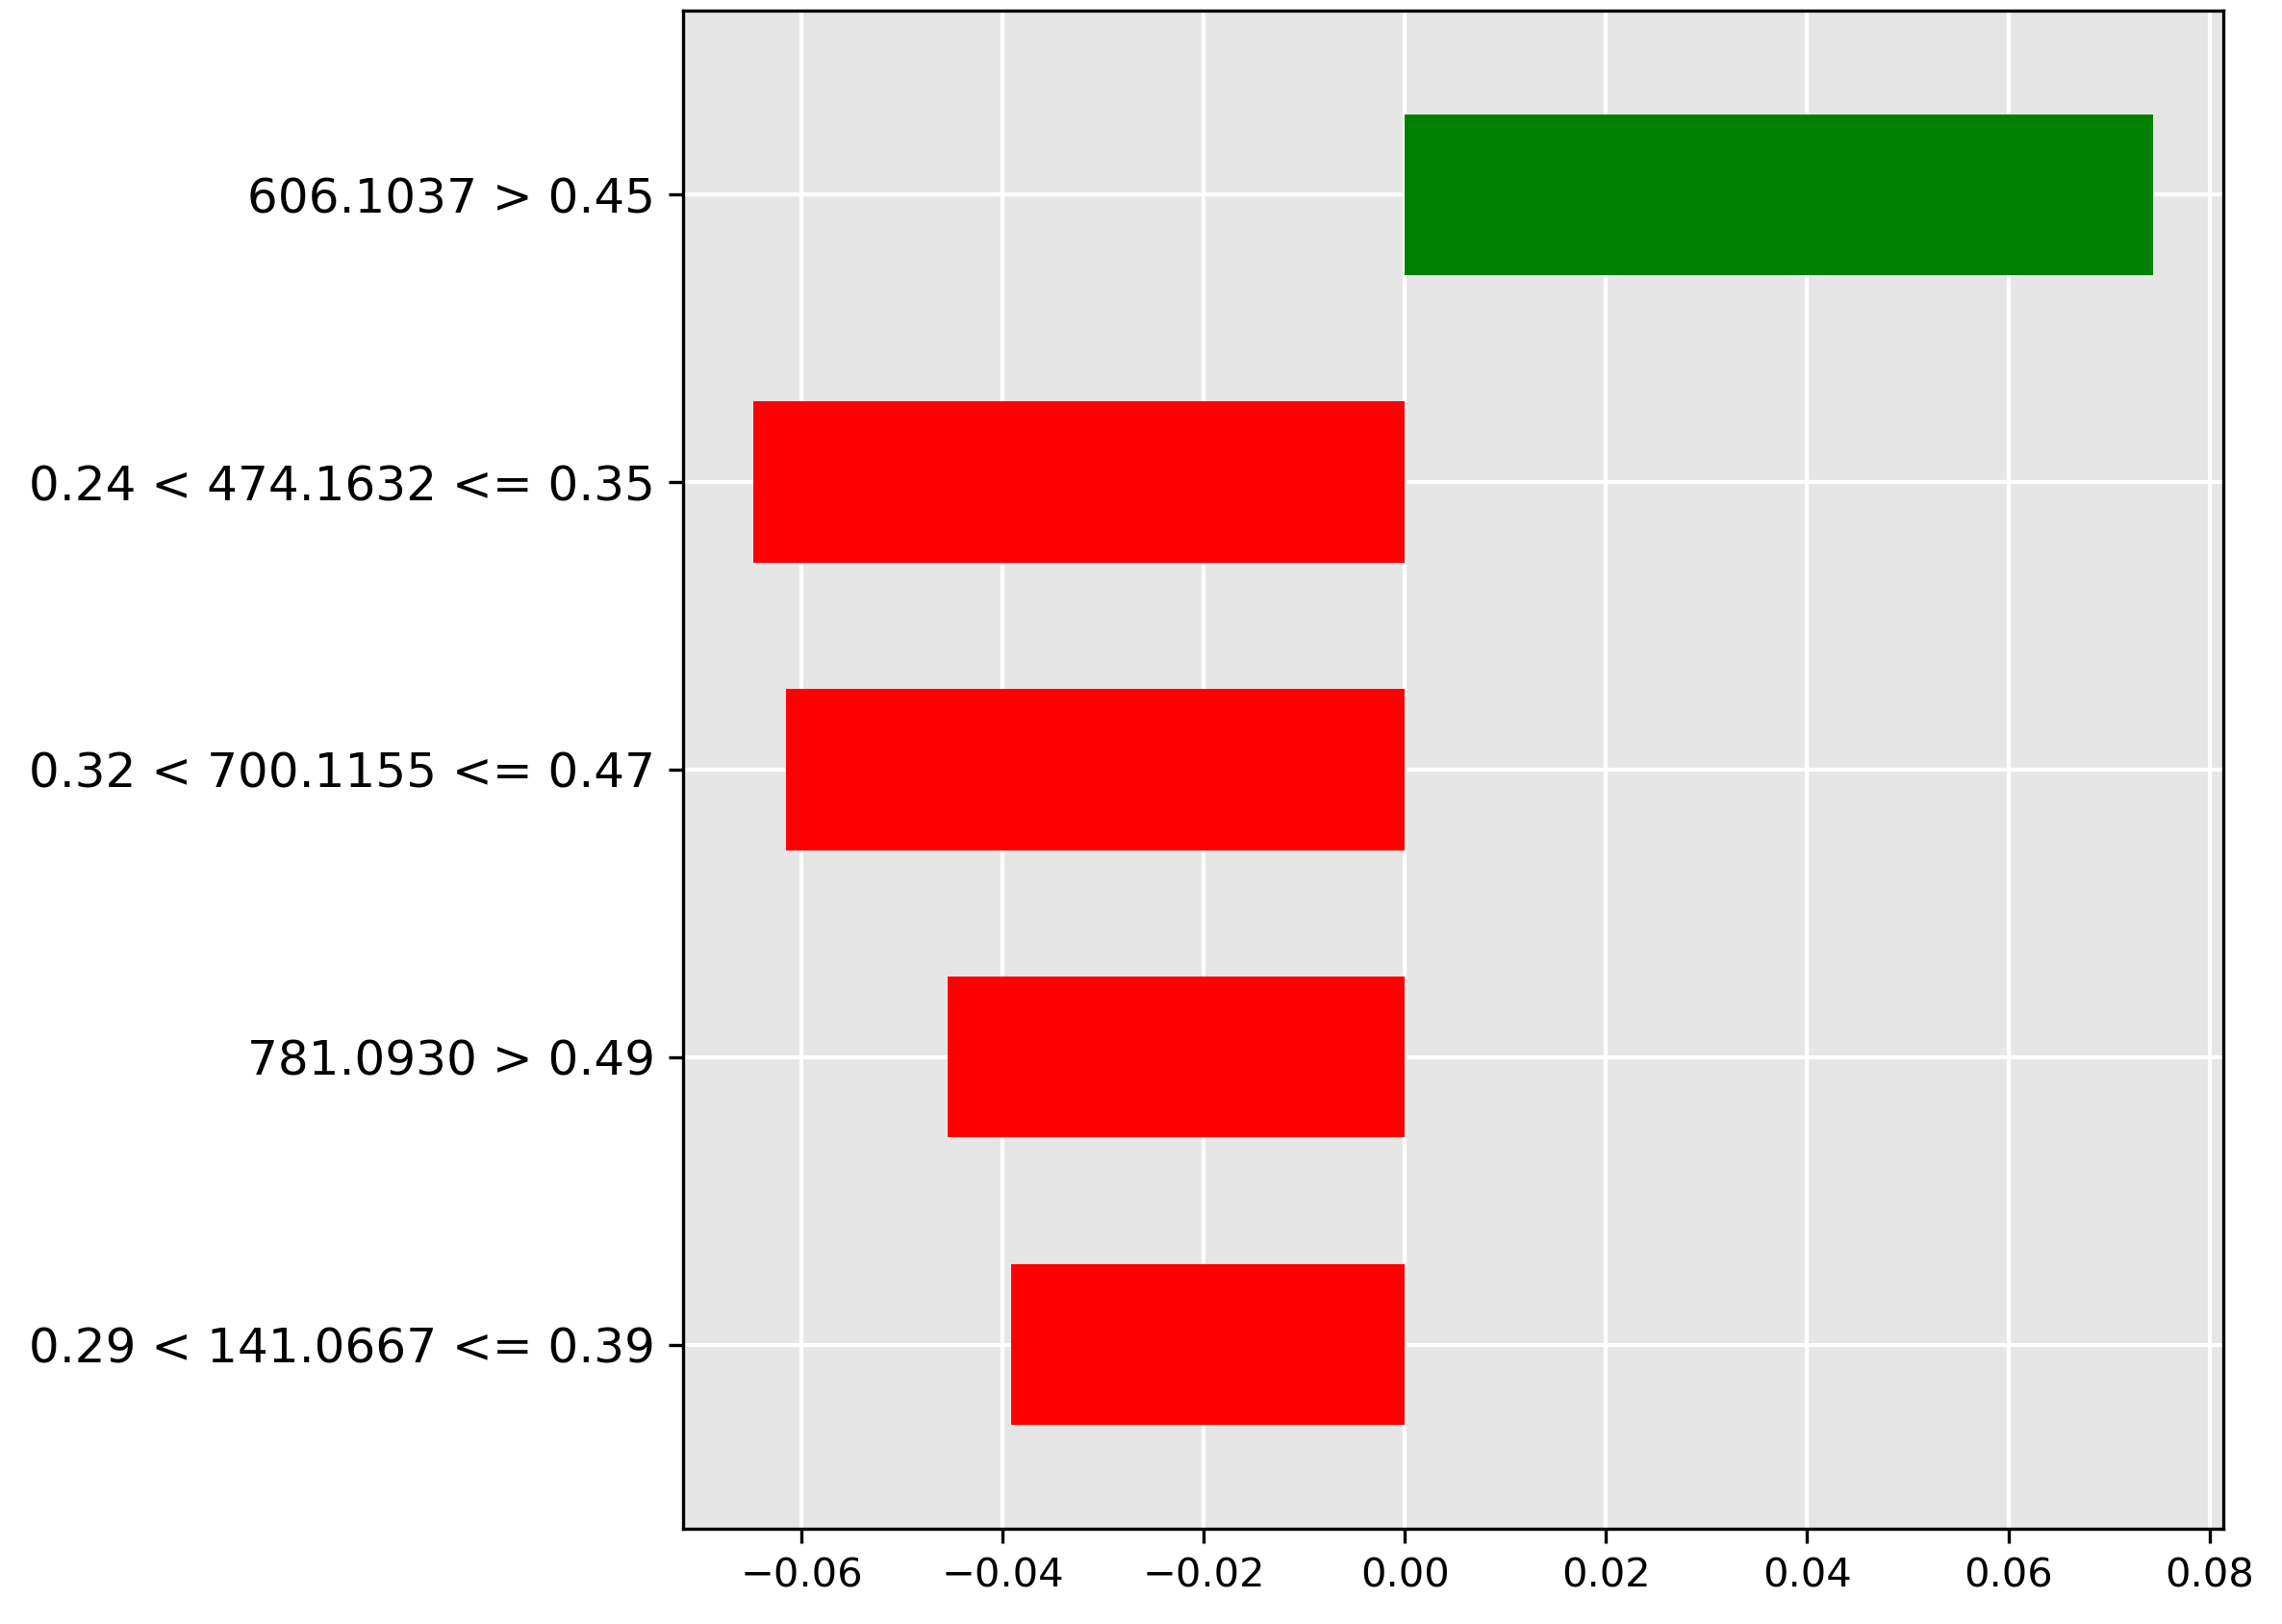
\includegraphics[width=0.7\linewidth]{assets/lime_transformer_oil_10.png}
    \caption{LIME explanation for \textbf{pre-trained transformer} for classification of oil contamination in \textbf{10\%} concentration.}
    \label{fig:line-pt-transformer-10}
\end{figure}

For $5\%$ contamination (\Cref{fig:line-pt-transformer-5}), the model relies on the molecular ion $m/z~619.1768$ (strongest red bar) when its normalized intensity falls in the range $0.27 < y \le 0.40$. This indicates that average amounts of this ion are actively used to rule out low oil contamination.

\begin{figure}
    \centering
    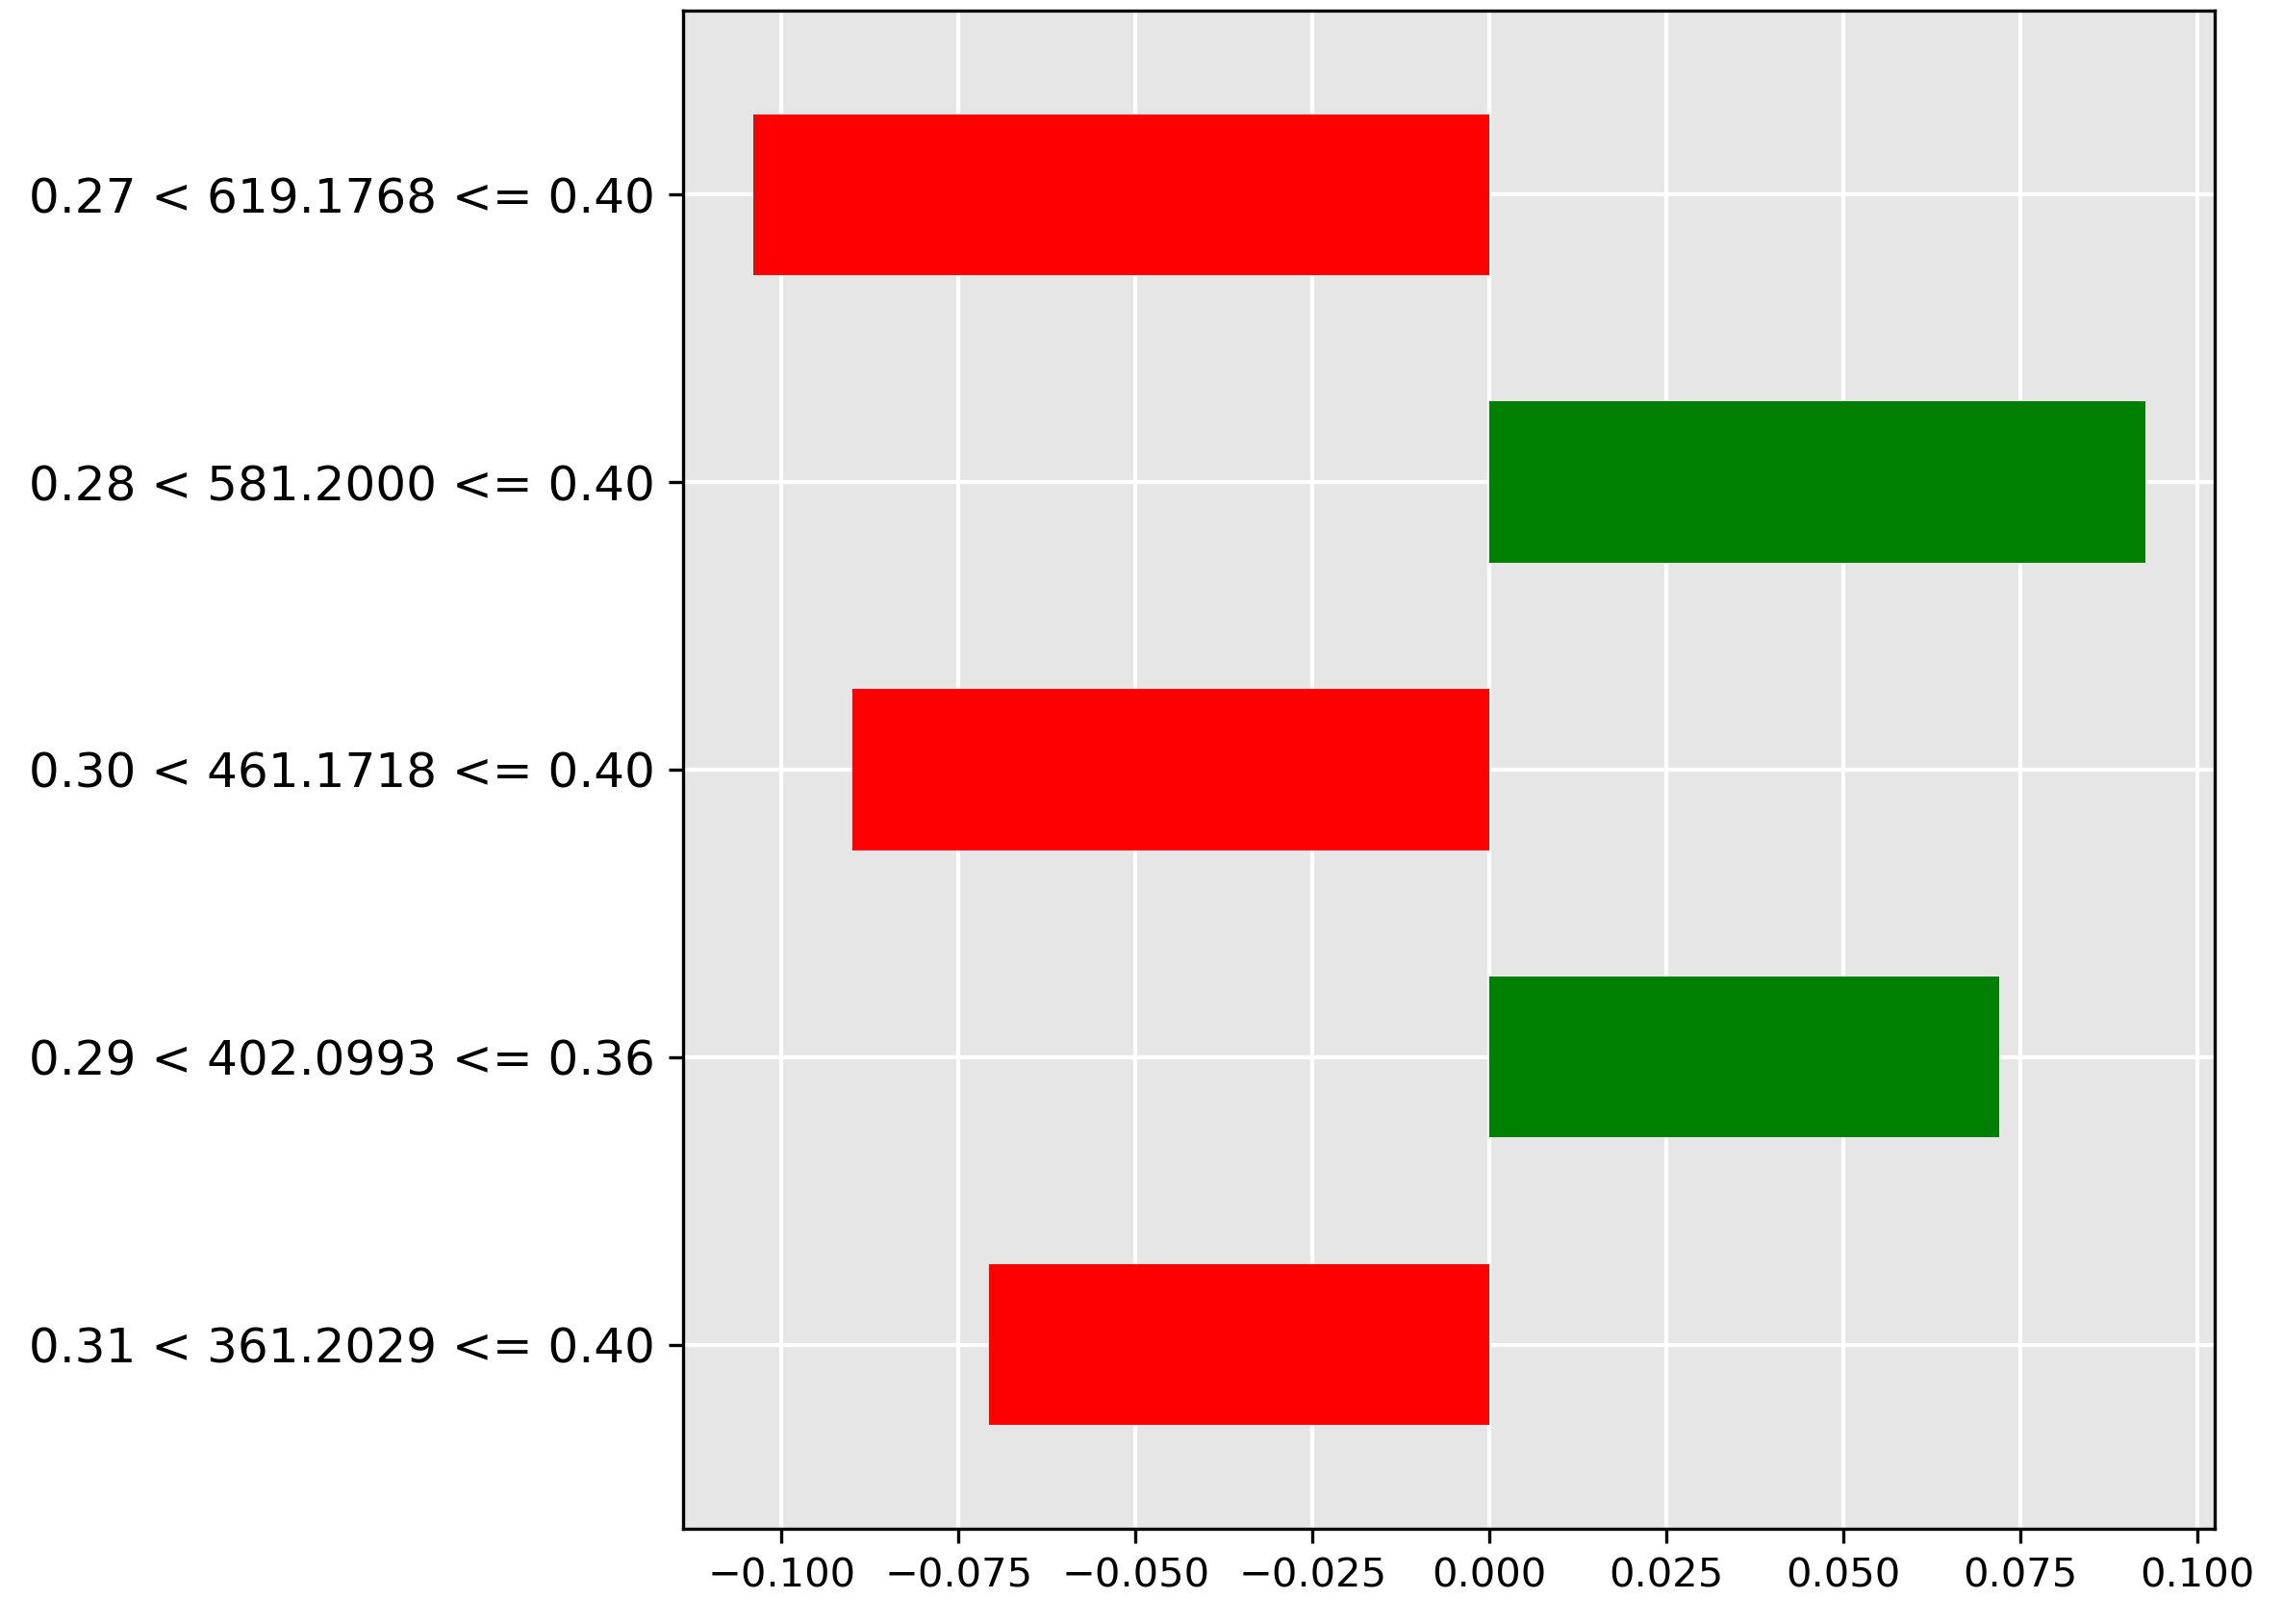
\includegraphics[width=0.7\linewidth]{assets/lime_transformer_oil_5.png}
    \caption{LIME explanation for \textbf{pre-trained transformer} for classification of oil contamination in \textbf{5\%} concentration.}
    \label{fig:line-pt-transformer-5}
\end{figure}

At the $1\%$ level (\Cref{fig:line-pt-transformer-1}), the most important feature (red bar) is $m/z~545.1095$ when its intensity is between $0.39 < y \le 0.50$. This suggests that high-average amounts of the corresponding molecular ion are characteristic of a \textbf{non-trace} oil contamination scenario.

\begin{figure}
    \centering
    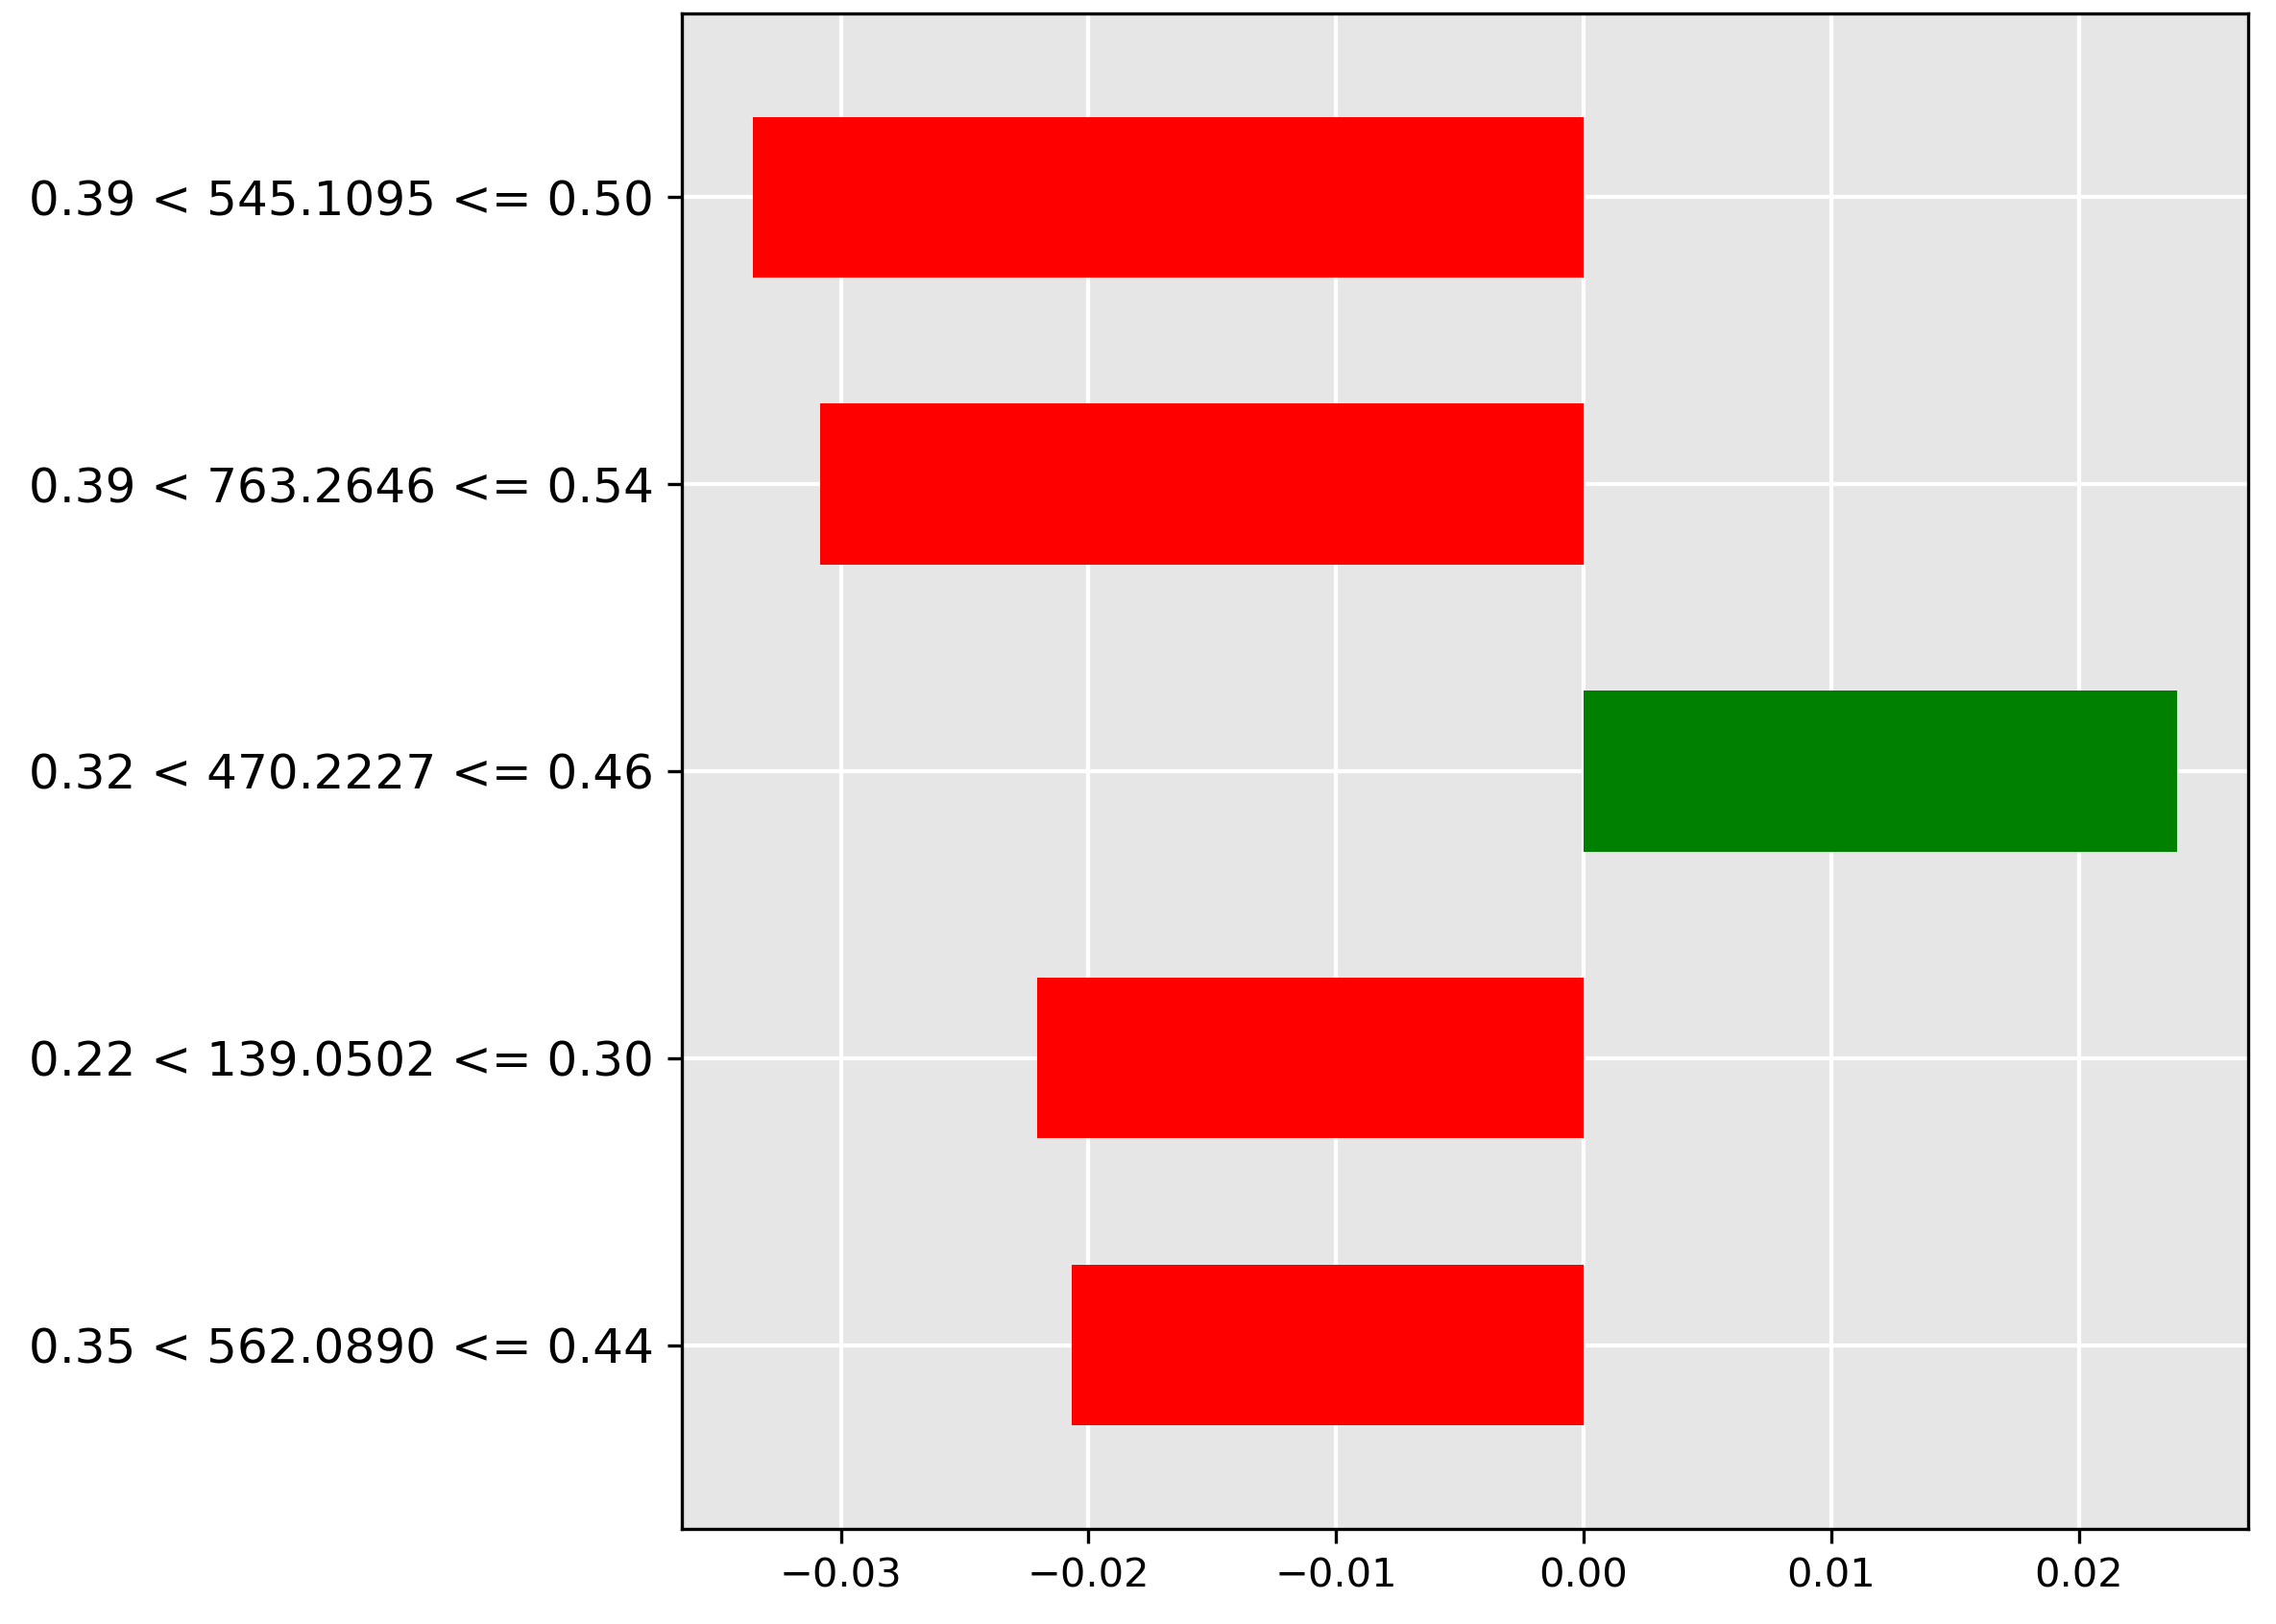
\includegraphics[width=0.7\linewidth]{assets/lime_transformer_oil_1.png}
    \caption{LIME explanation for \textbf{pre-trained transformer} for classification of oil contamination in \textbf{1\%} concentration.}
    \label{fig:line-pt-transformer-1}
\end{figure}

Predicting minuscule $0.1\%$ trace contamination (\Cref{fig:line-pt-transformer-0.1}) is driven away (red bar) by the presence of $m/z~598.2055$ when its normalized intensity is between $0.38 < y \le 0.46$. Since this ion's presence rules out the $0.1\%$ classification, and is negatively correlated with the $0\%$ baseline, the model has likely isolated a molecular ion associated with the oil contaminant itself.

\begin{figure}
    \centering
    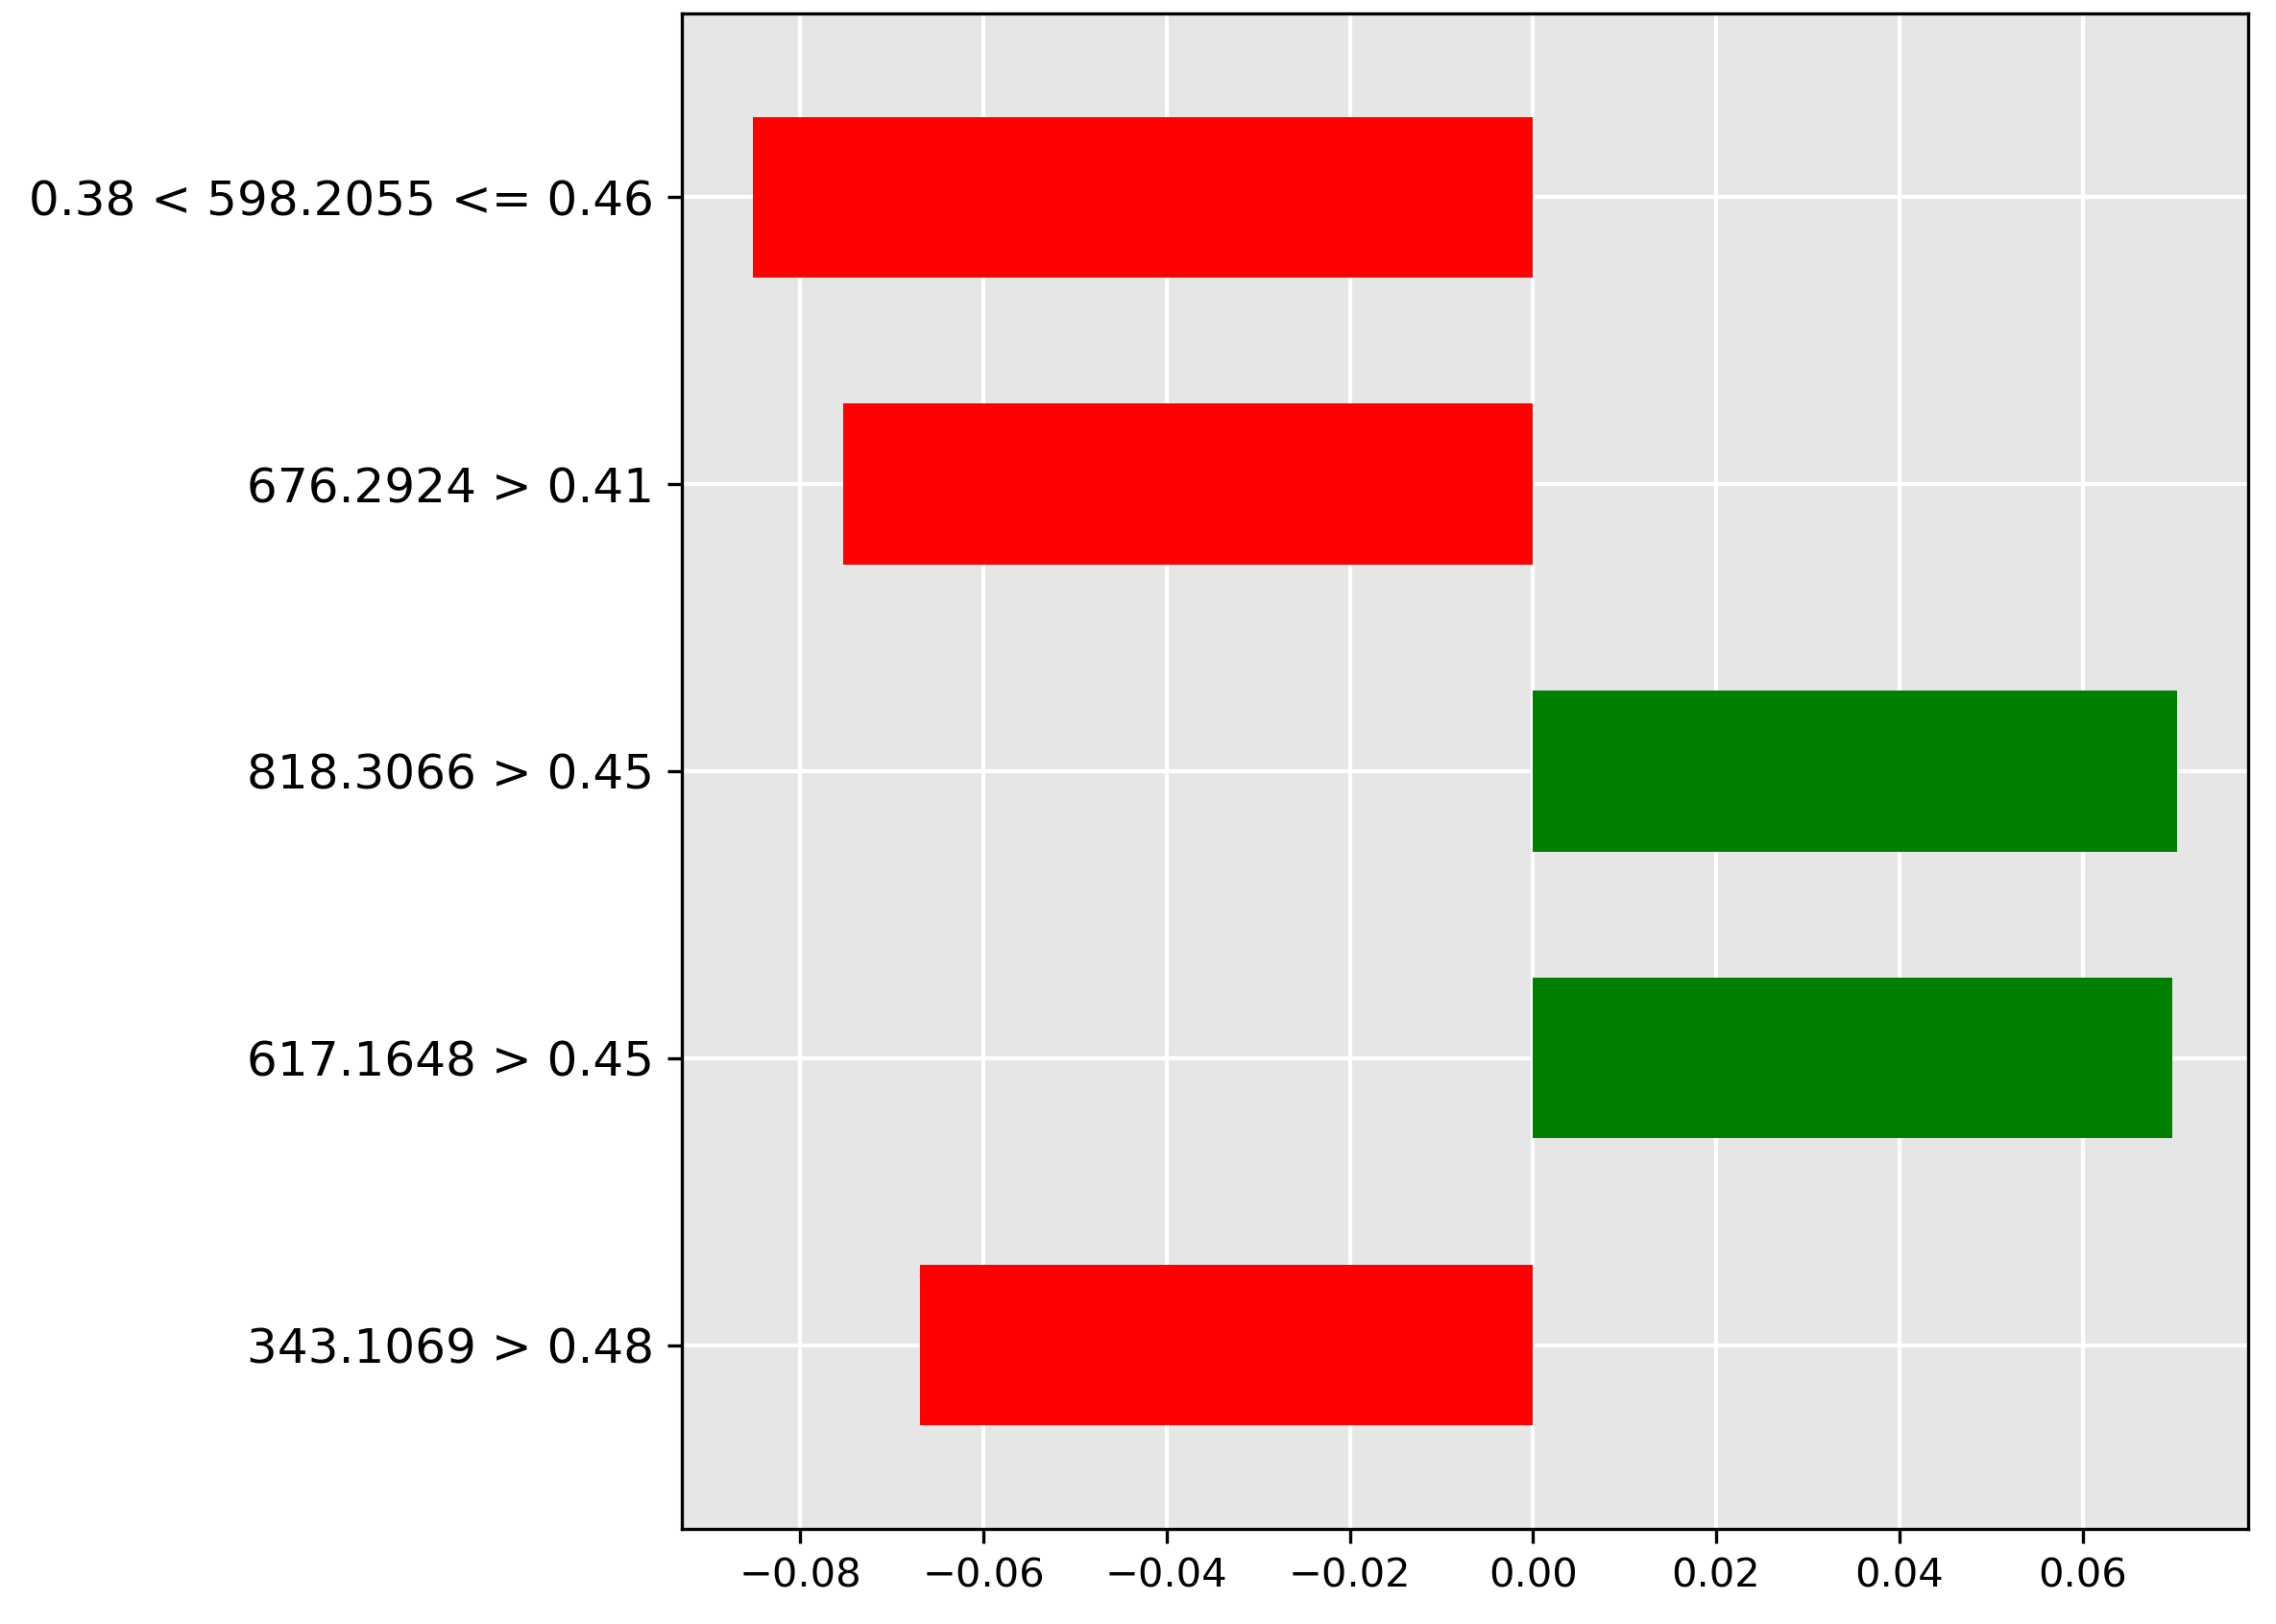
\includegraphics[width=0.7\linewidth]{assets/lime_transformer_oil_0.1.png}
    \caption{LIME explanation for \textbf{pre-trained transformer} for classification of oil contamination in \textbf{0.1\%} concentration.}
    \label{fig:line-pt-transformer-0.1}
\end{figure}

Finally, for the $0\%$ (pure fish) baseline (\Cref{fig:line-pt-transformer-0}), the model key prediction is the high abundance ($> 0.38$) of the molecular ion $m/z~111.0971$ (largest green bar). This ion is chemically hypothesized to be a key native metabolite found consistently in both Hoki and Mackerel.

\begin{figure}
    \centering
    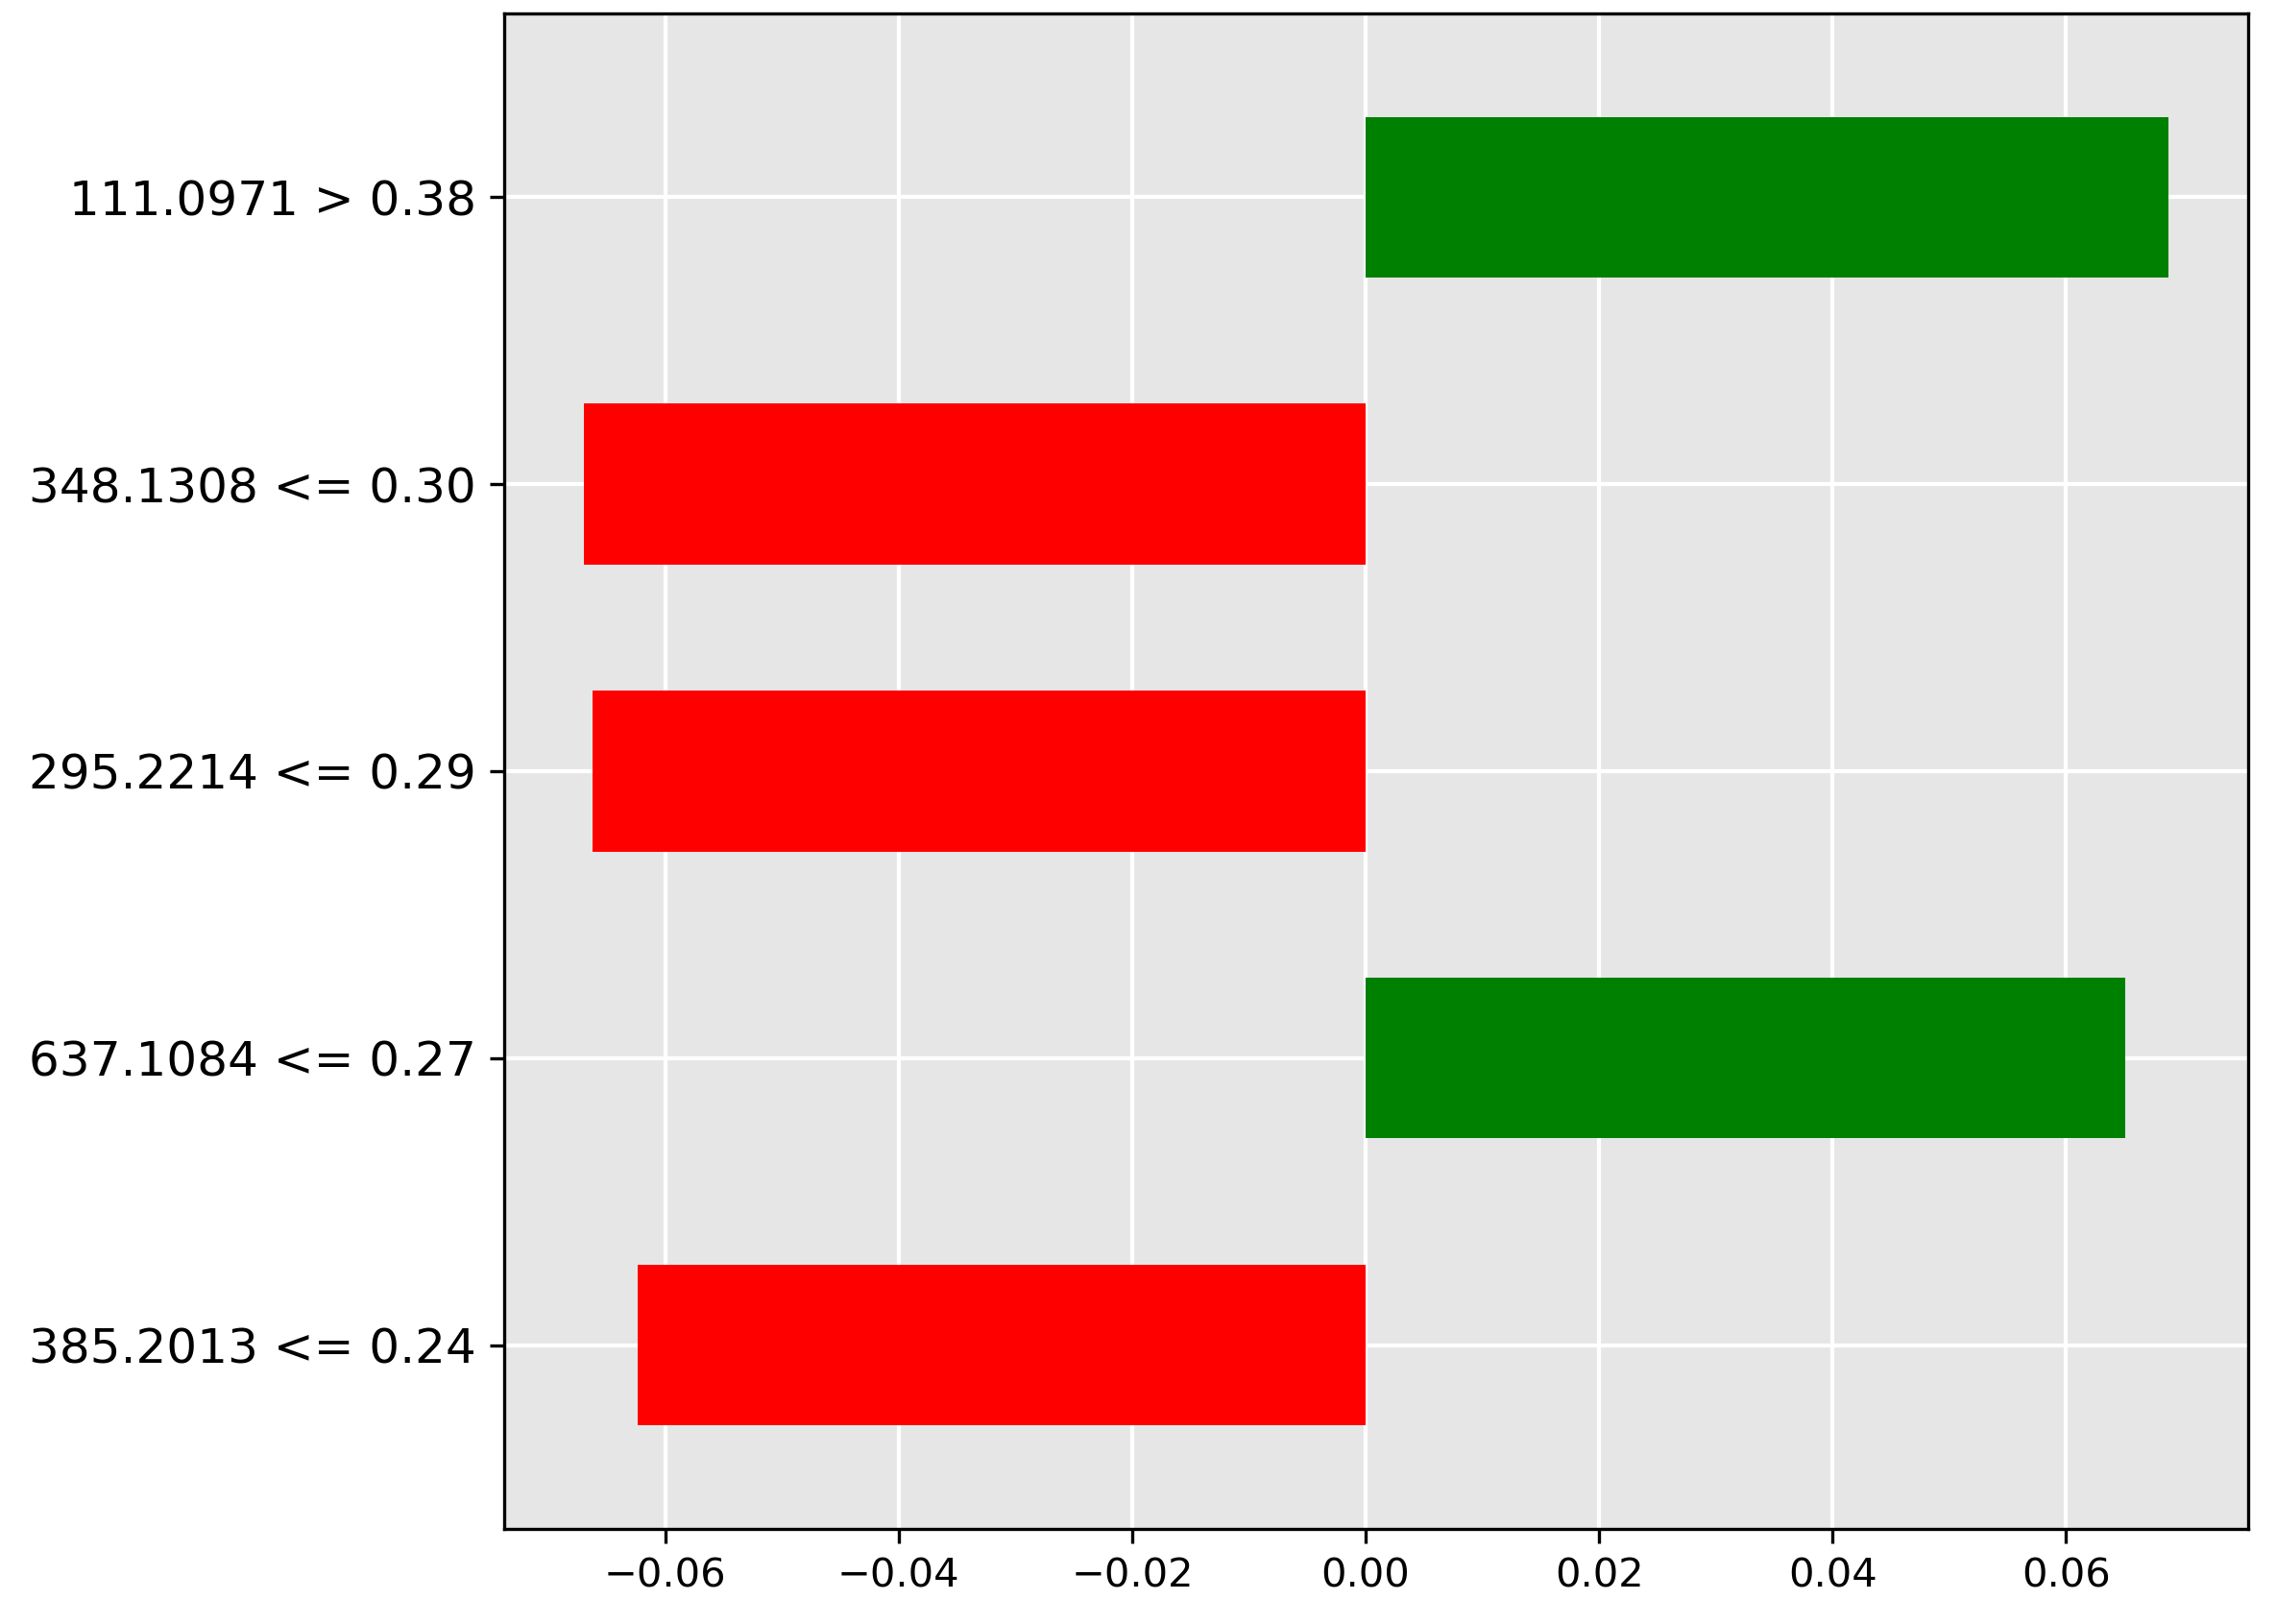
\includegraphics[width=0.7\linewidth]{assets/lime_transformer_oil_0.png}
    \caption{LIME explanation for \textbf{pre-trained transformer} for classification of oil contamination in \textbf{0\%} concentration.}
    \label{fig:line-pt-transformer-0}
\end{figure}

\subsubsection{Cross-Species Contamination}
\label{sec:logistic-regression-on-cross-species-contamination}

The pre-trained transformer performs exceptionally well, achieving the best accuracy ($91.97\%$) on the cross-species contamination task. The LIME results below illuminate the specific spectral features the model uses to distinguish pure species from the mixed adulterated product.

\Cref{fig:lime-transformer-cross-species-hoki-mackerel} shows the predictive features for the difficult \textbf{Hoki-Mackerel mix} class. The strongest negative indicator (red bar) is the low abundance ($\le 0.03$) of the molecular ion $m/z~251.1667$. The model uses the low intensity of this ion to strongly rule out the presence of the mix, suggesting this ion is characteristic of one of the \textbf{pure} species.

\begin{figure}
    \centering
    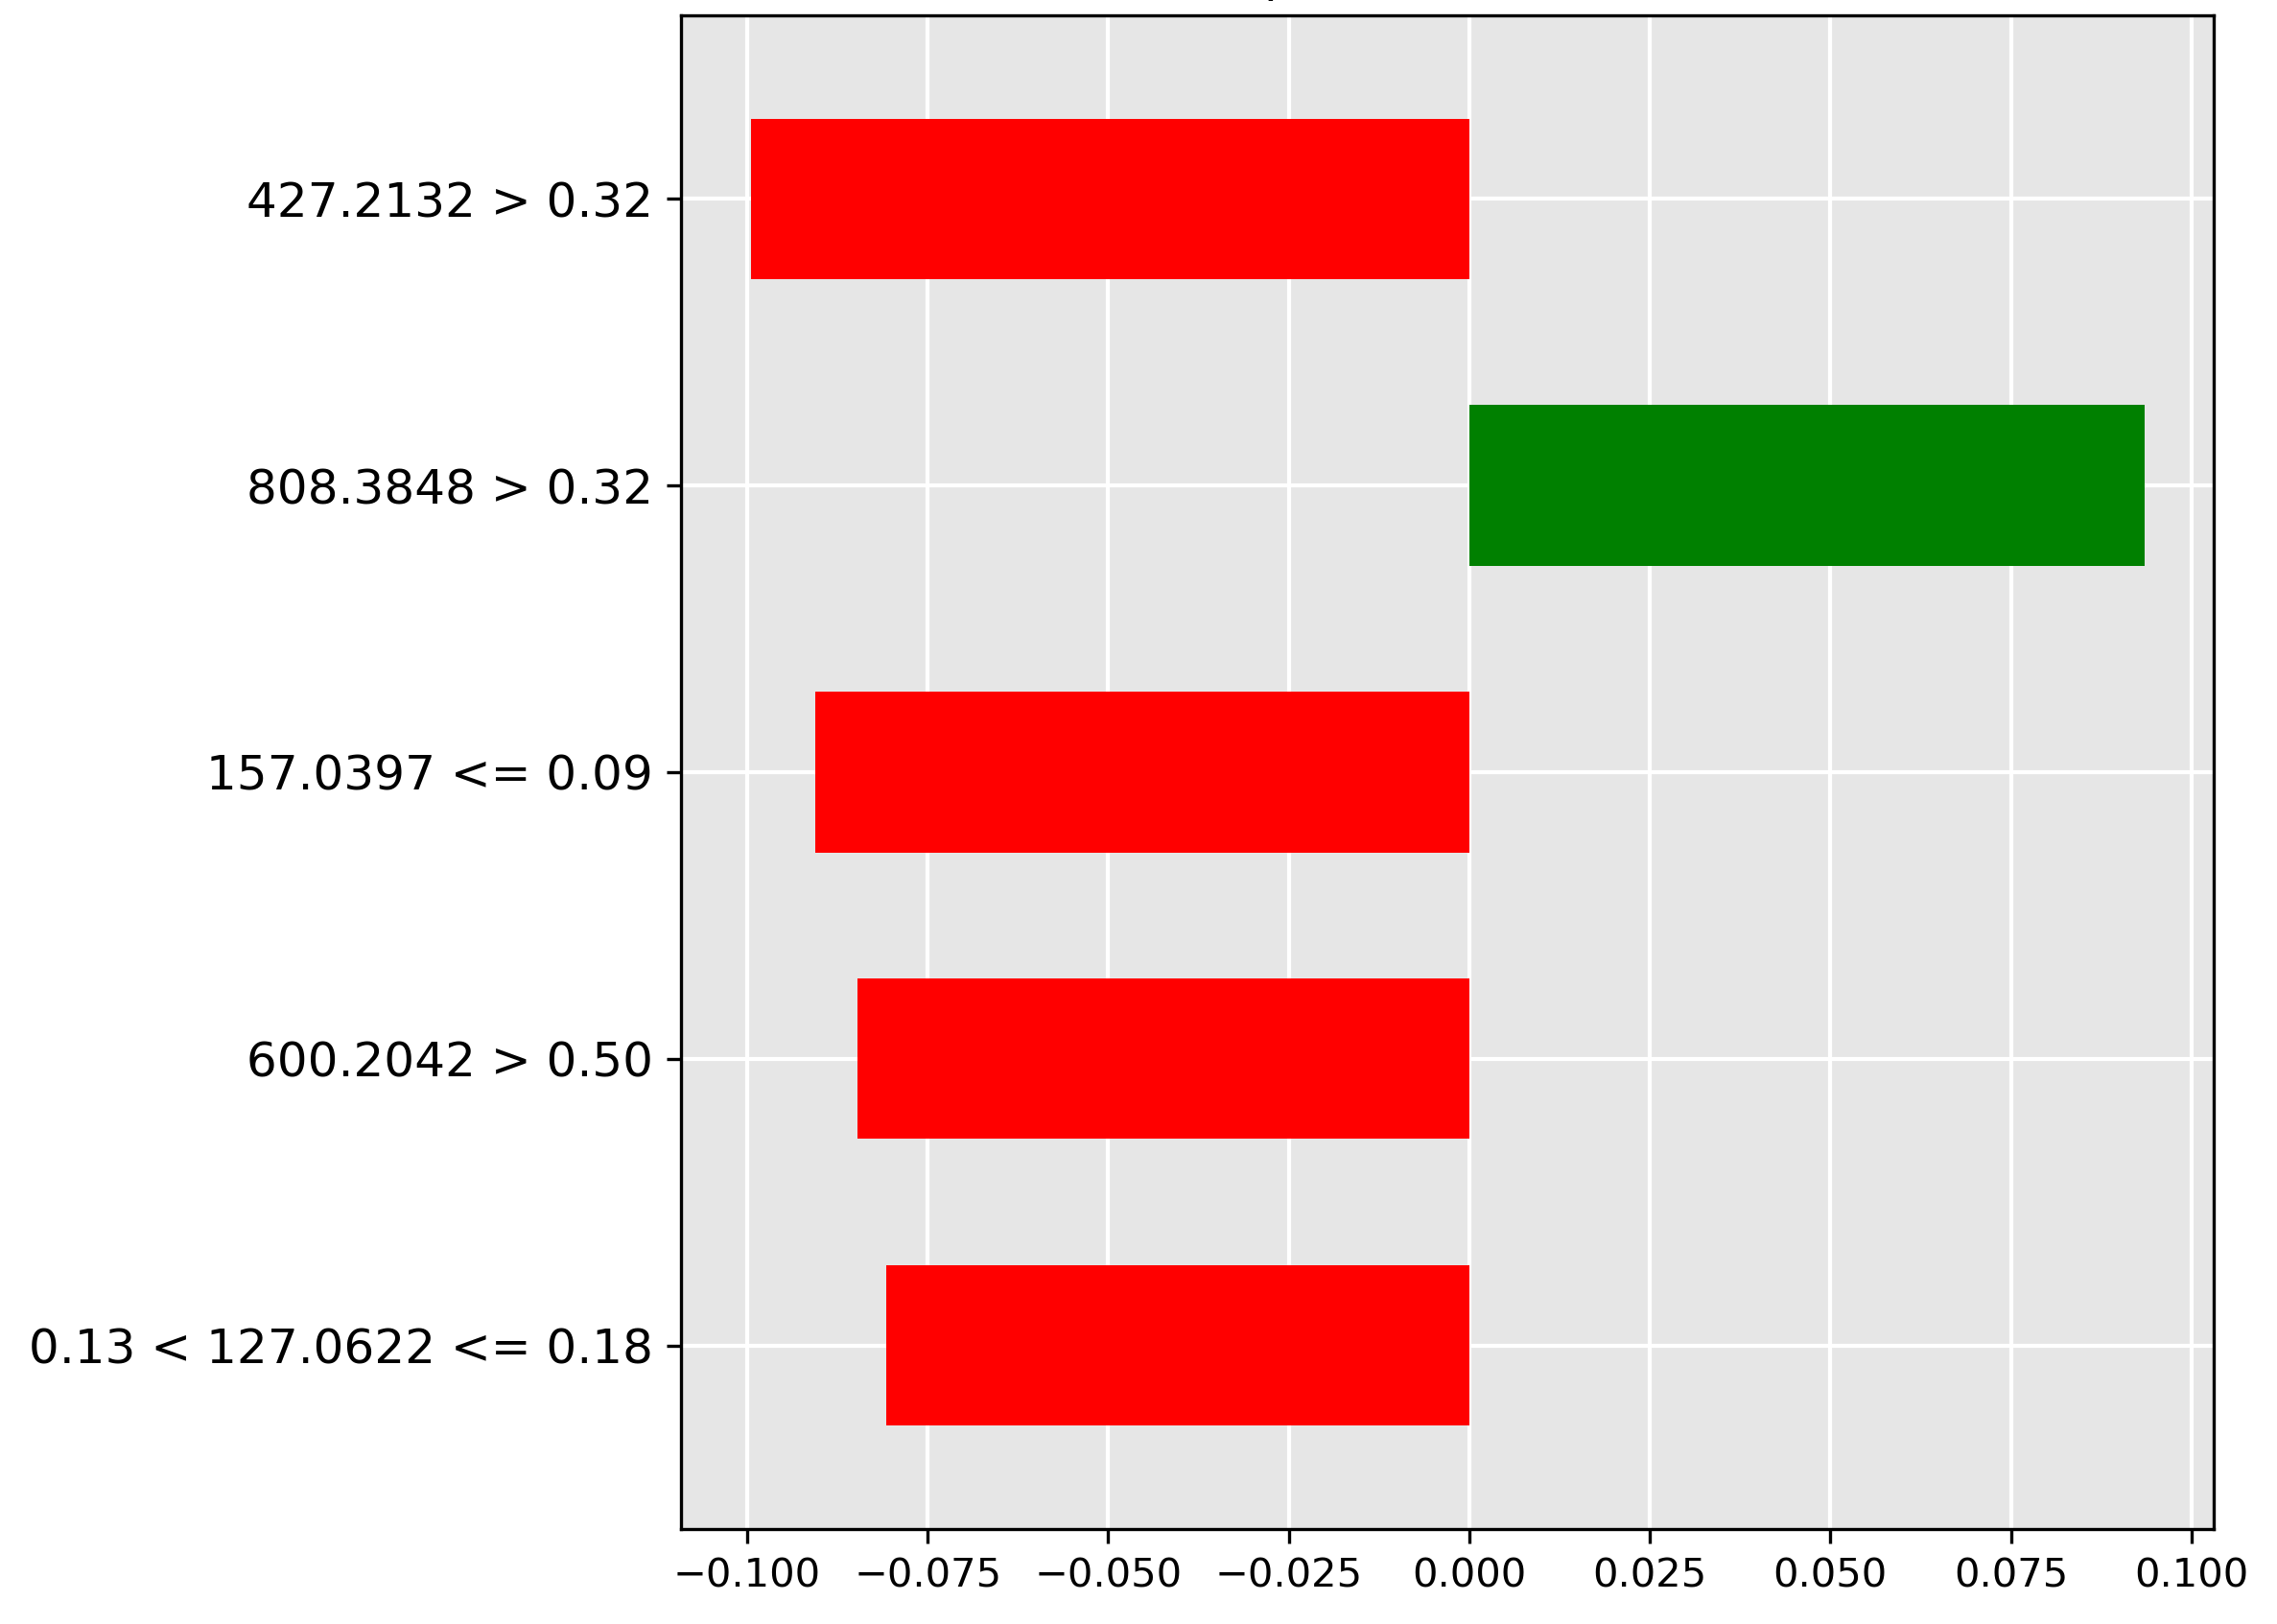
\includegraphics[width=0.7\linewidth]{assets/lime_transformer_cross-species_hoki-mackerel.png}
    \caption{LIME explanation for \textbf{pre-trained transformer} for cross-species contamination of \textbf{Hoki-Mackerel} class.}
    \label{fig:lime-transformer-cross-species-hoki-mackerel}
\end{figure}

For the \textbf{pure Hoki} class (\Cref{fig:lime-transformer-cross-species-hoki}), the strongest positive feature (green bar) is the high intensity ($> 0.09$) of the molecular ion $m/z~122.1110$. This feature is highly discriminant, indicating that the molecular ion is likely abundant exclusively in Hoki tissue.

\begin{figure}
    \centering
    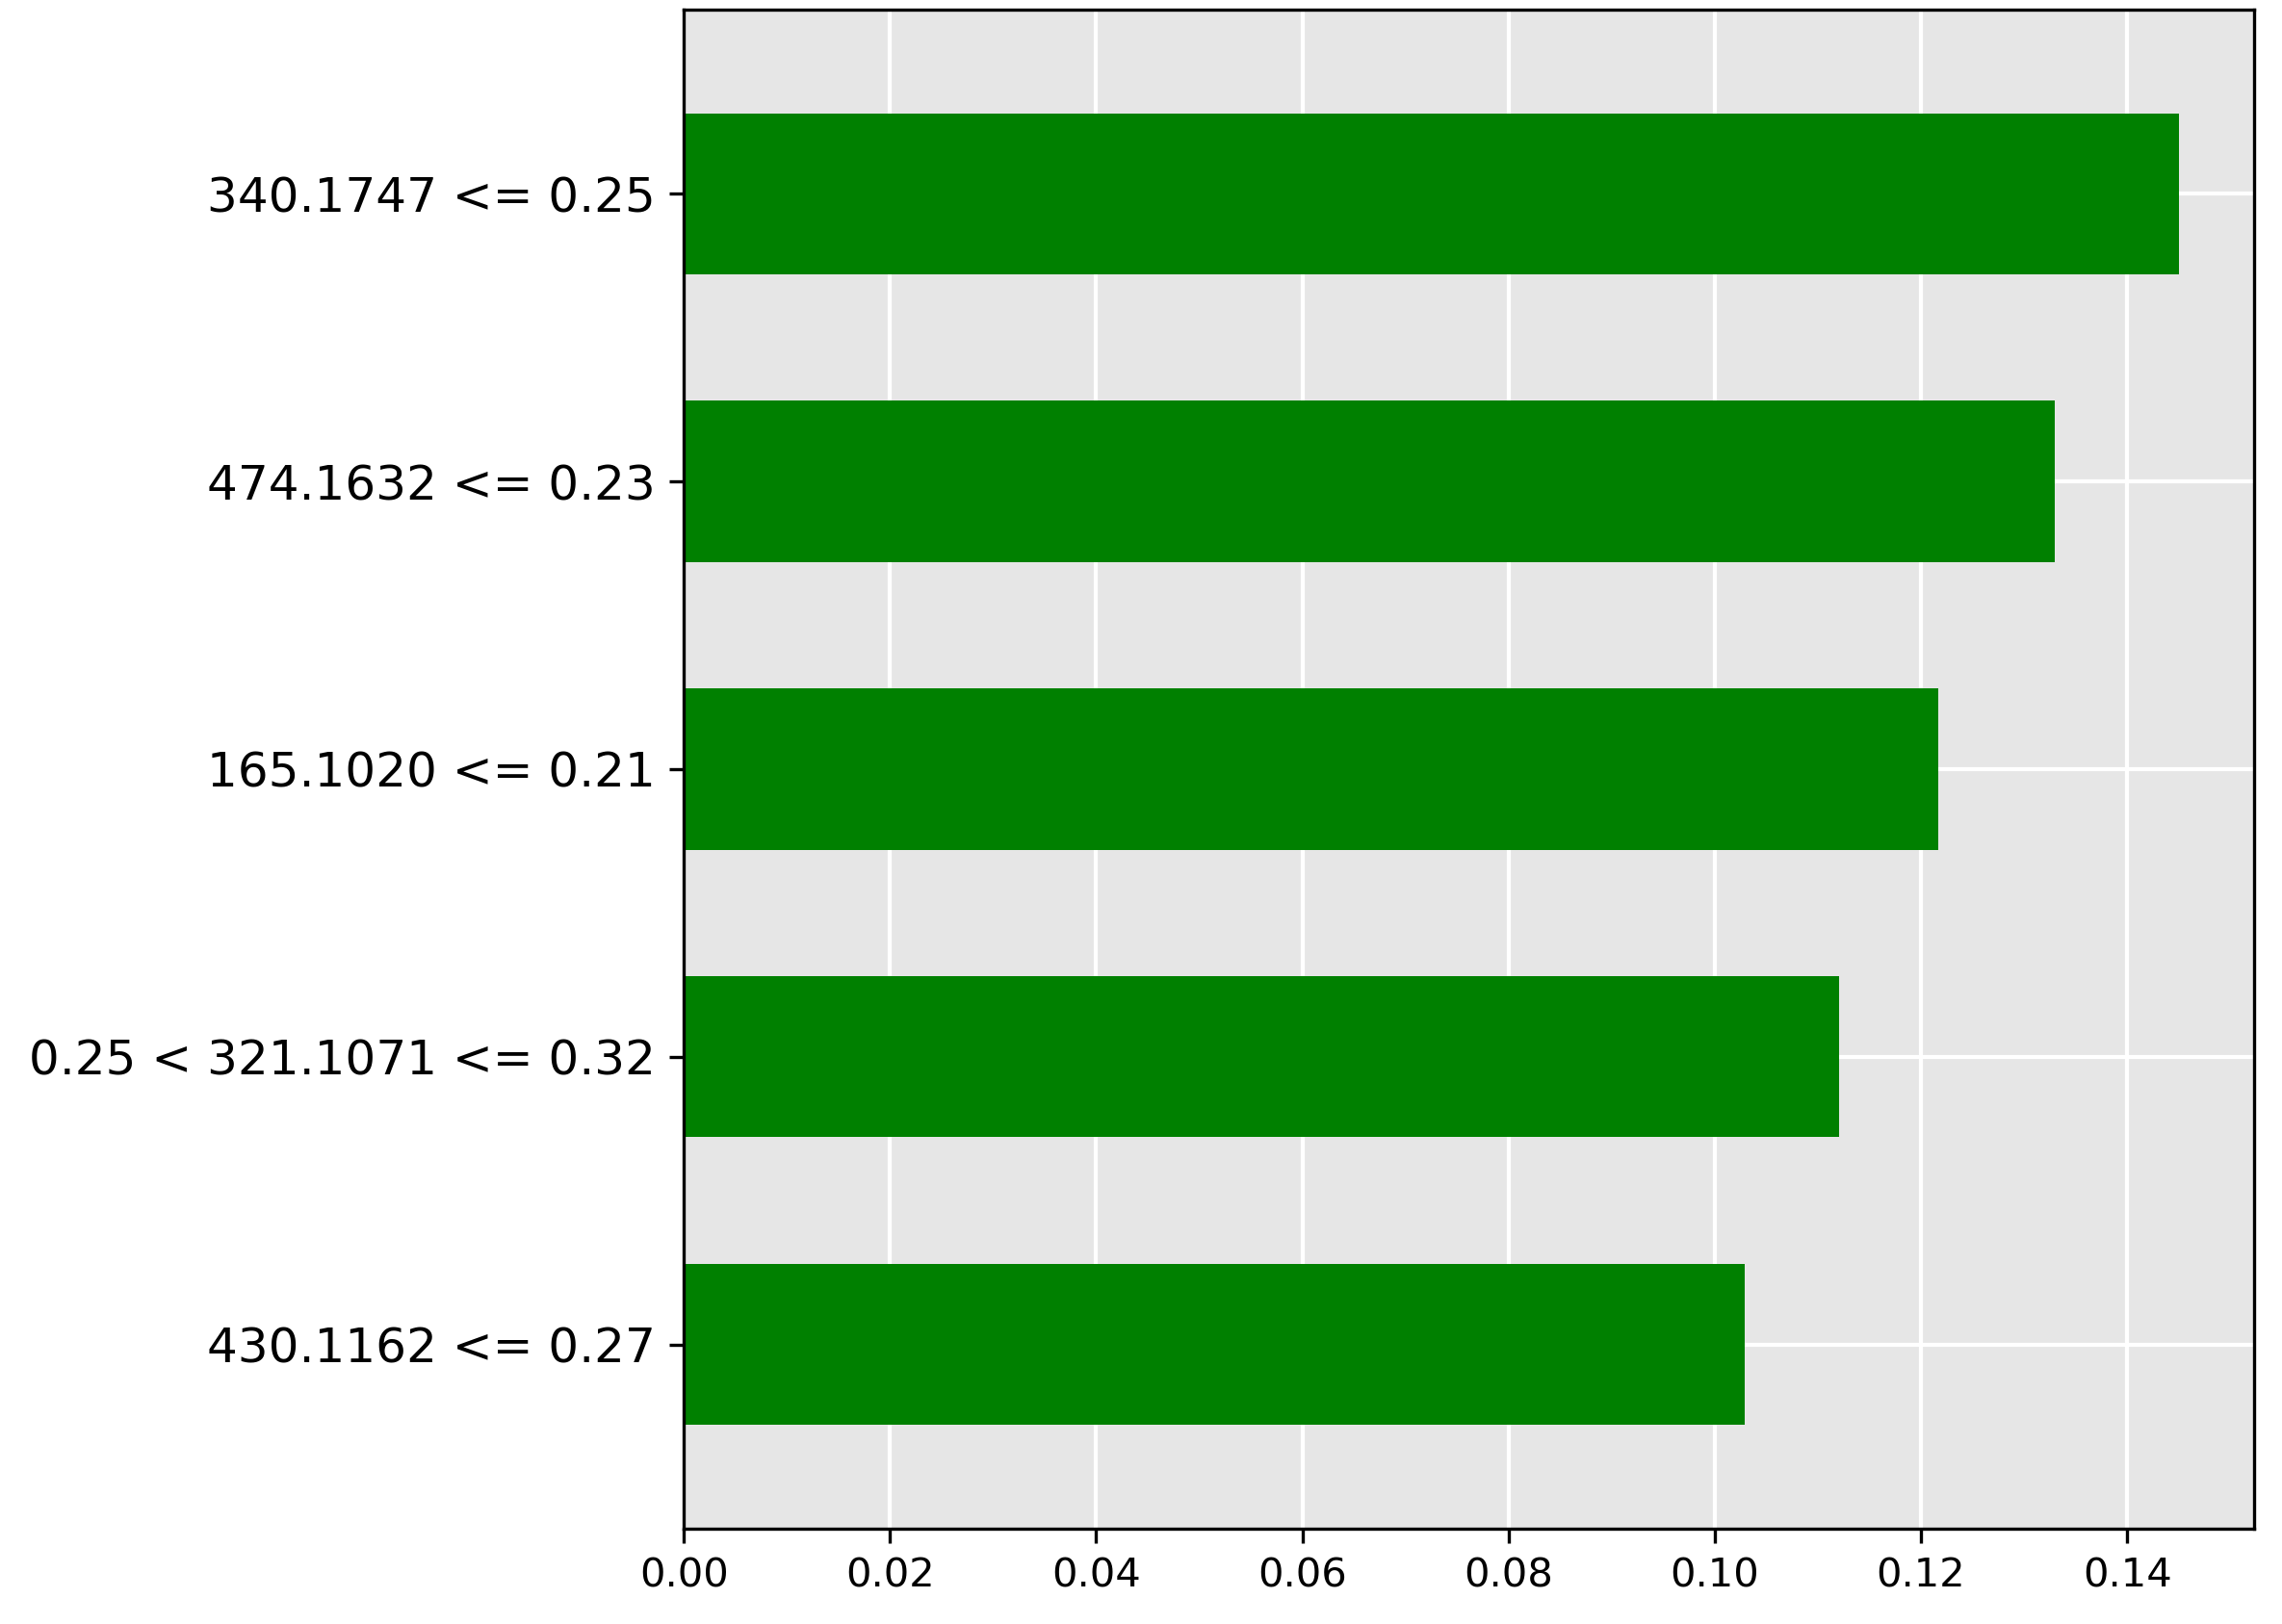
\includegraphics[width=0.7\linewidth]{assets/lime_transformer_cross-species_hoki.png}
    \caption{LIME explanation for \textbf{pre-trained transformer} for cross-species contamination of \textbf{Hoki} class.}
    \label{fig:lime-transformer-cross-species-hoki}
\end{figure}

Finally, the LIME explanation for the \textbf{pure Mackerel} class (\Cref{fig:lime-transformer-cross-species-mackerel}) shows the most important feature (red bar) is the very low intensity ($\le 0.07$) of the molecular ion $m/z~367.0835$. The model uses this low abundance to confirm the pure Mackerel classification; conversely, a higher abundance would suggest the presence of Hoki or the Hoki-Mackerel mix.

\begin{figure}
    \centering
    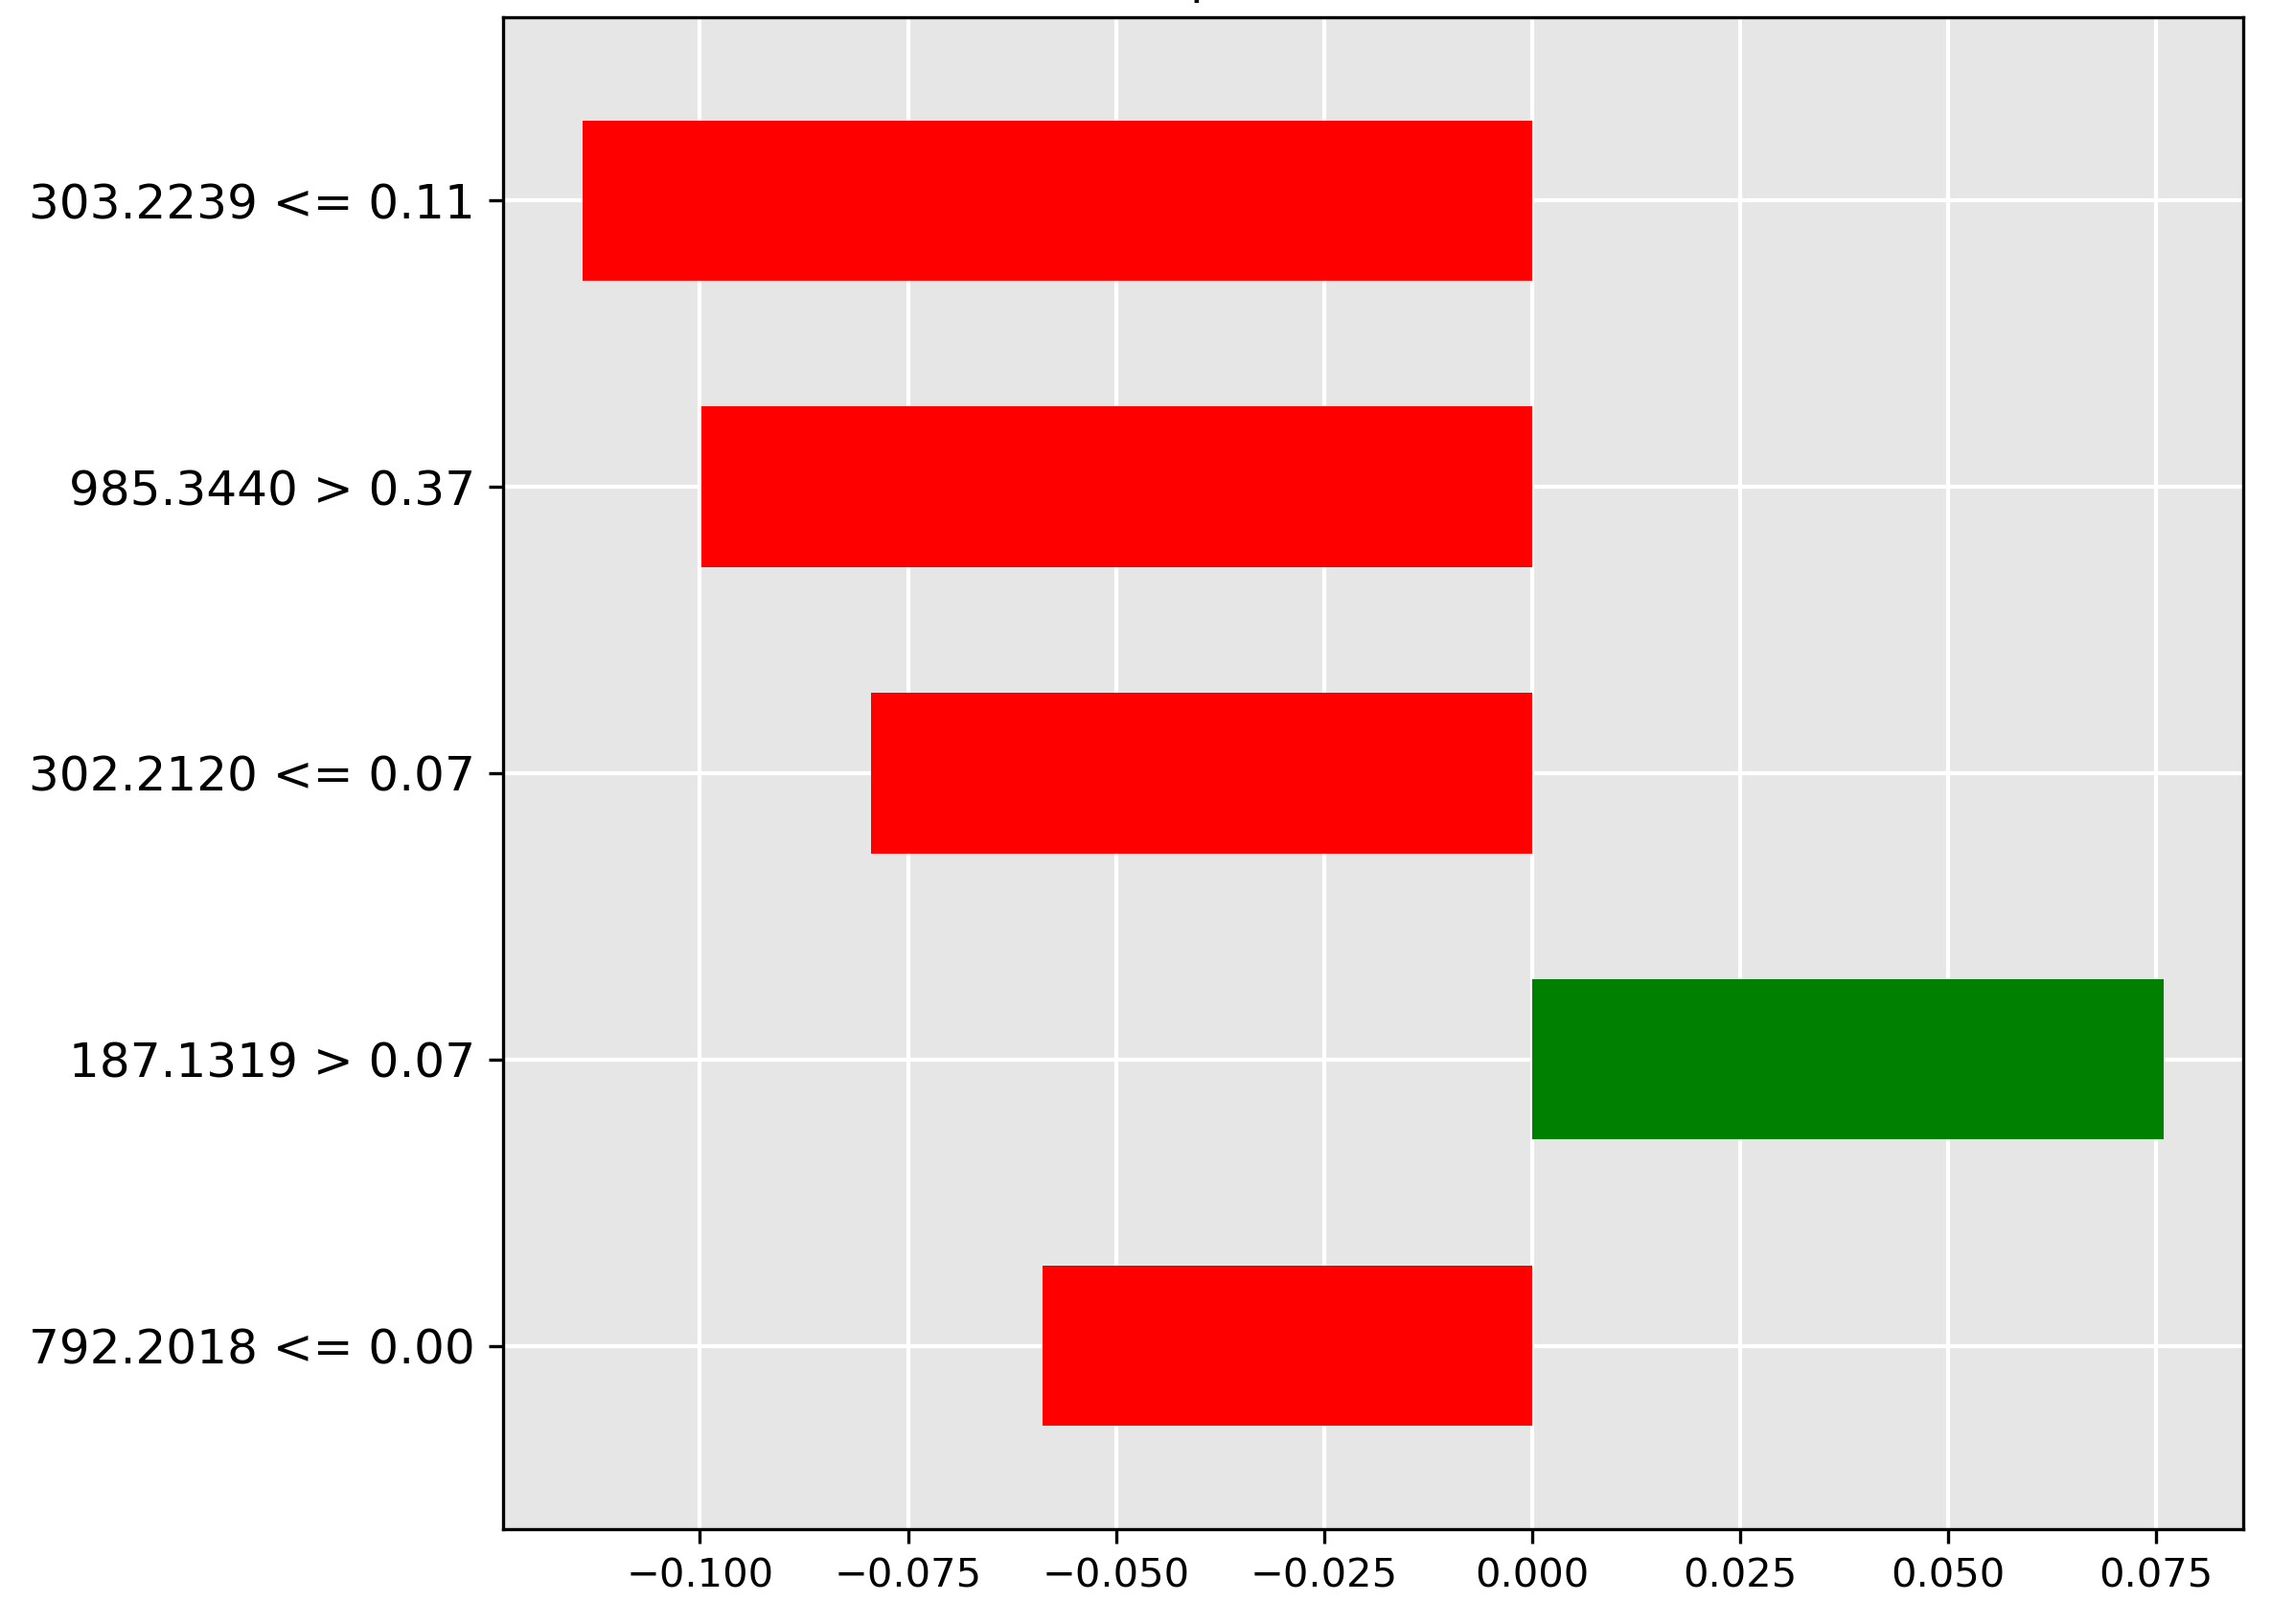
\includegraphics[width=0.7\linewidth]{assets/lime_transformer_cross-species_mackerel.png}
    \caption{LIME explanation for \textbf{pre-trained transformer} for cross-species contamination of \textbf{Mackerel} class.}
    \label{fig:lime-transformer-cross-species-mackerel}
\end{figure}

\subsubsection{Top 10 Features}

In this analysis, we analyze the top 10 features identified by 1D Grad-CAM for both classification tasks across four different models. \Cref{fig:top-features-oil} gives the top 10 features graph for oil contamination, and \Cref{fig:top-features-cross-species} gives the top 10 features graph for cross-species adulteration. There are two sets of trends that can be identified from these graphs: model-specific and task-specific.

For model-specific behavior, we identify trends in models that are shared across both classification tasks. For example, for both tasks, the LSTM chooses a tight cluster of features that are in a sequence. While the CNN, MoE, and Transformer choose a broader variety of feature subsets that span the entire mass-to-charge ratio range, except for the MoE for oil contamination. Each of the models chooses a different subset for its top 10 most important features. Similar to the previous chapter, this suggests that they form independent, complementary, and diverse models for an ensemble. This again motivates the use of an ensemble model.

For task-specific trends, we look for differences in the overall behavior of the models for each task. We notice that for oil contamination, the LSTM and MoE select a subset of features that are in the low range of mass-to-charge ratios ($\approx 100 - 500$). Whereas, for cross-species adulteration, the LSTM and MoE also utilize models from the mid to high range of mass-to-charge ratios ($\approx 600 - 1000$). This suggests that the lipids responsible for differentiating between different concentrations of oil contamination are mainly in the low range of mass-to-charge ratios. The lipids responsible for identifying cross-species adulteration between Hoki and Mackerel are in the mid-to-high ranges of mass-to-charge ratios. 

\begin{figure}
    \centering
    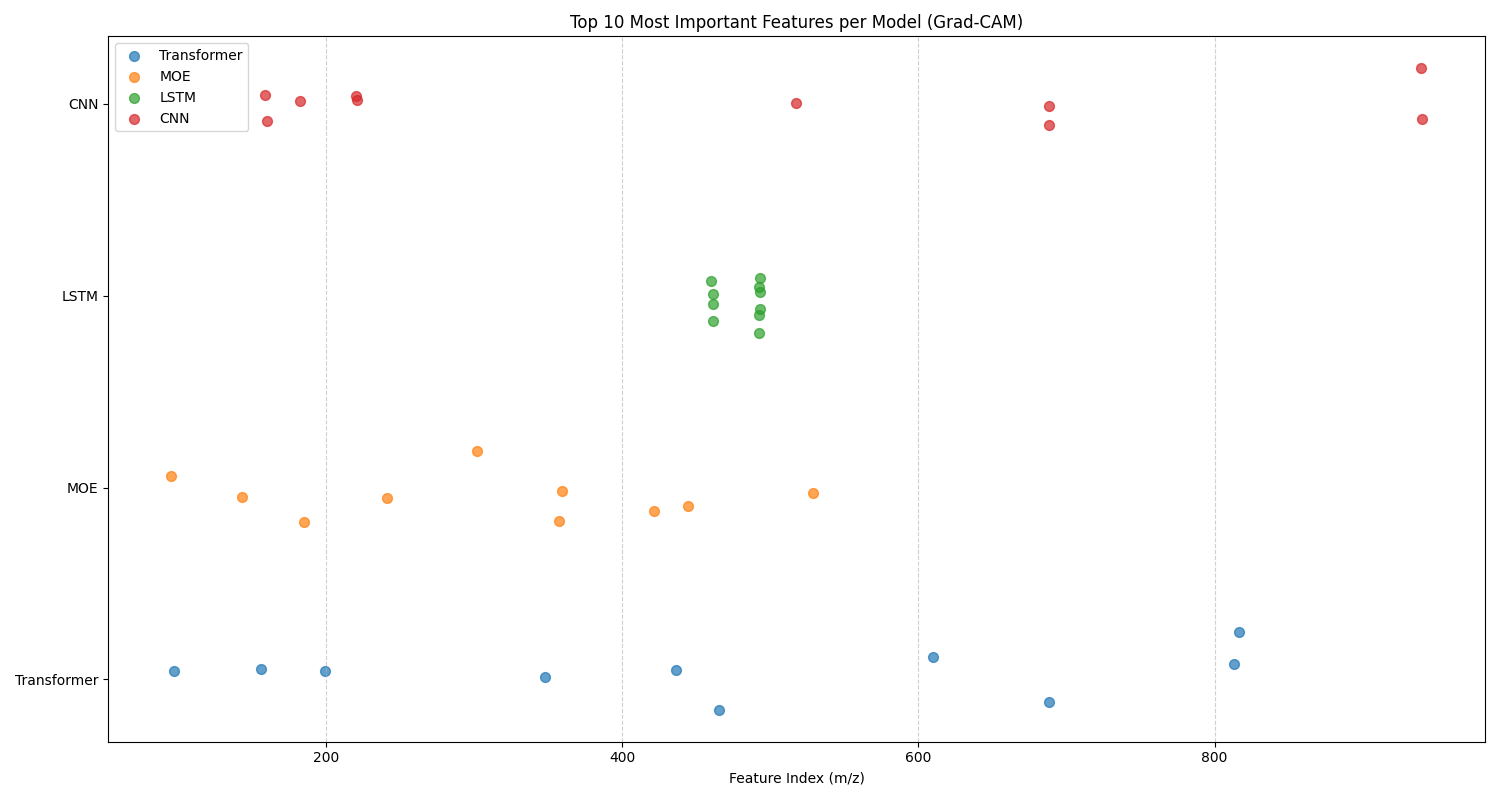
\includegraphics[width=\linewidth]{assets/top_features_comparison_oil.png}
    \caption{In this diagram, we present the top 10 features for \textbf{oil contamination} classification that have been identified by our 1D Grad-CAM analysis. We analyze the top 10 features for the CNN, LSTM, MOE, and Transformer models.}
    \label{fig:top-features-oil}
\end{figure}

\begin{figure}
    \centering
    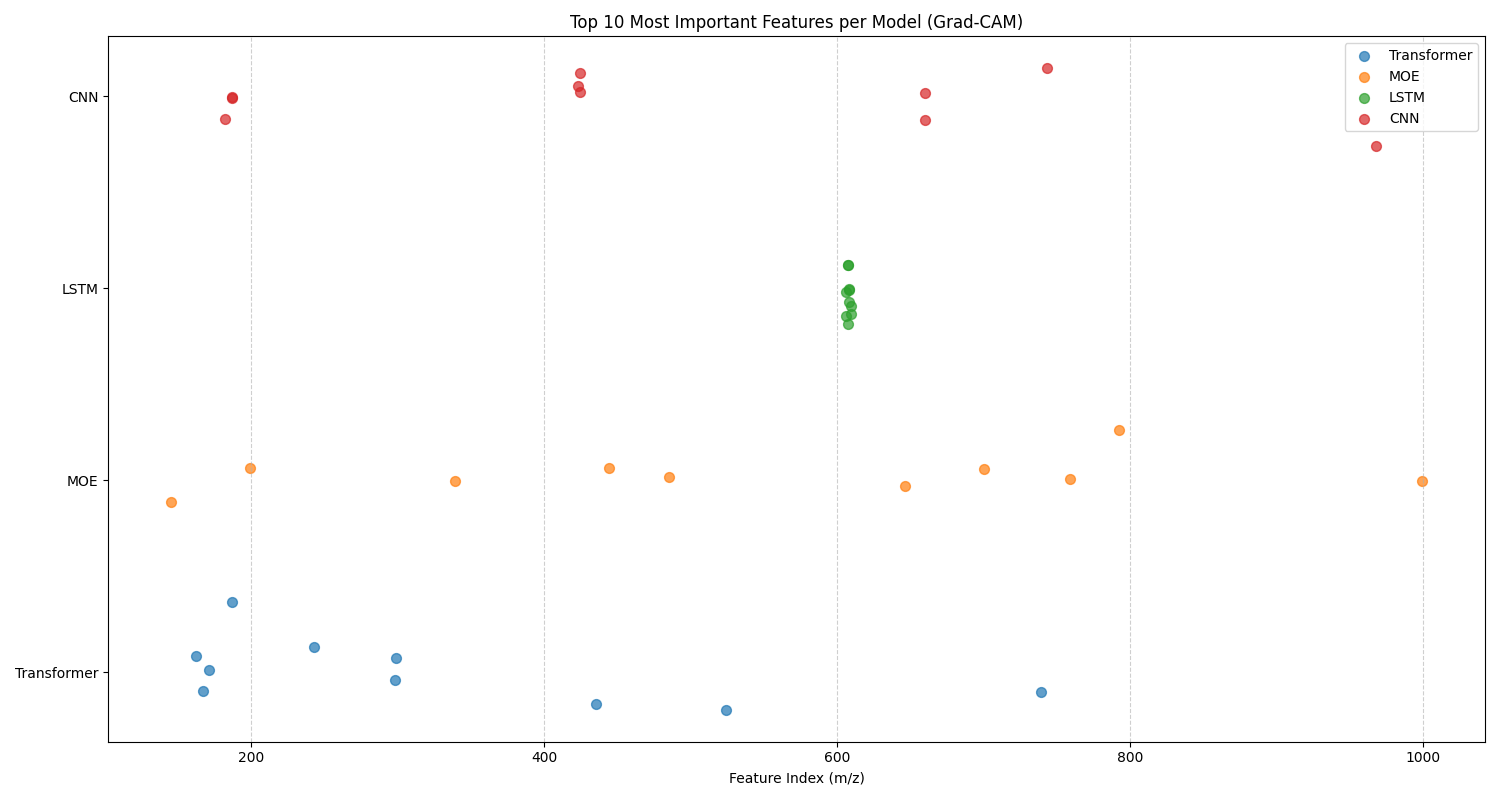
\includegraphics[width=\linewidth]{assets/top_features_comparison_cross-species.png}
    \caption{In this diagram, we present the top 10 features for fish \textbf{cross-species adulteration} classification that have been identified by our 1D Grad-CAM analysis. We analyze the top 10 features for the CNN, LSTM, MOE, and Transformer models.}
    \label{fig:top-features-cross-species}
\end{figure}

\subsection{Computational Cost}

\begin{table}
\small % Make the font size small to fit the printing area
\centering
\caption{Model Performance on Oil and Cross-Species Datasets.}
\label{tab:model_performance_oil_cs}
\begin{tabular}{llrrrc}
\toprule
Model & Dataset & Training Time (s) & Inference Time (s) & Model Size (MB) & Parameters \\
\midrule
Ensemble & cross-species & 3.0423 & 0.0272 & 976.1705 & 244042633 \\
Moe & cross-species & 0.3025 & 0.2415 & 77.9022 & 19475559 \\
Transformer & cross-species & 0.2069 & 0.0028 & 71.4527 & 17863171 \\
Pretrained & cross-species & 42.6161 & 0.0023 & 71.4527 & 17863171 \\
Ensemble & oil & 2.7665 & 0.0117 & 976.2704 & 244067605 \\
Moe & oil & 0.2820 & 0.1642 & 77.9355 & 19483883 \\
Transformer & oil & 0.1947 & 0.0025 & 71.4860 & 17871495 \\
Pretrained & oil & 30.2554 & 0.0023 & 71.4860 & 17871495 \\
\bottomrule
\end{tabular}
\end{table}

This computational cost benchmark evaluated our four transformer variants on the oil and cross-species datasets. We measured the training time, inference speed, model size in megabytes, and parameters. \Cref{tab:model_performance_oil_cs} lists this computational cost benchmark. Similar to the previous chapter, we see a striking convergence in inference time between the Transformer and Pretrained Transformer, while also illustrating the significant overhead associated with the more complex MoE and Ensemble Transformer models.

The parity in inference time between the standard Transformer and Pretrained Transformer exhibits fast and almost identical inference times. The extra time allocated for pretraining is shown in the large differences in the training time column. In stark contrast, the more complex architectures demonstrate clear performance trade-offs. The Ensemble model, while achieving fast inference, requires a training time more than ten times longer than simpler transformers. Reflecting the linear cost of training multiple models. The MoE architecture is a notable outlier,  delivering the slowest inference speeds by a massive margin—nearly 100 times slower than the standard Transformer. This result strongly indicates that for models of this scale, the computational overhead of the MoE's expert-routing mechanism provides no benefit and instead introduces a significant performance bottleneck.

Ultimately, this analysis underscores that optimization is king. The benchmark shows that a well-optimized, standard Transformer architecture provides an outstanding balance of rapid training and exceptionally fast inference. The similar performance of the from-scratch and pretrained models suggests that the final optimization process is the dominant factor in determining runtime speed. For developers working with these datasets, the data indicates that architectural complexity should be approached with caution, as a simple, efficiently compiled model offers the most direct path to high performance.

Expert utilization, shown in \Cref{fig:expert-utilization,fig:expert-utilization-radar}, is balanced across tasks, indicating effective model capacity use without expert collapse.

\begin{figure}
    \centering
    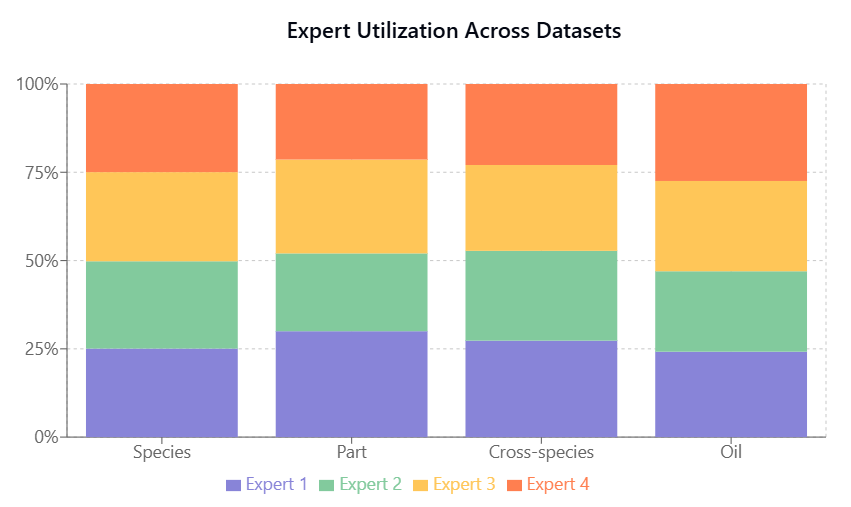
\includegraphics[width=0.7\linewidth]{assets/expert_utilization.png}
    \caption{This stacked bar chart shows the expert utilization of the MoE Transformer with 4 experts across all four classification tasks. We see balanced expert utilization across all tasks, indicating that the model does not suffer from expert collapse, where one or more experts are hardly used or redundant in training and inference.}
    \label{fig:expert-utilization}
\end{figure}

\begin{figure}
    \centering
    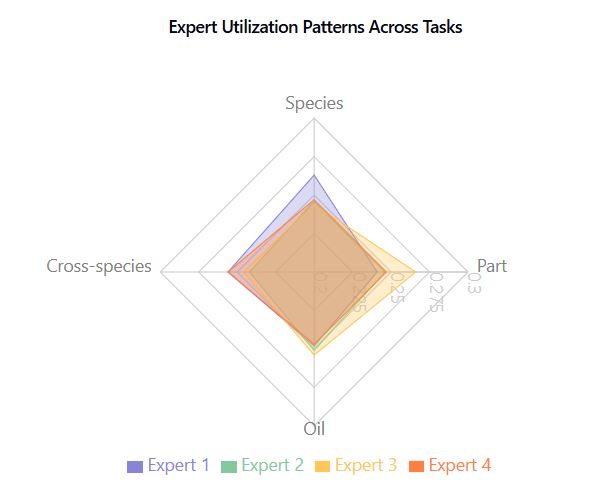
\includegraphics[width=0.7\linewidth]{assets/expert_utilization_radar.png}
    \caption{This radar chart illustrates the utilization patterns of four different experts across four task categories: Species, Part, Oil, and Cross-species.}
    \label{fig:expert-utilization-radar}
\end{figure}

\subsection{Ablation of MoE Transformer}
\label{sec:ablation-studies}

After analyzing the comparative performance of the routing strategies, we conducted a series of ablation studies to better understand the architectural choices in our MoE Transformer and their impact on the model performance. These studies systematically examine the effects of majority voting versus Top-k routing, expert count, and Top-k routing values, providing insights into the model's behavior and optimal configuration for different classification tasks.

\subsubsection{Majority Voting versus Top-k Routing:}
We compared two MoE routing strategies: Top-k routing (dynamically routes inputs to k=2 most relevant experts) and majority voting (processes inputs through all experts and averages outputs). Each variant was tested across four classification tasks with 5 runs per configuration.

\begin{table}[!t]
\caption{Top-k Routing versus Majority Voting}
\label{tab:routing-results-chp5}
\centering
\begin{tabular}{@{}lcc@{}}
\toprule
Dataset & Top-k Routing & Majority Voting \\
\midrule
Cross-species & \textbf{88.04 $\pm$ 4.84} & 87.56 $\pm$ 1.10  \\
Oil & \textbf{45.51 $\pm$ 5.60} & 43.65 $\pm$ 0.53 \\
\bottomrule
\end{tabular}
\end{table}

As shown in \Cref{tab:routing-results-chp5}, and \Cref{fig:routing-bar-chart-chp5} Top-k Routing achieved higher accuracy across all tasks, but with greater variance. Majority Voting demonstrated more consistent predictions with lower standard deviations, aligning with previous research \citep{Suzuoki2024}. Both methods performed poorly on oil contamination detection ($<$ 46\% accuracy), suggesting this task requires further architectural improvements beyond routing strategy modifications.

\begin{figure}
    \centering
    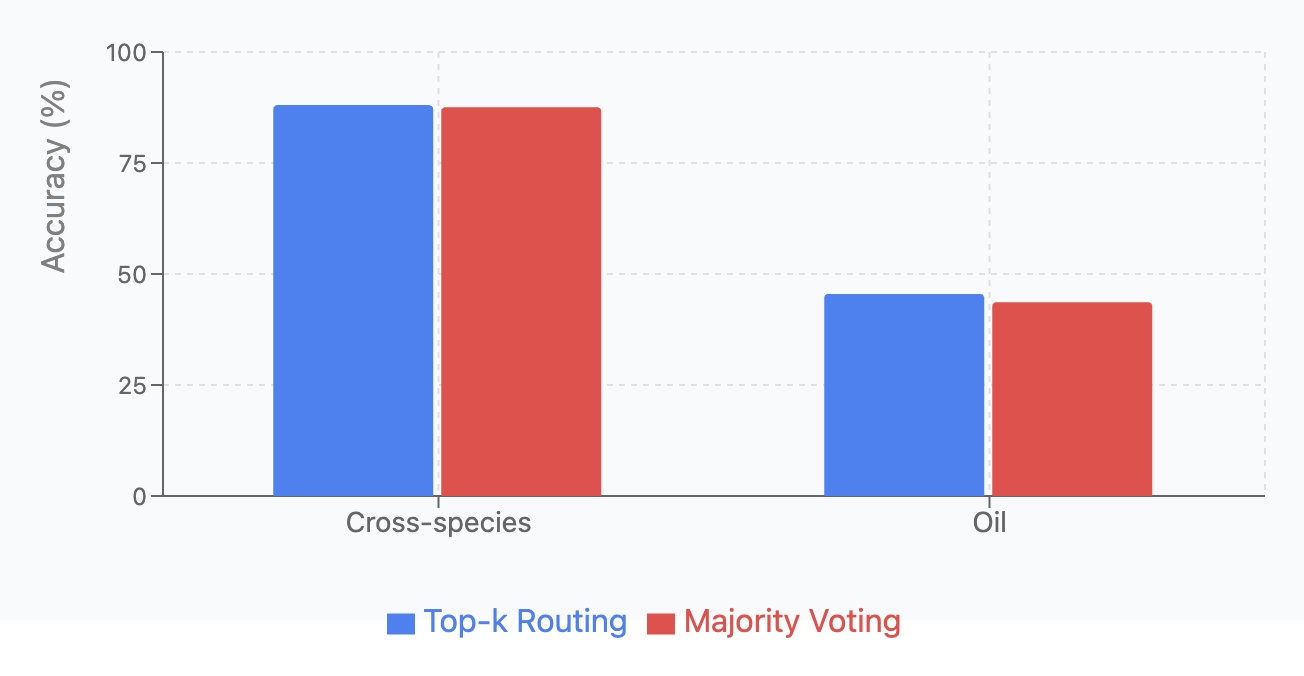
\includegraphics[width=0.7\linewidth]{assets/routing_accuracy_bar_chart_ch-5.png}
    \caption{Majority Voting versus Top-k Routing Bar Chart}
    \label{fig:routing-bar-chart-chp5}
\end{figure}

\subsubsection{Expert Count Analysis:}

We tested model performance with different numbers of experts (E=2, 4, 8) across four classification tasks, running each variant 5 times. Results are shown in \Cref{tab:expert-count-analysis-chp5} and \Cref{fig:expert-bar-chart-chp5}.

\begin{table}[!t]
\caption{Expert Count Analysis}
\label{tab:expert-count-analysis-chp5}
\centering
\begin{tabular}{@{}lccc@{}}
\toprule
Dataset & $E=2$ & $E=4$ & $E=8$ \\
\midrule
Cross-species & \textbf{88.87 $\pm$ 1.17} & 88.04 $\pm$ 4.84 & 87.82 $\pm$ 1.29 \\ 
Oil & 45.37 $\pm$ 1.35 & \textbf{45.51 $\pm$ 5.60} & 43.75 $\pm$ 1.69 \\
\bottomrule
\end{tabular}
\end{table}

Key findings: 
(1) Cross-species contamination showed stable performance (87-89\%) across all configurations; 
(2) Oil contamination detection was consistently difficult (43-45\%) regardless of expert count; 
(3) E=4 provides the best balance between specialization capacity and ensuring sufficient training data per expert.

\begin{figure}
    \centering
    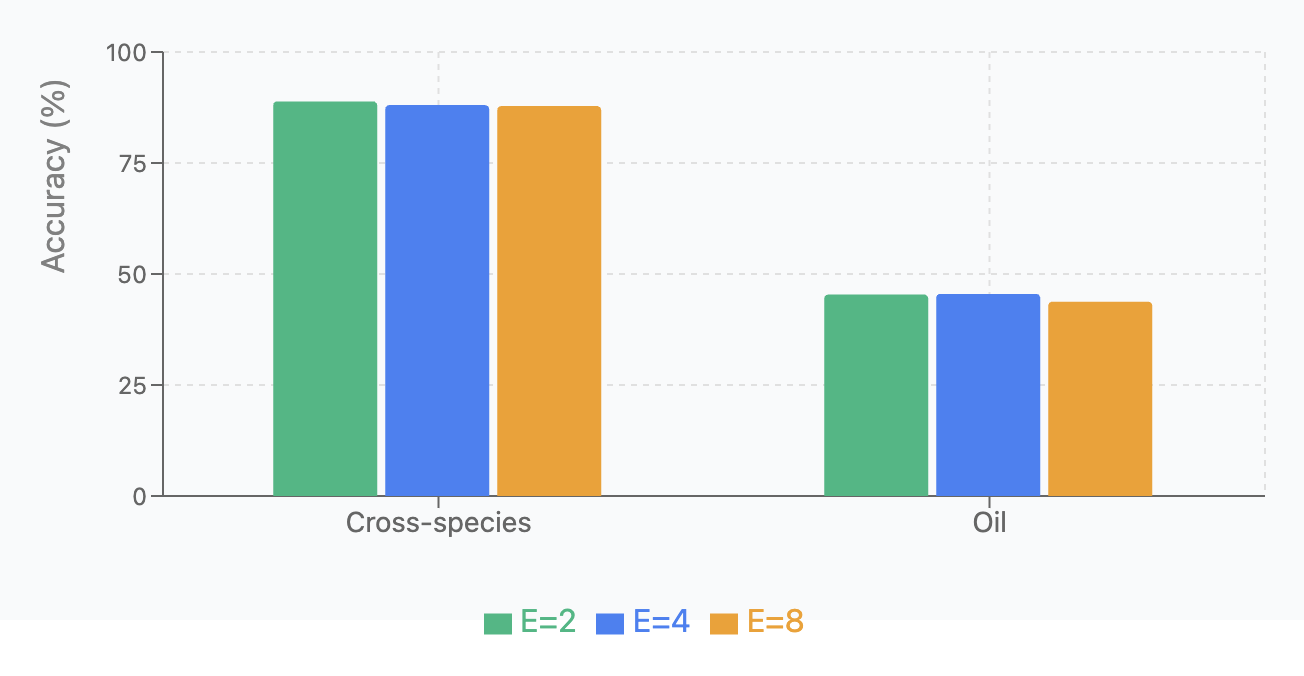
\includegraphics[width=0.7\linewidth]{assets/expert_count_analysis_ch_5.png}
    \caption{Expert Count Analysis Bar Chart}
    \label{fig:expert-bar-chart-chp5}
\end{figure}

\subsubsection{Top-k Routing:}

We compared performance with different k values (1, 2, 4) across the same four tasks, using the same experimental setup. Results are shown in \Cref{tab:topk-routing-chp5} and \Cref{fig:topk-bar-chart-chp5}.

\begin{table}[!t]
\caption{Top-k Routing}
\label{tab:topk-routing-chp5}
\centering
\begin{tabular}{@{}lccc@{}}
\toprule
Dataset & $k=1$ & $k=2$ & $k=4$ \\
\midrule
Cross-species & 89.27 $\pm$ 0.89 & 88.04 $\pm$ 4.84 & \textbf{89.93 $\pm$ 1.82} \\ 
Oil & \textbf{45.69 $\pm$ 1.78} & 45.51 $\pm$ 5.60 & 45.38 $\pm$ 1.14 \\
\bottomrule
\end{tabular}
\end{table}

Key findings: 
(1) k=4 was optimal for cross-species detection, suggesting benefit from broader expert consultation; 
(2) Oil contamination showed similar performance across all k values (~45\%); 
(3) Overall, k=2 provides the best balance between specialization and redundancy for most tasks.

\begin{figure}
    \centering
    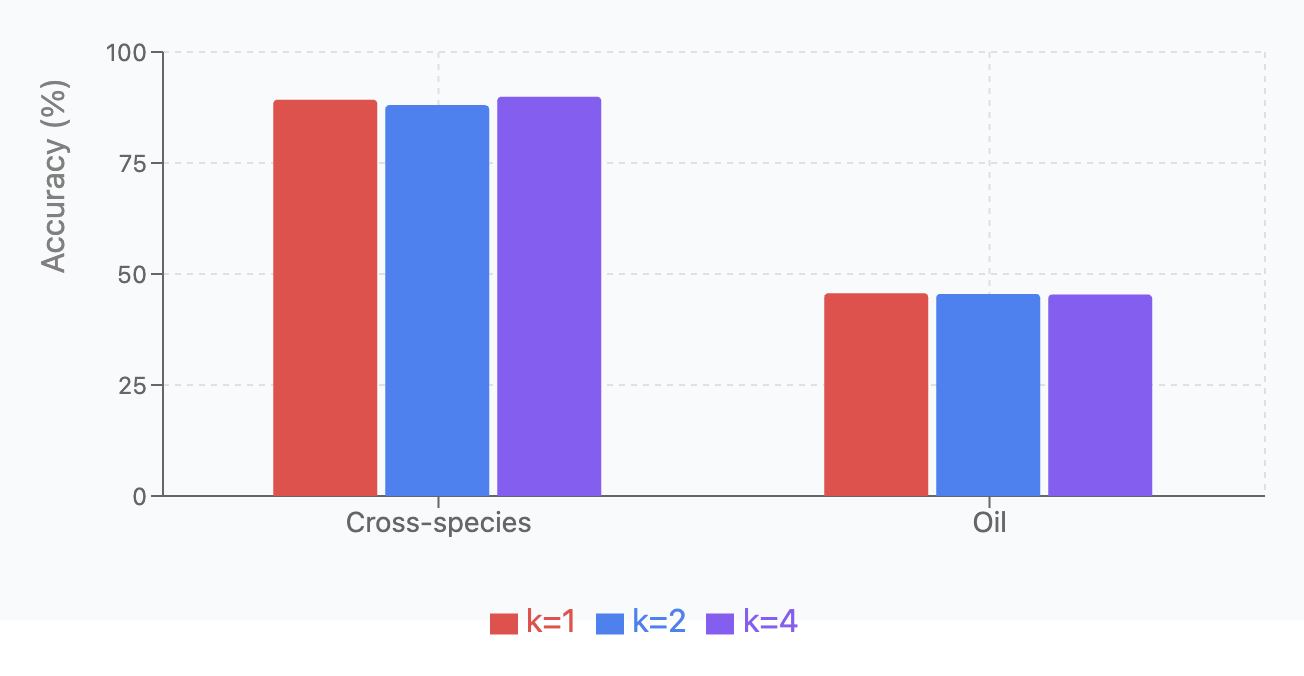
\includegraphics[width=0.7\linewidth]{assets/topk_routing_chp_5.png}
    \caption{Top-k Routing Bar Chart}
    \label{fig:topk-bar-chart-chp5}
\end{figure}

\subsection{Ablation of Transfer Learning}

After the description of the experimental design, the Results section presents the empirical findings and analyzes the observed patterns in transfer learning effectiveness across different fish fraud detection tasks. This section is broken down into discussions on Overall Performance and Asymmetric Transfer Effects, the Impact of Task Difficulty on Transfer Learning, the Role of Model Architecture (MoE Transformer), Model Stability and Standard Deviations, and Practical Implications and Resource Allocation.

\begin{table}[!t]
\caption{Transfer Learning Results on Test Set (\%) with Standard Deviations}
\label{tab:transfer_results}
\centering
\begin{tabular}{@{}lccc@{}}
\toprule
Source $\rightarrow$ Target & Baseline & Transfer & Effect \\
\midrule
Oil $\rightarrow$ Cross-species & 88.04\% $\pm$ 4.84\% & 83.44\% $\pm$ 6.91\% & - \\
Species $\rightarrow$ Oil & 45.51\% $\pm$ 5.60\% & 46.28\% $\pm$ 6.84\% & + \\
Part $\rightarrow$ Oil & 45.51\% $\pm$ 5.60\% & 45.64\% $\pm$ 7.21\% & + \\
Cross-species $\rightarrow$ Oil & 45.51\% $\pm$ 5.60\% & 49.10\% $\pm$ 5.85\% & + \\
\bottomrule
\end{tabular}
\end{table}

\begin{figure*}
    \centering
    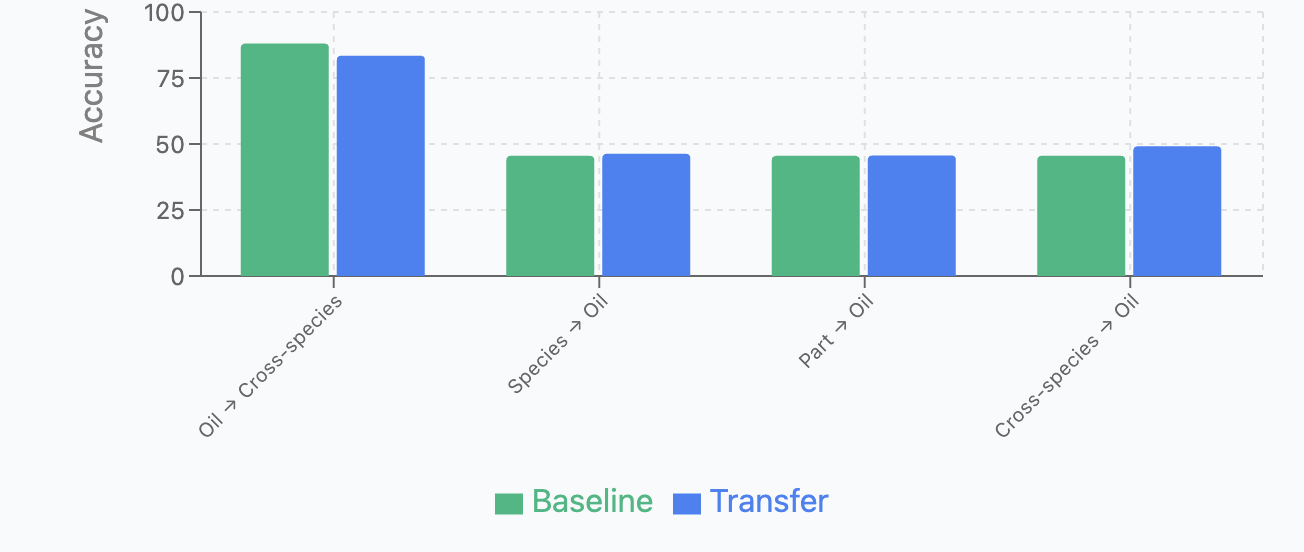
\includegraphics[width=\linewidth]{assets/improvements_bar_chart_ch_5.png}
    \caption{Test Classification Improvements Bar Chart: This bar chart illustrates the performance (\%) of Baseline (blue) versus Transfer Learning (green) models on six different classification scenarios: Oil → Cross-species, Species → Oil, Part → Oil, and Cross-species → Oil. Error bars indicate the variability in performance. }
    \label{fig:improvements-bar-chart}
\end{figure*}

\begin{figure}
    \centering
    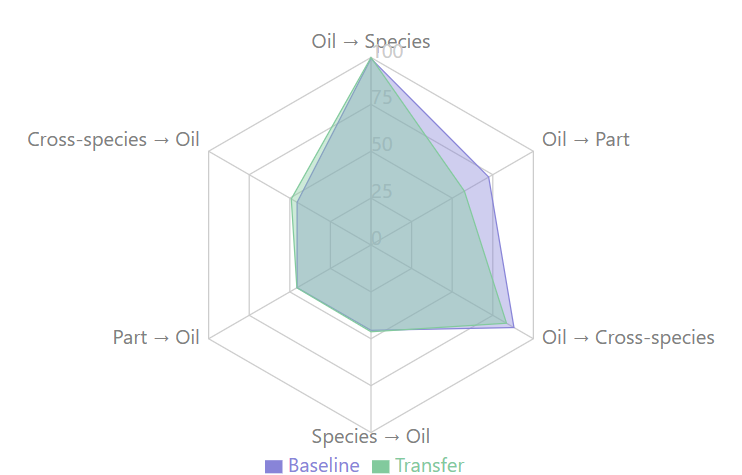
\includegraphics[width=0.8\linewidth]{assets/transfer_radar.png}
    \caption{Test Classification Improvements Radar Chart: This radar chart provides a comparative view of Baseline (green) and Transfer Learning (blue) model performance (in percentages) across six distinct classification tasks: Oil → Species, Oil → Part, Oil → Cross-species, Species → Oil, Part → Oil, and Cross-species → Oil. }
    \label{fig:improvements-radar-chart}
\end{figure}

\subsubsection{Overall Performance and Asymmetric Transfer Effects}

The experimental results, with performance metrics averaged over 30 independent runs, are detailed in \Cref{tab:transfer_results}. A visual comparison of baseline and transfer learning performance across six source-target pairs is presented in the bar chart in \Cref{fig:improvements-bar-chart}. This chart displays accuracy percentages, with blue bars for baseline performance, green bars for transfer learning results, and error bars indicating standard deviations. The visualization reveals mixed outcomes: 
the Oil → Species transfer achieves perfect accuracy (100\%) with no improvement over its baseline;
Oil → Part and Oil → Cross-species show notable performance declines (dropping from 72.46\% to 57.50\% and 88.04\% to 83.44\%, respectively);
while the three ``→ Oil" transfers (Species → Oil, Part → Oil, Cross-species → Oil) demonstrate modest improvements over their common baseline of 45.51%.

Further illustrating these dynamics, the radar chart in \Cref{fig:improvements-radar-chart} depicts transfer learning performance across the same six source-target pairs. This chart uses overlapping polygons for baseline accuracy (purple) and transfer accuracy (green), allowing direct comparison. Areas where the green polygon extends beyond the purple signify improvements, while recession indicates degradation.
The three transfers targeting oil contamination detection (``→ Oil") show modest improvements, with Cross-species → Oil achieving the largest gain (+3.59\%).

The experimental results highlight a striking asymmetry in the effectiveness of transfer learning across the different fish fraud detection tasks. 
Transfer learning consistently improves oil contamination detection accuracy by modest yet meaningful margins (between 0.13\% and 3.59\%), irrespective of the source domain used for pre-training. 
Conversely, 
Transfer learning substantially degrades performance when applied to fish body part identification, 
With accuracy dropping by 14.96\% when transferring from oil contamination detection. 
Similarly, cross-species adulteration detection suffers a notable decline of 4.60\% when knowledge is transferred from oil contamination detection. 
These patterns suggest that the target domain, rather than the source domain, is the primary determinant of transfer learning success in this context.

\subsubsection{Impact of Task Difficulty on Transfer Learning}

Interestingly, the most difficult task, oil contamination detection (baseline accuracy of 45.51\%), consistently benefited from transfer learning regardless of the source domain. In contrast, easier tasks, such as fishy body part identification (72.46\% baseline) and cross-species adulteration detection (88.04\% baseline), were consistently harmed by transfer learning. This observation contradicts the intuitive expectation that easier tasks might derive greater benefit from knowledge transfer. A potential explanation for this phenomenon is that the chemical signatures detected for oil contamination may represent fundamental molecular patterns that are enhanced by exposure to diverse fish tissue data. Conversely, the specific features distinguishing different fish parts or identifying cross-species adulteration might be more specialized and could be confounded by knowledge transfer from other domains.

\subsubsection{Role of Model Architecture (MoE Transformer)}

The choice of a Mixture of Experts (MoE) transformer architecture may partially explain these results. The MoE approach facilitates the specialization of different experts on various aspects of the data, potentially creating a more modular knowledge representation. When transferring to the oil contamination detection task, this modularity might enable the model to retain and build upon relevant chemical pattern recognition capabilities while discarding irrelevant information. However, when transferring to fish body part identification or cross-species adulteration detection, the pre-trained experts may have developed specializations that conflict with the target task requirements, leading to negative transfer. The gating network's routing mechanism, which determines expert engagement for given inputs, might necessitate substantial retraining to adapt effectively to these tasks, thereby rendering transfer learning less effective than training from scratch.

\subsubsection{Model Stability and Standard Deviations}

The standard deviations observed in the results offer important insights into model stability across different transfer scenarios. All transfers targeting oil contamination detection shared a similar baseline performance (45.51\% ±5.60\%) but displayed varying degrees of improvement and stability; notably, the Cross-species → Oil transfer demonstrated the most substantial and consistent improvement, achieving 49.10\% ±5.85\%.

\subsubsection{Practical Implications and Resource Allocation}

From a practical standpoint, these findings carry significant implications for the development and deployment of automated quality control systems in the seafood processing industry. The computational overhead associated with transfer learning must be carefully weighed against the potential performance gains, which, as the results suggest, are highly task-dependent. For oil contamination detection, investing in transfer learning appears to be a worthwhile endeavour, potentially improving detection accuracy by up to 3.59\% when knowledge is transferred from the cross-species domain. This nuanced understanding of when and where to apply transfer learning can effectively guide resource allocation in real-world deployment scenarios, thereby optimizing both computational efficiency and detection accuracy in fish fraud prevention systems.

\subsection{Ordinal Classification} 

The oil contamination task, with its seven ordered concentration levels (0\% to 50\%), is a classic example of an ordinal classification problem. As illustrated in Figure \ref{fig:data_types}, ordinal data is distinct from nominal data (which has no order) and metric data (which assumes equidistant intervals). This inherent order---where a 5\% concentration is closer to 1\% than to 50\%---is critical information that standard classification or regression models may fail to capture.

\begin{figure}[htbp]
  \centering
  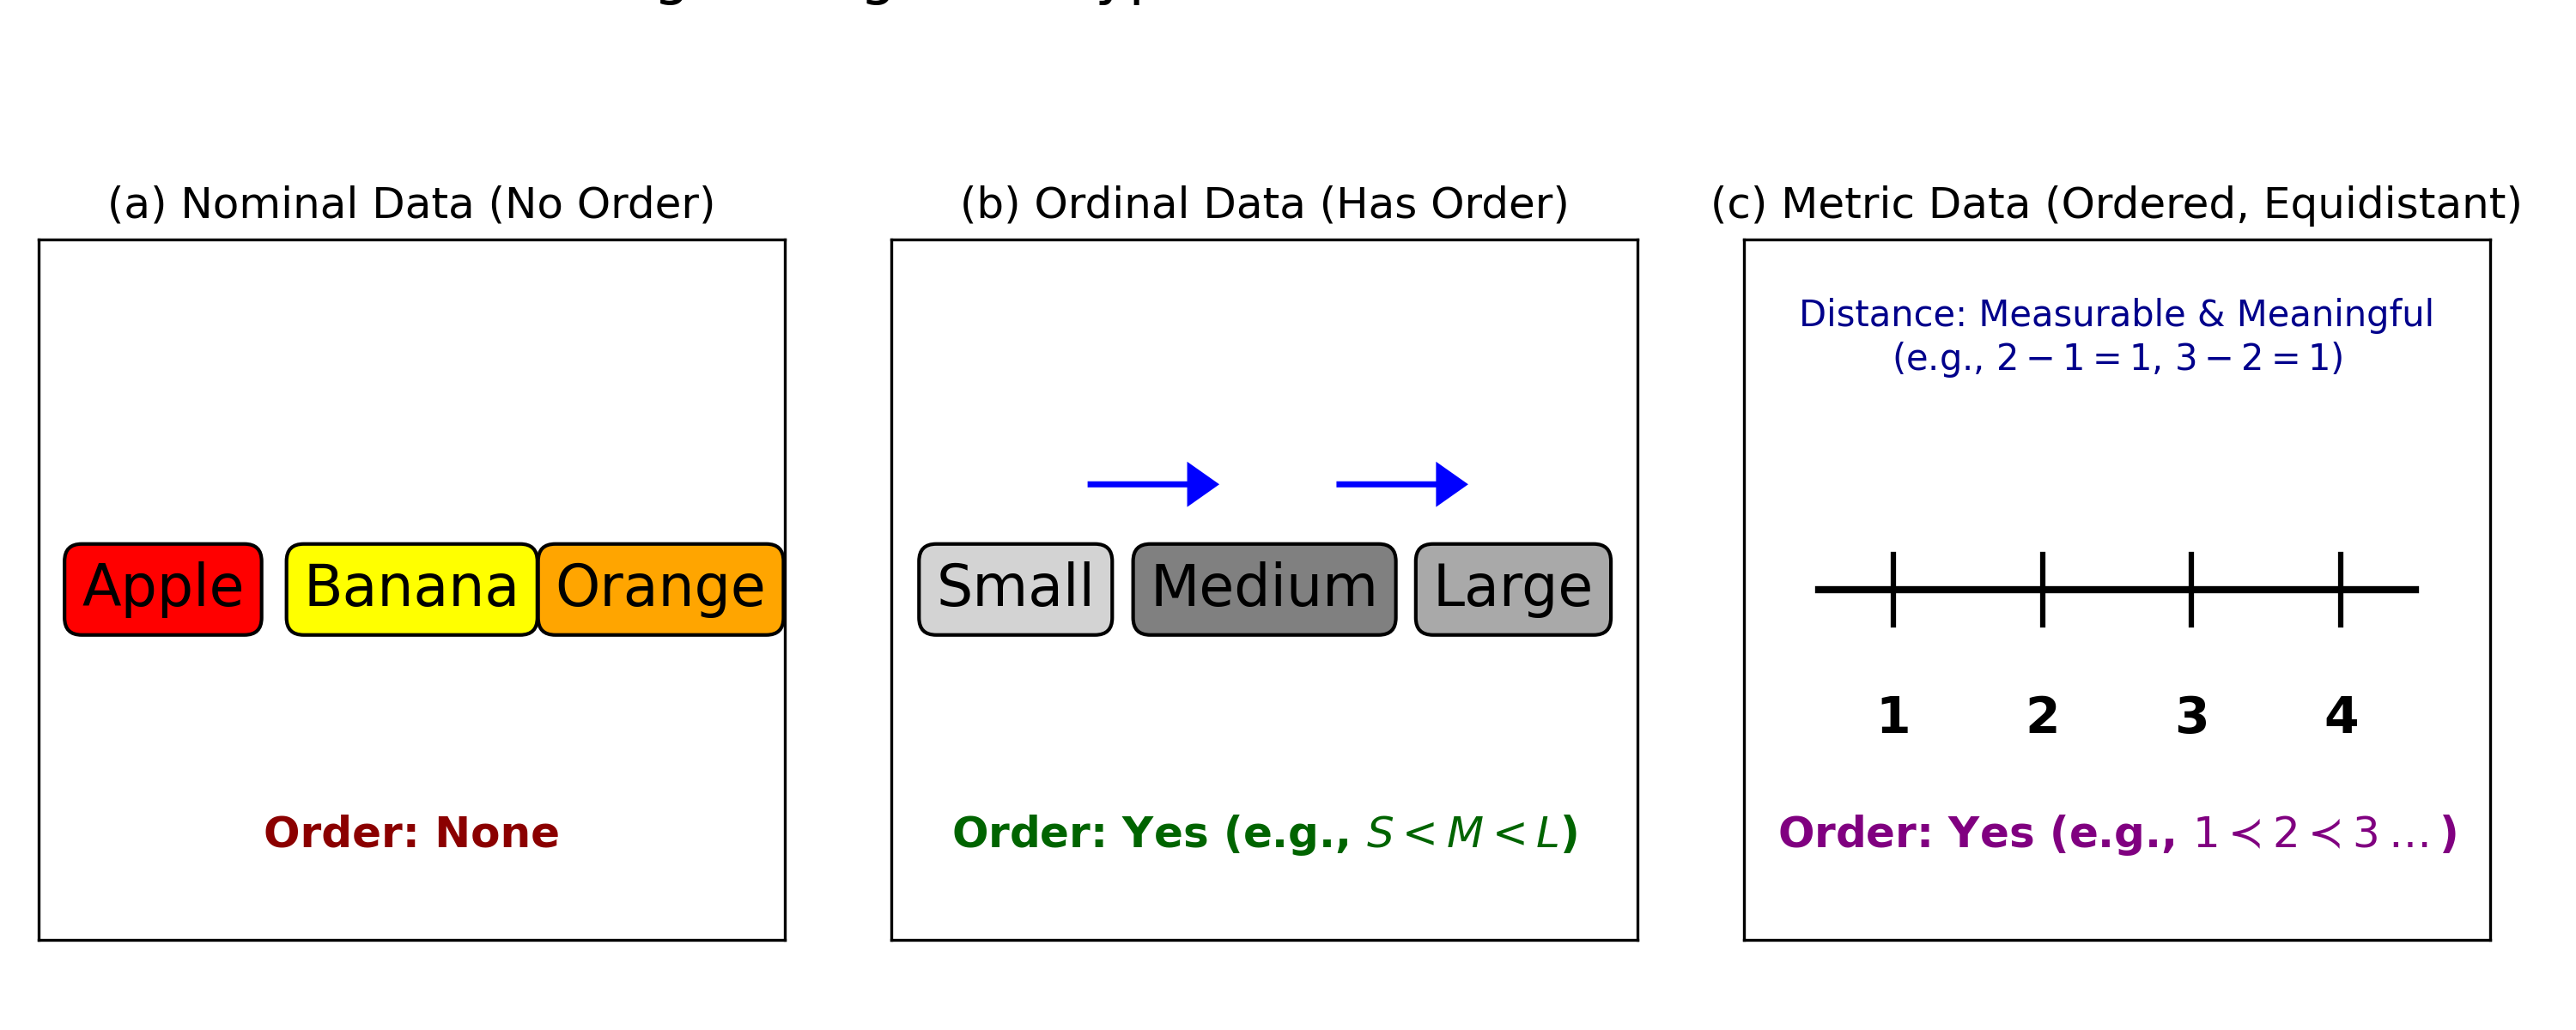
\includegraphics[width=0.9\textwidth]{assets/data_type_contrast.png}
  \caption{A conceptual comparison of data measurement scales, illustrating the unique nature of (b) Ordinal Data, where categories have a meaningful order but non-uniform distances, as seen in the oil contamination task.}
  \label{fig:data_types}
\end{figure}

To properly explore the performance of the transformer method for this challenging task, we compare our standard classification approach with three ordinal classification approaches. We use stratified k-fold cross-validation, Balanced Classification Accuracy (BCA), and Mean Average Error (MAE) to evaluate the accuracy. We use MAE to measure accuracy for ordinal classification because it effectively penalizes misclassifications based on their distance from the true category, a critical distinction from standard accuracy shown in Figure \ref{fig:eval_metrics}. The ordinal classification approaches we explore are:

\begin{figure}[htbp]
  \centering
  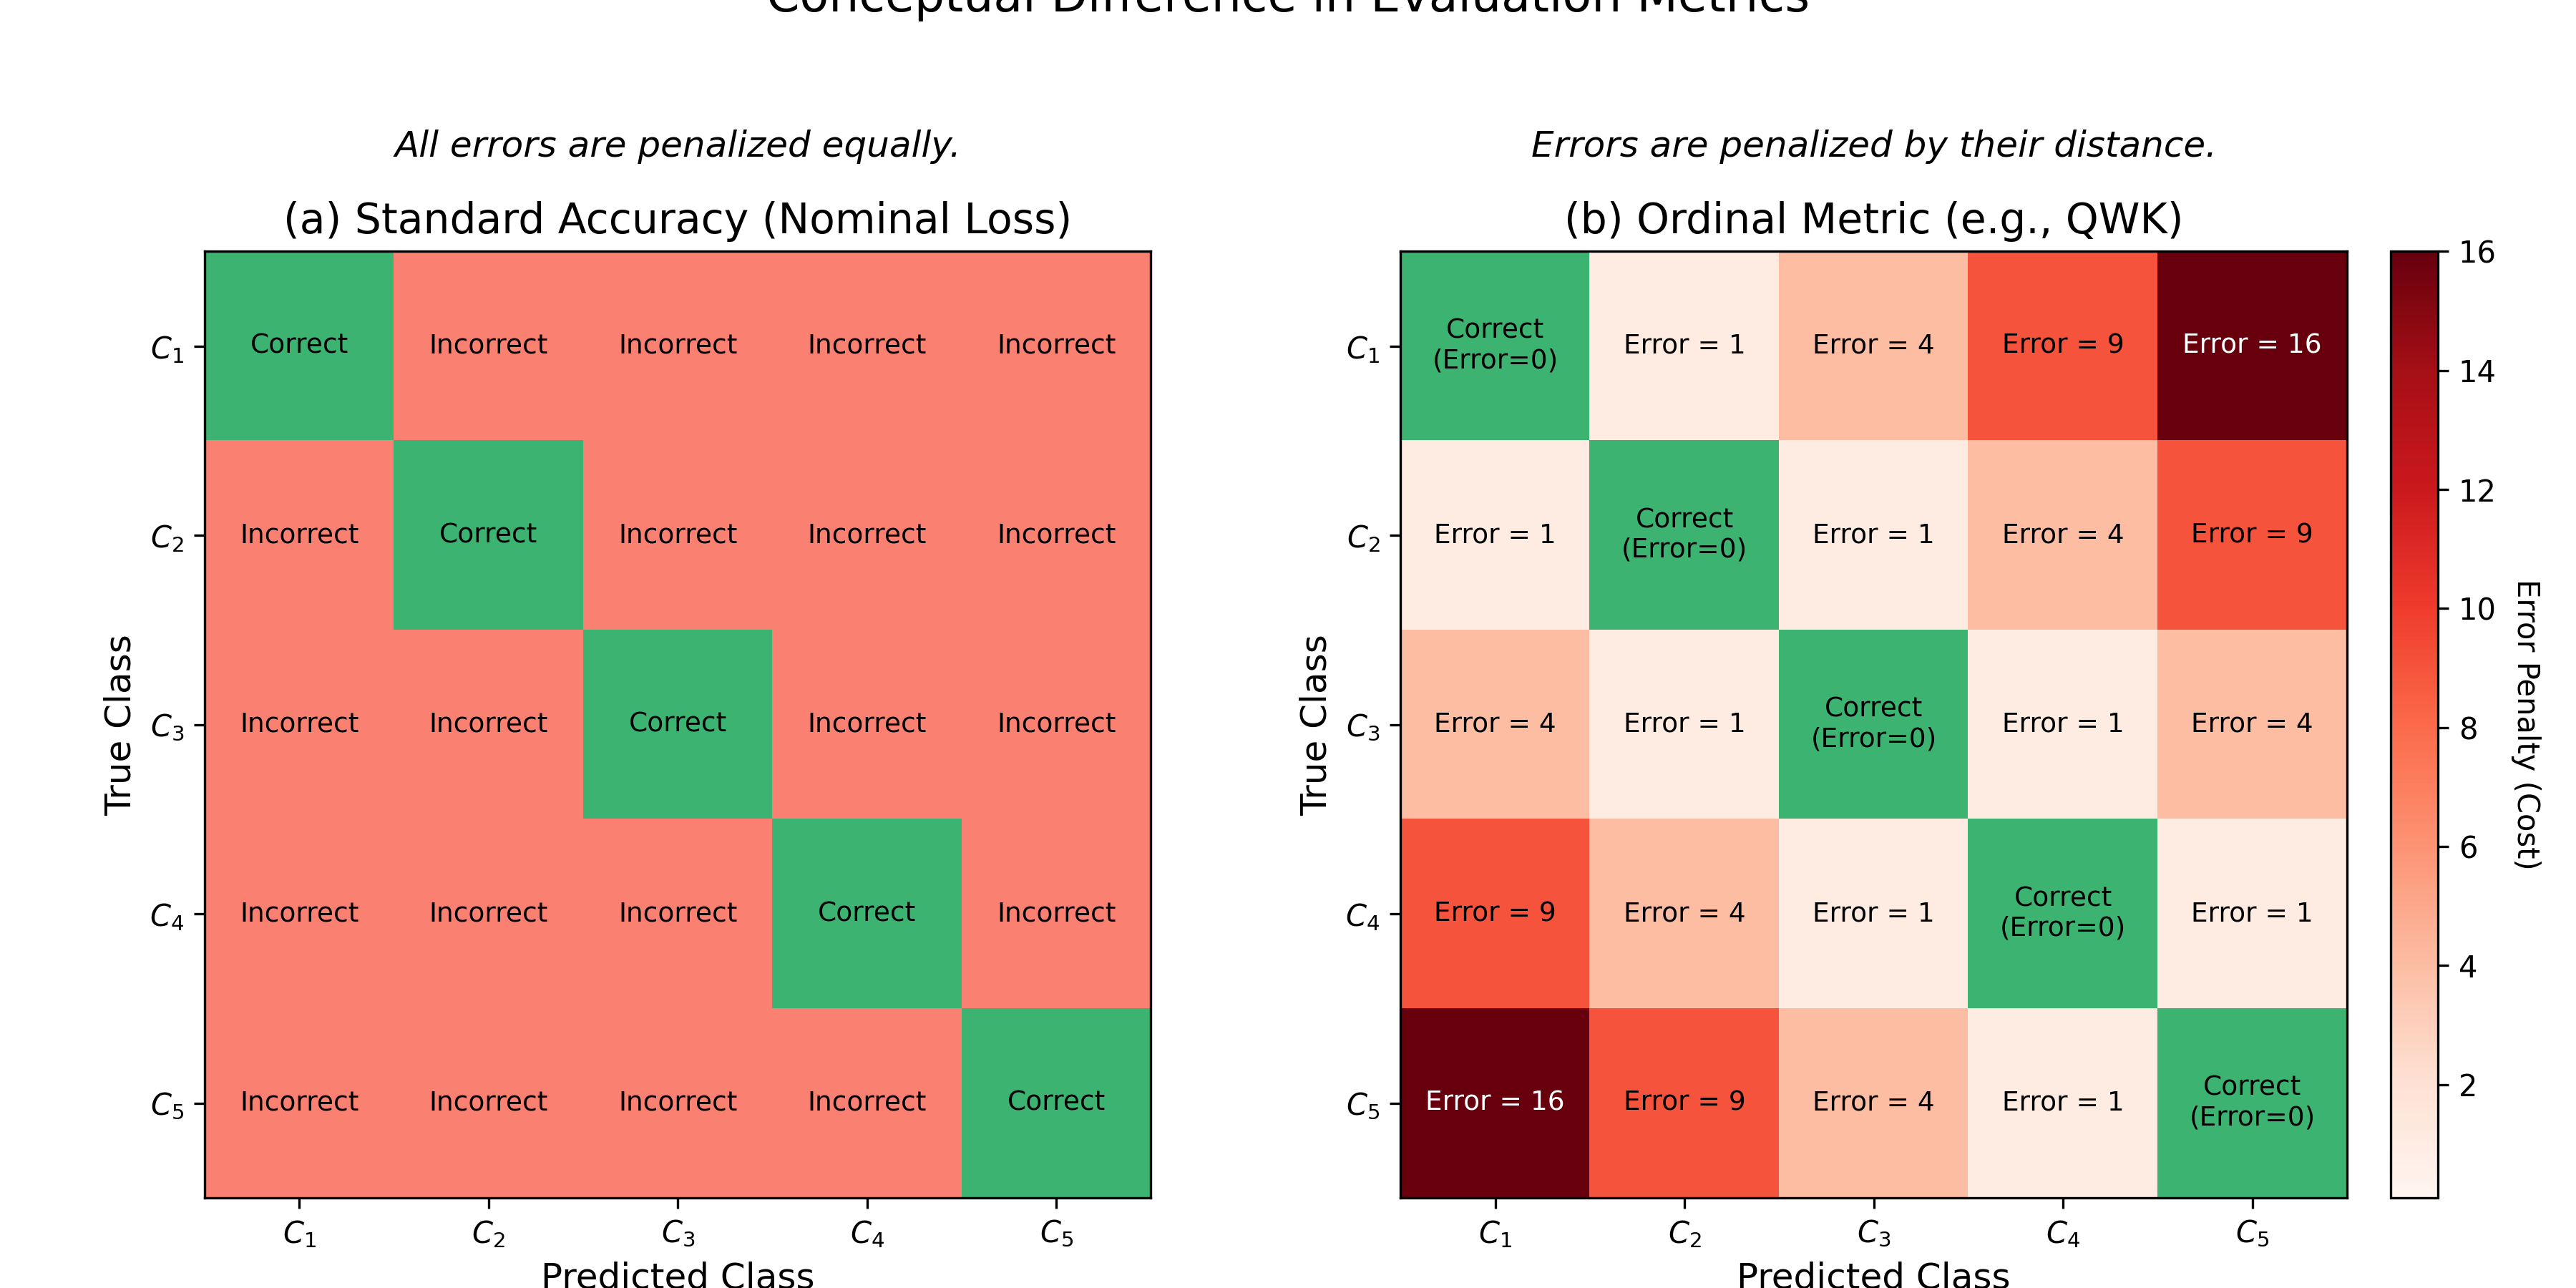
\includegraphics[width=0.9\textwidth]{assets/evaluation_metrics_contrast.png}
  \caption{Conceptual difference in evaluation. (a) Standard accuracy treats all misclassifications as equally incorrect (a 0-1 loss). (b) Ordinal metrics penalize errors based on their distance. This diagram illustrates a quadratic penalty, as used in Quadratic Weighted Kappa (QWK), which correctly identifies that a small error (e.g., predicting $C_4$ for $C_5$) is preferable to a large one (e.g., predicting $C_1$ for $C_5$).}
  \label{fig:eval_metrics}
\end{figure}

\begin{itemize}
    \item \textbf{Regression} \citep{Frank2001}: This approach treats the $K$ ordinal categories as continuous numerical values (e.g., $1, 2, 3, \cdots, K$). A standard regression model is trained to predict this value using a loss function like Mean Squared Error (MSE). The final predicted class is then obtained by rounding the continuous output to the nearest integer. This method is simple but assumes that the intervals between consecutive classes are equidistant.
    
    \item \textbf{Standard Classification}: This is the standard nominal approach, which treats the $K$ categories as independent, unordered labels. The model outputs a logit vector of size $K$ and is trained using a Cross-Entropy Loss. This method is fundamentally ``ordinal-blind," as it penalizes all misclassifications equally, regardless of their distance from the true label.

    The final two methods, CORAL and CLM, are modern deep learning strategies that explicitly model this ordinal structure, as conceptualized in Figure \ref{fig:dl_ordinal_strategies}.
    
    \item \textbf{CORAL} \citep{Cao2020}: The COnsistent RAnk Logits (CORAL) framework reframes the task using $K-1$ binary classifiers. Each classifier $i$ predicts the probability that the true label is greater than rank $i$ (i.e., $P(y > i)$). This is achieved using a shared set of weights and $K-1$ logits, trained with a binary cross-entropy loss. This design explicitly enforces the ordinal constraint, as predicting $y > i$ implies $y > i-1$. The final class is predicted by summing the number of logits that are positive (or have a probability $> 0.5$) and adding one.
    
    \item \textbf{Cumulative Loss (CLM)} \citep{Niu2016}: This method, based on cumulative link models, also learns $K-1$ outputs. These outputs represent the cumulative probabilities $P(y \le i)$. The model is trained to predict these cumulative probabilities, typically by learning a set of ordered thresholds (cutpoints) that partition the output of a shared feature extractor. The probability for a specific class $i$ is then derived from the difference between adjacent cumulative probabilities, $P(y=i)=P(y \le i)-P(y \le i-1)$, directly modeling the ordinal nature of the labels.
\end{itemize}

\begin{figure}[htbp]
  \centering
  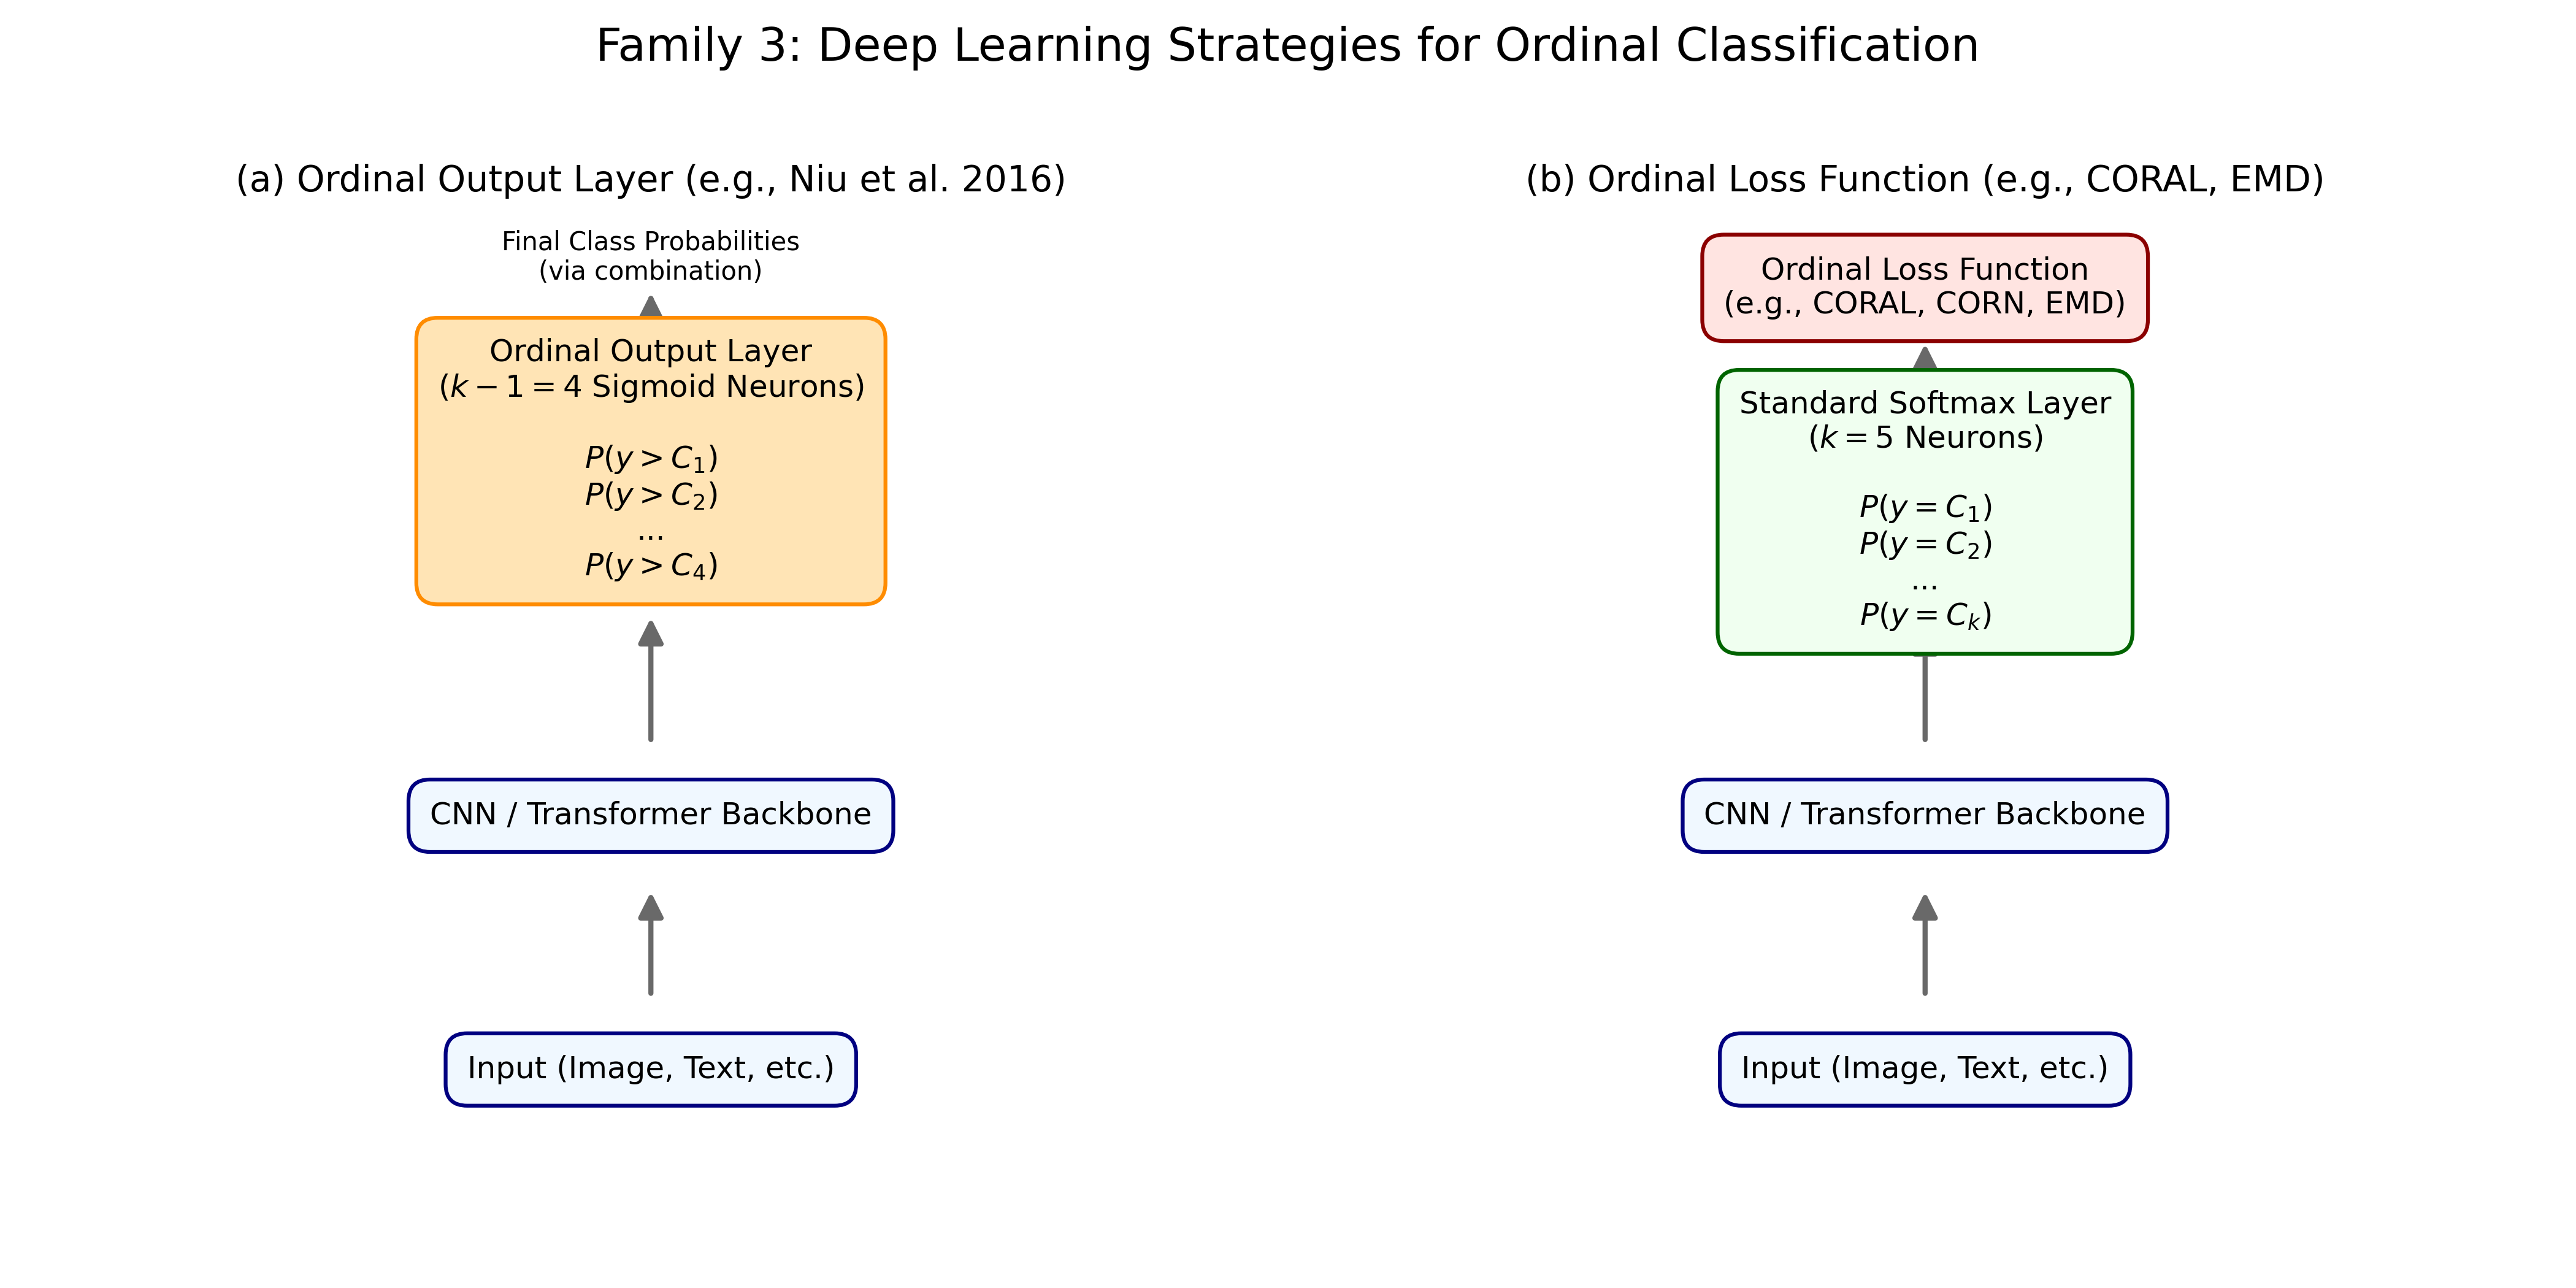
\includegraphics[width=\textwidth]{assets/deep_learning_ordinal_models.png}
  \caption{Common deep learning strategies for ordinal classification, showing the two approaches tested: (a) The Ordinal Output Layer approach, similar to CLM, which models cumulative probabilities, and (b) The Ordinal Loss Function approach, such as CORAL, which uses a specialized loss on a standard softmax output.}
  \label{fig:dl_ordinal_strategies}
\end{figure}

\begin{table}[htbp]
\centering
\caption{Final Cross-Validation Results}
\label{tab:cv_results}
\begin{tabular}{l cc cc}
\toprule
& \multicolumn{2}{c}{\textbf{TRAIN}} & \multicolumn{2}{c}{\textbf{TEST}} \\
\cmidrule(lr){2-3} \cmidrule(lr){4-5}
\textbf{Method} & \textbf{BCA} & \textbf{MAE} & \textbf{BCA} & \textbf{MAE} \\
\midrule
CLASSIFICATION  & 1.0000 $\pm$ 0.0000 & 0.0000 $\pm$ 0.0000 & 0.4519 $\pm$ 0.0573 & 1.7305 $\pm$ 0.2784 \\
REGRESSION      & 0.3436 $\pm$ 0.1726 & 1.0024 $\pm$ 0.4716 & 0.1476 $\pm$ 0.0551 & 1.6332 $\pm$ 0.1219 \\
CORAL           & 0.4856 $\pm$ 0.1725 & 0.8621 $\pm$ 0.3655 & 0.3048 $\pm$ 0.1023 & 1.5732 $\pm$ 0.1935 \\
CLM             & 0.5391 $\pm$ 0.1627 & 0.6856 $\pm$ 0.2618 & 0.2833 $\pm$ 0.1236 & 1.6145 $\pm$ 0.2957 \\
\bottomrule
\end{tabular}
\end{table}

The results table reveals a clear performance hierarchy among the different modeling approaches, strongly influenced by how each method handles the ordinal nature of the data. The standard classification approach achieves the highest training accuracy (1.0000 Mean BCA), but this comes at the cost of poor generalization, as evidenced by its mediocre test BCA (0.4519) and the highest test MAE (1.7305). This large gap between training and test performance indicates significant overfitting. Because this method is ``ordinal-blind," as illustrated in Figure \ref{fig:eval_metrics}(a), it treats the contamination levels as independent, unordered labels. While it can learn to perfectly separate these discrete categories in the training set, it fails to understand the inherent sequence (e.g., that 10\% contamination is closer to 5\% than to 50\%). Consequently, it penalizes all misclassifications equally, leading to a high average error distance on the test set.

In contrast, the regression-based approach demonstrates the poorest performance overall, with the lowest BCA on both the training (0.3436) and test (0.1476) sets. This underperformance can be attributed to its fundamental assumption that the ordinal categories can be treated as equidistant numerical values (e.g., 1, 2, 3...), as shown in Figure \ref{fig:data_types}(c). The low accuracy suggests this assumption is invalid for the oil contamination data; the perceived ``distance" between a 0\% and 1\% contamination level is likely not the same as between a 25\% and 50\% level. By converting the classification problem into a regression task and simply rounding the output, the model loses critical information about the class boundaries and struggles to make accurate discrete predictions.

The methods explicitly designed to handle ordinal data, CORAL and CLM, yield the most promising results for real-world applications. CORAL, in particular, strikes the best balance, delivering a competitive test BCA (0.3048) while achieving the lowest test MAE (1.5732). This superior MAE is a direct result of its architecture (see Figure \ref{fig:dl_ordinal_strategies}(b)), which uses a series of binary classifiers to enforce the rank ordering of the classes. The CLM method, which models cumulative probabilities (Figure \ref{fig:dl_ordinal_strategies}(a)), also performs well, producing a test MAE (1.6145) far better than the ordinal-blind methods. Together, these results underscore the importance of selecting a model that aligns with the data's underlying structure. For an ordinal task like grading contamination, models that incorporate this sequential information generalize more effectively and produce more meaningful predictions by minimizing the distance of errors. This trade-off between different model families is summarized in Table \ref{tab:strengths_weaknesses}, which compares the general strengths and weaknesses of each approach.

\begin{table*}[t]
\centering
\caption{Comparative Analysis of Ordinal Classification Model Families}
\label{tab:strengths_weaknesses}
\resizebox{\textwidth}{!}{%
\begin{tabular}{l l l l}
\toprule
\textbf{Family} & \textbf{Core Models} & \textbf{Strengths} & \textbf{Weaknesses} \\
\midrule
\textbf{1. Threshold-Based} & 
  POM, CLMs, SVOR & 
  \begin{tabular}[t]{@{}l@{}}
    - Statistically rigorous (POM/CLM) \\
    - Highly interpretable coefficients \\
    - Guarantees ordered predictions \\
    - Excellent on low-dim, tabular data
  \end{tabular} &
  \begin{tabular}[t]{@{}l@{}}
    - \textbf{Parallel Lines Assumption} is rigid \\
    - Can be hard to test/validate assumption \\
    - Less competitive on high-dim data \\
    - SVOR can be slow to train
  \end{tabular} \\
\midrule
\textbf{2. Binary Decomposition} & 
  Cumulative, Adjacent &
  \begin{tabular}[t]{@{}l@{}}
    - Conceptually simple and flexible \\
    - Can use \textit{any} binary classifier \\
    - No parallel lines assumption \\
    - Often highly competitive
  \end{tabular} &
  \begin{tabular}[t]{@{}l@{}}
    - Can lead to \textbf{inconsistent} probabilities \\
    - (e.g., $P(y>2)$ might be < $P(y>3)$) \\
    - Trains $k-1$ models, which can be slow \\
    - Less direct interpretation
  \end{tabular} \\
\midrule
\textbf{3. Deep Learning} & 
  CORAL, CORN, EMD Loss &
  \begin{tabular}[t]{@{}l@{}}
    - State-of-the-art on high-dim data \\
    - (Images, text, etc.) \\
    - No strong statistical assumptions \\
    - Can be built into any NN architecture
  \end{tabular} &
  \begin{tabular}[t]{@{}l@{}}
    - Requires large datasets \\
    - Prone to overfitting on small data \\
    - ``Black box" / less interpretable \\
    - Computationally expensive
  \end{tabular} \\
\bottomrule
\end{tabular}%
}
\end{table*}

\section{Chapter Summary}
\label{sec:conclusion-and-future-work}

Our research demonstrates that deep learning models can revolutionize REIMS-based marine biomass analysis.

\subsection{Conclusions}

This chapter concludes that the novel unsupervised pretraining method, ``Masked Spectra Modeling" (MSM), shows task-dependent effectiveness. MSM proves valuable for difficult problems like oil contamination detection—a challenging ordinal classification task—where it successfully improves the model's performance. This is likely because the pretraining task, which implicitly learns to predict spectral peaks, mirrors the techniques chemists use to analyze REIMS data and provides a strong foundation for identifying subtle chemical signals. However, for tasks with more distinct signatures like cross-species adulteration, pretraining was detrimental to performance.
In terms of architecture, the Mixture of Experts (MoE) Transformer outperforms the regular Transformer on the majority of the classification tasks, as its divide-and-conquer strategy of using specialized expert networks improves the balanced accuracy score. Furthermore, transfer learning with the MoE Transformer consistently benefits the difficult oil contamination task regardless of the source task, indicating that for this specific challenge, the performance increase justifies the additional computation required.
Finally, our analysis of the methods applied to the oil contamination task revealed that the distance-aware loss functions we tested, even those from a simple regression approach, dramatically outperformed the standard `ordinal-blind' classification. Furthermore, the more complex, specialized ordinal models we evaluated offered additional, though more modest, performance benefits for this specific task.

\subsection{Future Work}

While our study has yielded promising results, several important areas warrant further investigation:

\begin{enumerate}
    \item \textbf{Overfitting for Oil Contamination:} Address the significant overfitting issue for oil contamination with further exploration of ordinal classification techniques.
    \item \textbf{Multi-modal Data Fusion:} Combine REIMS data with other analytical techniques (e.g., Near-infrared spectroscopy or DNA barcoding) to create more robust classification systems that leverage complementary information sources. This could improve accuracy in challenging cases where single-modality analysis is insufficient.
    \item \textbf{Transfer Learning Across Species:} Investigate whether models trained on Hoki and Mackerel can transfer their learned features to detect contamination in other fish species, potentially reducing the need for extensive new training data.
    \item \textbf{Causes of Asymmetric Transfer:} The underlying causes of the asymmetric transfer effects, particularly why oil classification consistently benefits from transfer, while other domains do not.
    \item \textbf{Transfer Learning Feature Embeddings:} Additionally, exploring the feature representations learned in each domain could provide valuable insights into why certain transfers are more successful than others.
\end{enumerate}